
%\documentclass[12pt,oneside,reqno]{amsart}
%\documentclass[12pt,oneside]{amsart}
%\usepackage{amssymb}
\documentclass[parskip=full,12pt,a4paper]{report}
\usepackage{fontspec}
%\setmainfont[Mapping=text-tex]{OpenSans}
\setsansfont{OpenSans}[
    Path=./strfont/,
    Scale=0.9,
    Extension = .ttf,
    UprightFont=*-Regular,
    BoldFont=*-Bold,
    ItalicFont=*-Italic,
    BoldItalicFont=*-BoldItalic
    ]


%\setmainfont{OpenSans}[ 
%Extension = .ttf,
%UprightFont = *-Regular]
\setmainfont[Ligatures=TeX,
    Path=./strfont/,
    Scale=0.9,
    Extension = .ttf,
    UprightFont=*-Regular,
    BoldFont=*-Bold,
    ItalicFont=*-Italic,
    BoldItalicFont=*-BoldItalic
    ]{OpenSans}

\setsansfont{OpenSans}[
    Path=./strfont/,
    Scale=0.9,
    Extension = .ttf,
    UprightFont=*-Regular,
    BoldFont=*-Bold,
    ItalicFont=*-Italic,
    BoldItalicFont=*-BoldItalic
    ]

\setromanfont{OpenSans}[
    Path=./strfont/,
    Scale=0.9,
    Extension = .ttf,
    UprightFont=*-Regular,
    BoldFont=*-Bold,
    ItalicFont=*-Italic,
    BoldItalicFont=*-BoldItalic
    ]
    
\setmonofont{OpenSans}[
    Path=./strfont/,
    Scale=0.9,
    Extension = .ttf,
    UprightFont=*-Regular,
    BoldFont=*-Bold,
    ItalicFont=*-Italic,
    BoldItalicFont=*-BoldItalic
    ]
    
\usepackage{hyperref}
\hypersetup{
    colorlinks=true,
    linkcolor=blue,
    filecolor=magenta,      
    urlcolor=cyan,
    pdftitle={MSc Dissertation},
    pdfpagemode=FullScreen,
    }



%\setmainfont[Ligatures=TeX]{Calibri.ttf}

%\setmainfont[Ligatures=TeX]{str_uni_font/Calibri.tff}
%\setmainfont{[CrimsonText-str_uni_font/calibri.tff]}
\usepackage[export]{adjustbox}

\usepackage[left=2.8cm, right=2.8cm]{geometry}
% with 12 point font, single line spacing, single-sided pages
\setlength{\textheight}{23cm}
\setlength{\footskip}{1.5cm}
\usepackage[singlespacing]{setspace} % don't use onehalfspacing
\usepackage{titlesec}
\usepackage{parskip}
\setlength{\parindent}{0em}
\setlength{\parskip}{1em}

\usepackage{IEEEtrantools}
\usepackage{ctable}
\usepackage{array}
\usepackage{comment}
\usepackage[dvipsnames]{xcolor}
\newcolumntype{?}{!{\vrule width .618pt}}
%\usepackage[margin=2.5cm]{geometry}

\usepackage{mathptmx}


\usepackage{listings} % for source code
\definecolor{codegreen}{rgb}{0,0.6,0}
\definecolor{codegray}{rgb}{0.5,0.5,0.5}
\definecolor{codepurple}{rgb}{0.58,0,0.82}
\definecolor{backcolour}{rgb}{0.95,0.95,0.92}

\lstdefinestyle{mystyle}{
    backgroundcolor=\color{backcolour},   
    commentstyle=\color{codegreen},
    keywordstyle=\color{magenta},
    numberstyle=\tiny\color{codegray},
    stringstyle=\color{codepurple},
    basicstyle=\sffamily\footnotesize,
    breakatwhitespace=false,         
    breaklines=true,                 
    captionpos=b,                    
    keepspaces=true,                 
    numbers=left,                    
    numbersep=5pt,                  
    showspaces=false,                
    showstringspaces=false,
    showtabs=false,                  
    tabsize=2
}

\lstset{style=mystyle}


\usepackage[style=ieee,
defernumbers=false, 
backend=biber, 
maxnames=1 ,
sortcites=true,
maxcitenames=1,
maxbibnames=6,
giveninits=true, 
uniquename=false,
uniquelist=false, 
url=true,
doi=true,
issn=false,
isbn=false]{biblatex}
%\usepackage[style=ieee,uniquelist=false,giveninits=true,,maxbibnames=9,maxcitenames=2,backend=biber]{biblatex}

\addbibresource{References.bib}
\addbibresource{sentinel.bib}

%% pretty captions
\usepackage{caption}
\usepackage{subcaption}
\usepackage{wrapfig}
%set fontsize for figure captions
\captionsetup[figure]{font=tiny}
\usepackage[font=normalsize,labelfont={bf}]{caption}
%%% takes copy of jpg/png while drafting
\setlength{\fboxsep}{0.005pt}
 \newcommand{\tmpframe}[1]{\fbox{#1}}
 \captionsetup[figure]{skip=6pt}
%%% allows you to create Rules, Definitions, Lemmas, Theorems etc.
\usepackage{amsthm}
\usepackage{amsmath}
\usepackage{amsfonts}
\usepackage[]{algorithm2e}
% --------------------- here!!! ------------------------

\newtheorem{theorem}{Theorem}
\newtheorem{definition}{Definition}
\newtheorem{lemma}{Lemma}
\newtheorem{Rule}{Rule}
\numberwithin{definition}{chapter}
\numberwithin{theorem}{chapter}  
\numberwithin{lemma}{chapter}  
\numberwithin{Rule}{chapter}  
\numberwithin{equation}{chapter} 
\newcommand\tab[1][1cm]{\hspace*{#1}}

\usepackage[super]{nth} 
 
\usepackage{graphicx}
\usepackage{wrapfig}
\usepackage{placeins}
\usepackage{pdfpages}
\usepackage{attachfile2}
\usepackage{float}

%\usepackage[utf8]{inputenc}
%\usepackage[T1]{fontenc}
\usepackage{csquotes}
\usepackage{ragged2e}
\usepackage{blindtext}
\usepackage{fancyhdr}
\usepackage{epigraph}
%\pagestyle{fancy}
\renewcommand{\headrulewidth}{0.4pt}
%\renewcommand{\footrulewidth}{0.4pt}
\fancyhead{}
\fancyhead[L]{ATTENTION to IAQA} %%% CHANGE AS APPROPRIATE (you may need to use a shortened form of the title)
\fancyhead[R]{Student ID: 2935530} 
\fancyfoot{}
\fancyfoot[C]{\thepage}

\usepackage{titlesec}

%% prevents Chapter 1 (then new line and Introduction) - turns into 1. Introduction


% Call your references "References" rather than Bibliography, then also allow for a separate Bibliography if needed.

\DeclareSourcemap{
  \maps[datatype=bibtex]{
    \map{
      \perdatasource{References.bib}
      \step[fieldset=keywords, fieldvalue={, primary}, append]
    }
    \map{
      \perdatasource{bibleo.bib}
      \step[fieldset=keywords, fieldvalue={, secondary}, append]
    }
  }
}
%%%%%%%%%%%%%%%%%%%%%%%%%%%%%%%%
%  Don't make any changes here
%  This defines formatting style
%%%%%%%%%%%%%%%%%%%%%%%%%%%%%%%%

\DeclareNameAlias{sortname}{last-first}
\DeclareFieldFormat{edition}{%
  \ifinteger{#1}
    {\ifnumequal{#1}{1}%
     {}%
     {\mkbibordedition{#1}~\bibstring{edition}}%
    }
    {#1\isdot}}

\DeclareFieldFormat[article,inbook,incollection]{title}{#1\isdot}
\DeclareFieldFormat[article,inbook,incollection]{citetitle}{#1\isdot}

\newrobustcmd{\MakeTitleCase}[1]{%
  \ifboolexpr{test {\ifentrytype{article}} or test {\ifentrytype{inbook}} or test {\ifentrytype{incollection}}}
    {#1}
    {\MakeSentenceCase{#1}}}

\DeclareFieldFormat{urldate}{\bibsentence\mkbibbrackets{\bibstring{urlseen}\space#1}}
\DeclareFieldFormat{url}{\bibstring{urlfrom}\addcolon\space\url{#1}}

\renewbibmacro*{journal}{%
  \iffieldundef{journaltitle}
    {}
    {\printtext[journaltitle]{%
       \printfield[titlecase]{journaltitle}%
       \setunit{\subtitlepunct}%
       \printfield[titlecase]{journalsubtitle}}
       \ifboolexpr{
         not test {\iffieldundef{url}}
         or
         not test {\iffieldundef{urldate}}
         or
         not test {\iffieldundef{doi}}
         or
         not test {\iffieldundef{eprint}}
       }
         {\nopunct\bibstring[\mkbibbrackets]{online}}%
         {}}}

\renewbibmacro*{journal+issuetitle}{%
  \usebibmacro{journal}%
  \setunit*{\addspace}%
  \iffieldundef{series}
    {}
    {\newunit
     \printfield{series}%
     \setunit{\addspace}}%
  \newunit
  \usebibmacro{volume+number+eid}%
  \setunit{\addspace}%
  \usebibmacro{issue+date}%
  \setunit{\addcolon\space}%
  \usebibmacro{issue}%
  \newunit}

\NewBibliographyString{online}
\DefineBibliographyStrings{english}{%
  urlseen    = {accessed},
  online     = {online},
}
%\addbibresource{example.bib}
\renewcommand*{\nameyeardelim}{\addcomma\addspace}
\renewbibmacro{in:}{%
  \ifentrytype{article}{}{\printtext{\bibstring{in}\intitlepunct}}} % removes "In" preceeding journal title
  
  
\setcounter{tocdepth}{3} % allow only sections (not subsections in table of contents)


\setlength{\textheight}{23cm}
%\setlength{\footskip}{1.5cm}

\titlespacing*{\chapter}{0pt}{-50pt}{20pt}
\titleformat{\chapter}[hang]{\normalfont\huge\bfseries}{\thechapter}{1em}{} 
\newcommand{\cmd}[1]{\texttt{\textbackslash{}#1}}
\newcommand{\unnumberedchapter}[1]{\chapter*{#1}\addcontentsline{toc}{chapter}{#1}}  
\let\tempit\itemize \let\tempeit\enditemize \renewenvironment{itemize}{\vspace{-1em}\tempit\addtolength{\itemsep}{-0.5\baselineskip}}{\tempeit} % Changes itemize spacing
\let\tempen\enumerate \let\tempeen\endenumerate \renewenvironment{enumerate}{\vspace{-1em}\tempen\addtolength{\itemsep}{-0.5\baselineskip}}{\tempeen} % Changes enumerate spacing
%%%%%%%%%%%%%%%%%%%%%%%%%%%

% with 12 point font, single line spacing, single-sided pages

\setlength{\textheight}{23cm}
%\setlength{\footskip}{1.5cm}



\begin{document}

\setmainfont[Ligatures=TeX,
    Path=./strfont/,
    Scale=0.9,
    Extension = .ttf,
    UprightFont=*-Regular,
    BoldFont=*-Bold,
    ItalicFont=*-Italic,
    BoldItalicFont=*-BoldItalic
    ]{OpenSans}





\pagenumbering{roman}
\begin{titlepage}
    
    % \raisebox{1cm}[0pt][0pt]{}
    \centering
    
\includegraphics[width=0.4\linewidth]{logos/primary-logo.jpg}
    \begin{center}
        \vspace*{1cm}
          \vspace{10mm}
        {\large Division of Computing and Mathematics\\
        \large Faculty of Natural Sciences \\
        \textsc{University of Stirling}}
        \\
        \vspace{0.5cm}
        {\large
        Paying Attention to Image Aesthetic Quality Assessment}
        \vspace{0.5cm}
        \\
        {\large By}
        \\
        \vspace{0.5cm}
        \textbf{de Sigley, Frida}\\
        \vspace{0.5cm}
        \textbf{Student Number: 2935530}
   		\vspace{1.5cm}
        \vspace{0.25cm}
       \\
        \vspace{0.25cm}
    

      

        \vspace{0.8cm}
        \begin{minipage}{10cm}
        \center Dissertation submitted in partial fulfillment for the the degree of \\
        \textsc{Master of Science in Artificial Intelligence}.
        \end{minipage}\\
        \vspace{0.8cm}
        \today
        
    \end{center}
    
 

\end{titlepage}
\chapter*{Declaration of own work}

I understand the nature of plagiarism, and I am aware of the University’s policy on this.
I certify that this dissertation reports original work by me during my University project except for the following:

\

\begin{itemize}
    \item Transformer code used in experiments chapter \ref{transformer_method} in was taken from Facebook (now Meta) AI GitHub\footnote{\href{https://github.com/facebookresearch/convit}{https://github.com/facebookresearch/convit}} and taken in modified form\footnote{\href{https://github.com/mawady/convit}{https://github.com/mawady/convit}}
    \item Pre-Trained models used in chapter \ref{chap:Methodology} courtesy of Ross Wightman\footnote{\href{https://github.com/rwightman/pytorch-image-models}{https://github.com/rwightman/pytorch-image-models}}  
    \item The training loop in was adapted from PyTorch example of training loop provide in a notebook 
    \item Formative model training of various transformers Was made using code from Phil Wang\footnote{\href{https://github.com/lucidrains/vit-pytorch}{https://github.com/lucidrains/vit-pytorch}}
    \item While all other code was written by the author, there are some sections where code has been adapted from other sources - such as loss function examples\footnote{\href{https://github.com/clcarwin }{https://github.com/clcarwin/focal\_loss\_pytorch }} 
    \item Unless explicitly cited, all figures are originally produced by the author. Where figures are taken from publications, citation(s) are included in the image caption; where images are taken from data-sets and then manipulated graphically, the associated data-set of the publication is used. For instance, figure \ref{fig:MNIST 5} is from MNIST\cite{LeCun1998}, but the image plot, patches, and graphical manipulation are original. 
    \item Reproducing results from \cite{Sheng2018a,Hosu2019,Talebi2018,Ma2017} was done using associated GitHub repositories\footnote{\href{https://github.com/Openning07/MPADA}{https://github.com/Openning07/MPADA}}
    \footnote{\href{https://github.com/subpic/ava-mlsp}{https://github.com/subpic/ava-mlsp}}
    \footnote{\href{https://github.com/idealo/image-quality-assessment}
    {https://github.com/idealo/image-quality-assessment}}
    \footnote{\href{https://github.com/GuillaumeBalezo/A-Lamp}{https://github.com/GuillaumeBalezo/A-Lamp}}
    \item The dissertation was proof read Laura Whyte for typographic errors and miss spellings. 

\end{itemize}
Frida de Sigley\\

\includegraphics[width=0.2\textwidth]{figures/signature/Signature.jpg}\\
\today

 \begin{flushright}
 
\end{flushright}

\newpage
\chapter*{Acknowledgements}
% Add here text if you would like to thank somebody, e.g., your family, friends, colleagues, supervisors, etc.

I would like to thank  Dr Mohamed Elsayed Elawady, Dr Deepayan Bhowmik, Dr Kevin Swingler for there ongoing patience with my incessant questioning; their sound academic guidance and their genuine moral support, because deep learning is a deep subject. I would also like to thank my partner Laura Whyte for ongoing support and proof reading and thank my parents Linda Nelson and Jeremy Penford for their support throughout. Finally I would like to thank the Marian Dunbar for being such and enthusiastic proponent of Scottish Data and Tech and  the DataLab Scotland whose funding made undertaking an MSc in Artificial Intelligence possible.  
    




\chapter*{Abstract}
This thesis examines Image Aesthetic Quality Assessment(IAQA) as a computer vision problem. We compare deep Convolutional Neural Networks (CNNs) with Vision Transformers (ViTs) and Convolutional Vision Transformers (ConViTs), and examine which models best predict 'image quality' as a binary classification problem. 

While CNNS have superseded hand-crafted approaches to feature extraction, achieving this has required hand-crafting attention mechanisms as high level training policies on very complex CNN architectures - which are, themselves, time consuming and inefficient to train. We therefore produce a side-by-side comparison to assess whether self-attention can perform well as an IAQA classifier.  

We perform training on the AVA Bench-marking dataset and show that in many cases both ViTs and ConVits outperform CNNs in side-by-side comparisons. Further, while ViTs and ConVits both require lengthy pre-training on very large datasets, they are excellent candidates for domain adaptation - often with pre-trained models performing well when architectural adjustments are made to output layers. 

Surprisingly, this requires fewer training epochs than pre-trained CNN models to adapt to new domains. Further, while CNNs quickly overfit on the AVA Training subset, this is not the case with transformers. We also show that the conditions that suit each type of network differ, however, ConVits do not appear to require as many 'warm-up' epochs when being trained using transfer learning as they do in when being initially trained. 

We show that while models will train on the AVA benchmarking dataset without pre-training, that using non pre-trained models does not achieve high training accuracy.  
%

Total Words:
15046
Headers:
83
Math Inline:
126
Math Display:
17
\vfill
\begin{flushright}
\begin{longtable}
    \centering
    \begin{tabular}{c|c}
    Total Words & 15046 \\
    Headers & 83 \\
    Inline Equations & 126\\
    Equations & 17\\
    \end{tabular}
    \caption{Caption}
    \label{tab:my_label}
\end{longtable}
\end{flushright}
    
 %% any other "Front matter" should go here before the table of contents - format in a style similar to the file Abstract.tex
%%\usepackage{amsmath}
 % not here ... look up!!
\tableofcontents 
\listoftables
\lstlistoflistings
\newpage
\listoffigures

\addtocontents{toc}{~\hfill\textbf{Page}\par} % comment this line out if you want to remove "Page"
\pagenumbering{arabic}
\setcounter{page}{0}
%%%%%%%%%%%%%%%%%%%%%%%%%%%%%%%%%%%%
\chapter{Introduction}
\label{chap:Introduction}
%%%%%%%%%%%%%%%%%%%%%%%%%%%%%%%%%%%%



\section{Background}
\label{background}
\epigraph{We are of course, supposing for the present that the questions are of the kind to which an answer `Yes' or `No' is appropriate, rather than questions such as `What do you think of Picasso?'\cite{TURING1950}}{\textit{Alan M. Turing
}}

Image aesthetic assessment as a computational and machine learning task is important, challenging and fascinating. The application of aesthetics is wide, and encompasses areas such as cosmetics, calligraphy, and painting alongside beauty prediction of digital portraits\cite{Redi2015a} and facial beauty prediction\cite{Gray2010,Eisenthal2006a, Zhang2016}. Applications within the art domain include style recognition\cite{Cho2020, Fernando2021} and aesthetic visual quality of handwriting\cite{Sun2015}. All of these approaches require some form of digital imagery, and this thesis will focus on the Aesthetic Quality Assessment of digital images in the form of digital photographs. \par 

Within computer vision, there are sub-domains where aesthetics is a component such as Image Quality Assessment(IQA)\cite{Gu2020,Seshadrinathan2009,Sheikh2005,Ke2006,Chubarau2021,Reisenhofer2018} and Image Restoration, which have used metrics such as PSNR and SSIM. However, Image Aesthetic Quality Assessment(IAQA) treats aesthetic prediction as a target rather than focusing necessarily on individual image properties. Where IQA and image restoration have focused on restoring objective image distortions and are aimed at modelling or predicting a physical property such that it can be removed, IAQA focuses on predicting classes or aesthetics attributes.

\par
 
While aesthetic is often based on individual subjective perception, it is important to demarcate this from objective and empirical study within the field of machine learning and pattern recognition. Where the focus is on objective ground truth, whether by experts or aggregated scores, the computer vision task is to best predict ground truth. The perceptual element, alongside the potential for ambiguity and lack of consensus on concepts such 'beauty' and 'aesthetic appreciation'\cite{Datta2006}, add to the complexity and the challenge of IAQA\cite{Yang2019} as a machine learning problem. One aspect of this is that it includes human visual perception, which has been shown within psychological studies to be both contingent upon the target photograph's context\cite{Mullennix2020}, where the order in which images are viewed effects aesthetic perception, and to differ significantly between subjects\cite{Younes2016}. 

\newpage

IAQA's reliance upon high-level social concepts\cite{Datta2006} is however part of what makes the field so fascinating; with the potential to further insights into human visual attention, perception, and cognition\footnote{\textit{Vision} it might be argued it is a form of perception, property of cognition and intelligence\cite{russell2016artificial} . Pigeons for instance have been shown to be remarkable observers of pathology \cite{Levenson2015} when rewarded appropriately.
} and continue a valuable tradition of biologically inspired computing\cite{Hassabis2017} that began in the 1950s, in addition of course to IAQA's significant commercial and practical applications. 

\par 
Computer vision has made significant gains in tasks such as object recognition, classification, medical imaging\cite{Esteva2021}.  The problem of 'vision' is however far from solved; for example, semantic scene detection remains a challenging area of focus. This is complex in part because it requires consideration of whether image segmentation \textit{or} recognition comes first\cite{Kreiman2021} (a task that can also be a challenge for humans) (see figure \ref{fig:vase_face}). IAQA is one such challenging domain application.\par



\begin{figure}[h!]
    \centering
    \subfloat[Vase Face Figure Ground ambiguity f \cite{Hobbs1990,Eysenk2012}]{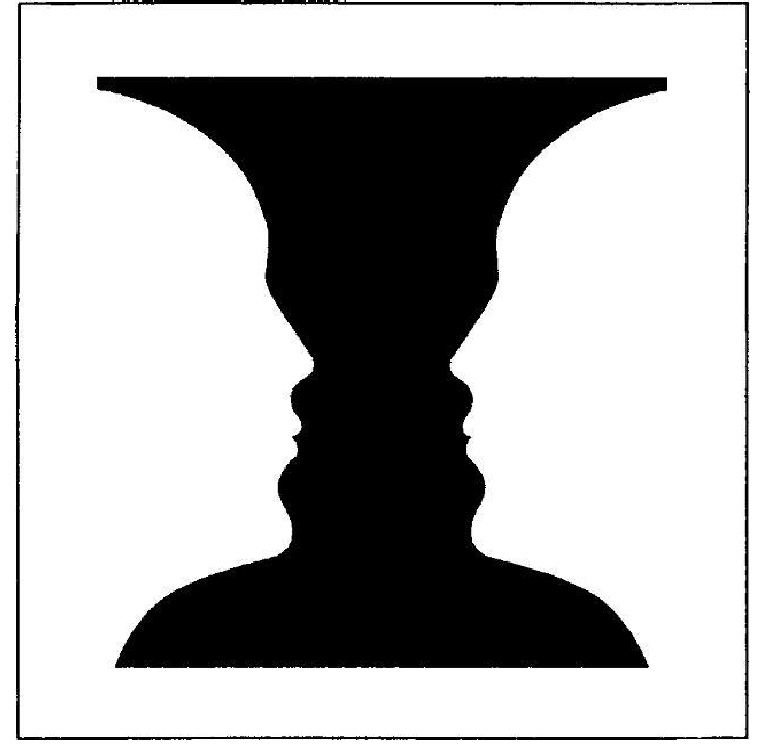
\includegraphics[height=0.2\textwidth]{figures/introduction/face-vase-face.png}}
    \subfloat[ An average face with a Phi mask not fitting the average face well \cite{Zhang2016}]{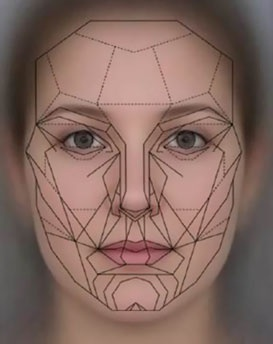
\includegraphics[height=0.2\textwidth]{figures/introduction/1492016_Book_ComputerModelsForFacialBeautyA.pdf1.jpeg}}
    \caption{Examples of Ambiguity for Machines and Humans}
    \label{fig:vase_face}
\end{figure}

\par

Traditional approaches to IQA have aimed at measuring image distortion by degrees\cite{gonzalez2008digital} within the wider field of digital image restoration. IQA's focus on modelling the non-commutative and non associative process of restoring digital image distortions caused by the corpuscular nature of light such as diffraction, refraction or image sensor noise caused during the capture of digital images in low light conditions.\cite{szeliski2011computer,gonzalez2008digital} have informed approaches to early approaches IAQA. In both IAQA and IQA, traditional computer vision has been superseded by Machine Learning(ML) in many areas, using techniques such as Deep Learning using convolutional neural networks (CNNs) which have been successfully employed since first used for character recognition\cite{LeCun1989,LeCun1998}.  \par
This thesis will examine how these more recent techniques have been applied to challenging domain application of IAQA, and seek to improve and  demonstrate effectiveness of different deep learning approaches within IAQA.

\newpage


\subsection{The Application Domain}

The Oxford English Dictionary(OED) defined 'aesthetics' as 'Of or relating to the perception, appreciation, or criticism of that which is beautiful'\cite{OED2021}. Aesthetics more widely includes appreciation of all senses, including touch and olfactory sensation\cite{Hayes2015}, and further cognitive activities such as mathematical problem solving which have an element of reward or pleasure, where we might consider a solution `elegant' or `beautiful'\cite{Rolls2014}. Aesthetics, therefore, can be considered a broad application domain that requires narrowing.  

\par

 Attempts to study aesthetics have been made within psychology (imperial aesthetics)\cite{Greb2017}, art criticism, philosophy, and as the subject of enquiry within the field of computer vision. IAQA, therefore, is a subset at the intersection of computer vision, aesthetics and image processing, focusing on digital photographic images. This might be considered a sub-domain within the wider field of visual aesthetics, where quality estimation or ranking is involved, and includes painting, calligraphy, cartoon imagery and sculptures. This section will provide a high-level overview of these interrelated fields and provide the framework for formulation IAQA as a computer vision problem. 

\subsection{Aesthetics Philosophy}

Philosophy gives the the earliest examples of formal enquiry into aesthetics by Plato\cite{Plochmann1976} (230-bc) and (1790)  in the west by E. Kant and E. Burke \cite{Kant1892kant, Burke1773philosophical}. This enquiry has continued into the 20th century with philosophers such as L. Wittgenstein\cite{Wittgenstien1967}, who, in making general observations on aesthetic, remarks that enumerable facial expressions can be highlighted by only subtle changes in four strokes (figure \ref{fig:faces})  contrasting it with figure \ref{fig:squiggle}. Wittgenstein remarks that such squiggles drawn one after the other would be indistinguishable; a humorous, insightful remark that demonstrates clearly how aesthetic consideration is both highly nuanced and complex. One might ask here if this is the case for machines? 
\begin{figure}[H]
    \centering
    \begin{subfigure}[b]{0.3\textwidth}
    \centering
    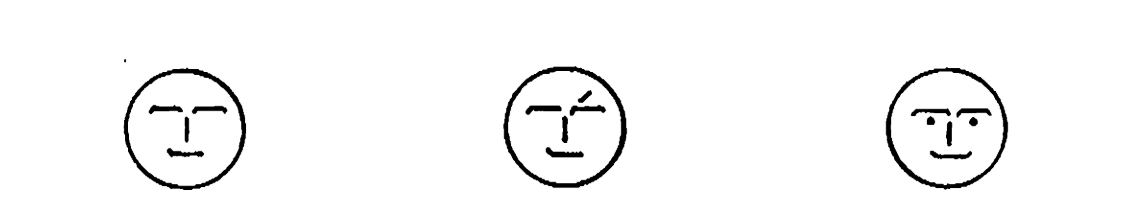
\includegraphics[width=\textwidth]{figures/introduction/faces.png}
    \caption{Faces}
    \label{fig:faces}
    \end{subfigure}
    \begin{subfigure}[b]{0.3\textwidth}
    \centering
    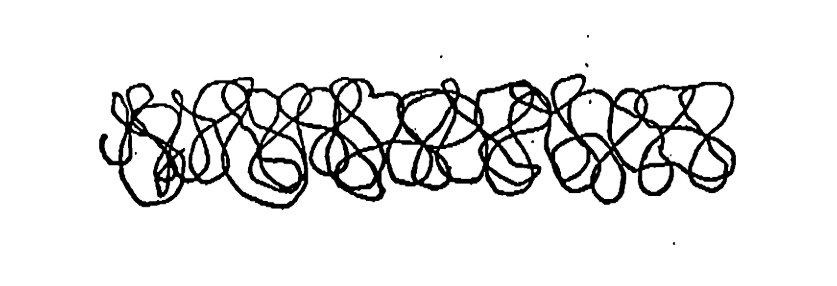
\includegraphics[width=\textwidth]{figures/introduction/squiggle_s.png}
    \caption{Squiggle S}
    \label{fig:squiggle}
    \end{subfigure}
    \caption{Left Faces, Right 'Squiggle S' \cite{Wittgenstien1967} }
    \label{fig:Witgenstein}
\end{figure}


\subsection{Empirical Aesthetics}

This domain covers a field of study within psychology and neuroscience where perception is studied using technologies such as eye tracking\cite{Younes2016} and leveraging environmental controls in experiments where subjects rank images. There is some overlap within the field of IAQA and its dataset, such as the Waterloo IAA\cite{Liu2017a}, where IAQA has used techniques normally applied within psychological experiments\footnote{A frequent critique of many IAQA datasets lack of control of ground truth data generation.}. 

\par

    %%%%%%
 %%%%%%%%%%%%%
   % %  % % 
       %    $$
     %%%%%

\begin{figure}[htp!]
\centering
\subfloat[Curve 2D Shape & Line]{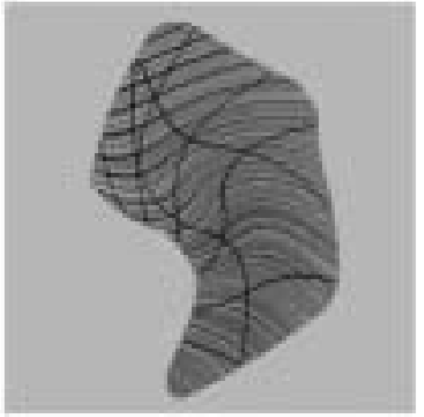
\includegraphics[width=0.15\textwidth]{figures/introduction/imperical aesthetics/curve.png}}
\subfloat[Non Curve 2D Shape & Line]{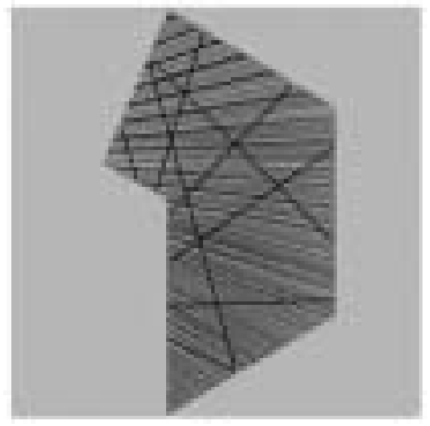
\includegraphics[width=0.15\textwidth]{figures/introduction/imperical aesthetics/non_curve.png}}
\subfloat[Curve Couch Design]{
  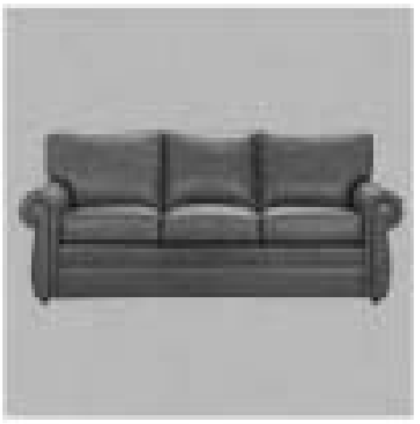
\includegraphics[width=0.15\textwidth]{figures/introduction/imperical aesthetics/curve_2.png}
}
\subfloat[Non-Curved Couch Design]{
  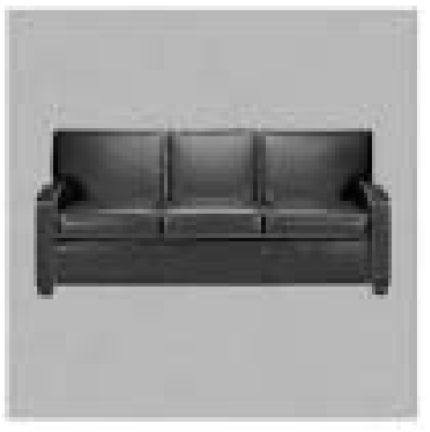
\includegraphics[width=0.15\textwidth]{figures/introduction/imperical aesthetics/non_curve_2.png}
 
}
\caption{Examples of Visual preference (a)(c) vs less pleasing (b)(d) \cite{Bar2006}}
\label{fig:curve}
\end{figure}

This is a relevant field, as it has provided  controls such as screen calibration, image display, subject demographic, and randomization of stimuli\cite{Leder2019,Mullennix2013, Rolls2014}. Empirical aesthetics also provides insight into areas such as visual symmetry, which are known to have also been a subject of computer vision\cite{Elawady2017,Gray2010}, and an understanding of how viewers might rank an image. 
\begin{figure}[H]
\centering
\subfloat[Random Image]{
  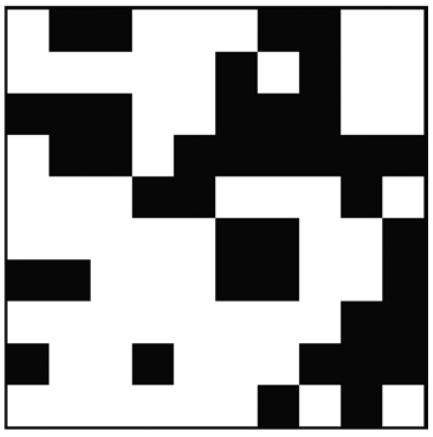
\includegraphics[height=0.15\textwidth]{figures/introduction/imperical aesthetics/random_1.png}
  \label{fig:non_symetry}}
\subfloat[Symmetrical Image]{
  
\includegraphics[height=0.15\textwidth]{figures/introduction/imperical aesthetics/symetry.png}
  \label{fig:symetry_reflect}}
\subfloat[Rotational Symmetry Image]{
  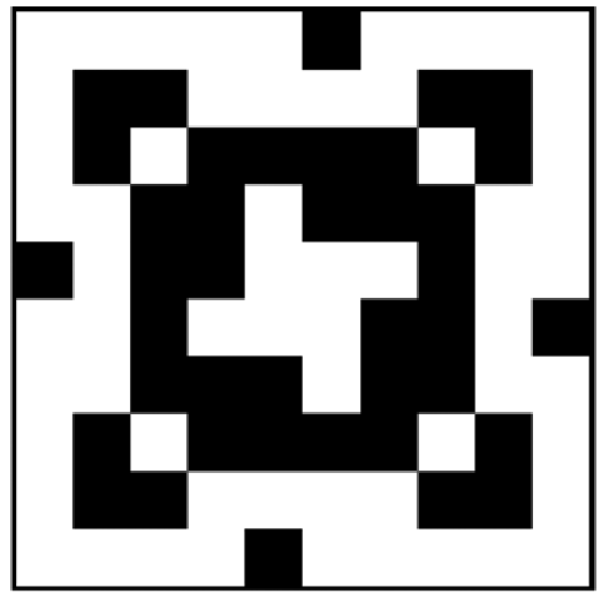
\includegraphics[height=0.15\textwidth]{figures/introduction/imperical aesthetics/rotational_symetry.png}
  \label{fig:symetry_rotation}}
\caption{Examples of images used in psychological experiments showing visual preference for symmetry and complexity      \cite{Bertamini2013}}
\label{fig:symetry}
\end{figure}


These studies have shown experimentally both that formal rules such as the 'golden ratio' and 'averageness' in facial portraits (figure \ref{fig:means}), symmetry (figure \ref{fig:symetry}), complexity\cite{Bertamini2013}, and curve (figure \ref{fig:curve}) are attributes that are associated with aesthetically pleasing design and images (figure \ref{fig:means}).

\begin{figure}[ht!]
    \centering
    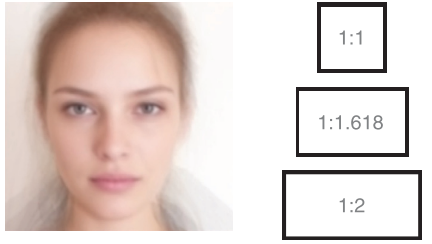
\includegraphics[width=0.3\textwidth]{figures/introduction/imperical aesthetics/means.png}
    \caption{Average Composite Face (left) , Golden Ratio (Middle Right) \cite{Brielmann2018}}
    \label{fig:means}
\end{figure}

\par

However, this is far from the whole `picture' and it has been shown both in computer vision \cite{Simond2015} and in imperial aesthetics publications alike that attributes such the golden ratio or rule of thirds in photography\cite{Green2012} and symmetry\cite{Leder2019} are not universal aesthetic attributes and depend on context - this underscores the complex nature inherent within the domain of aesthetics. 



\subsection{Art Aesthetics}

Art aesthetics and criticism include consideration of brush strokes and artist techniques, alongside the interpretation of images within cultural and critical studies that intersect with social sciences, literary criticisms and philosophy. \textit{Perspectives} within art aesthetics might consider or include \textit{Marxist, psychoanalytical, feminist (figure \ref{fig:femnist_art}) and queer (figure \ref{fig:mapplethorp}}). 

\par The tradition in the 20th century has been to apply intellectual theory that has also been applied to other art forms, such as film and literature, and is not limited to considerations of \textit{good} or \textit{bad} opinion but rather critical and conceptual analysis using vernacular such as `feminist aesthetics' or `feminist critique'\cite{Hein1990} of an artwork, item of popular culture or an image.

\par One fascinating feature of 20th century art is the inclusion of critical theory into the artwork aesthetics itself and `aesthetics' that are ironic or a pastiche of popular culture's aesthetics (figure \ref{fig:femnist_art} shows two renowned and striking examples of this). 
\begin{figure}[htp!]
\FloatBarrier
    \centering
    \subfloat[ (sic.) Untitled (Your Body is a Battleground)\footnote{Untitled is used ironically with inclusion of parenthetic title} \cite{Kruger1898}]{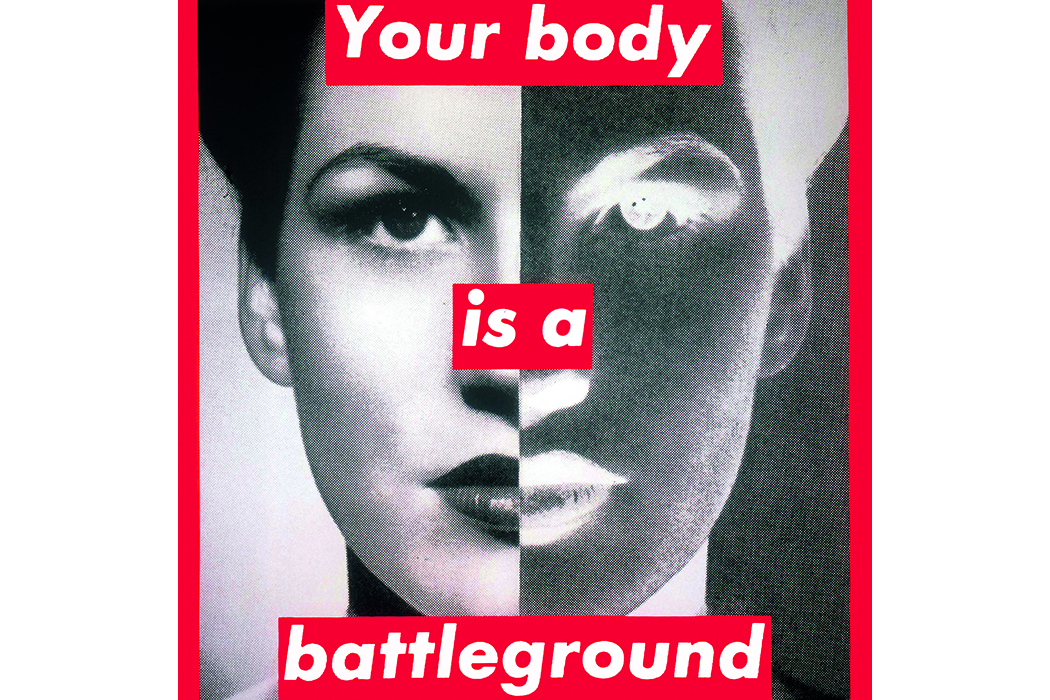
\includegraphics[height=0.2\textwidth]{figures/introduction/art aesthetics/Kruger_1050x700.jpg}}
    \hfill
    \subfloat[Do Women Have To Be Naked To Get Into the Met. Museum?\    \cite{TheGorillaGirls1989}]{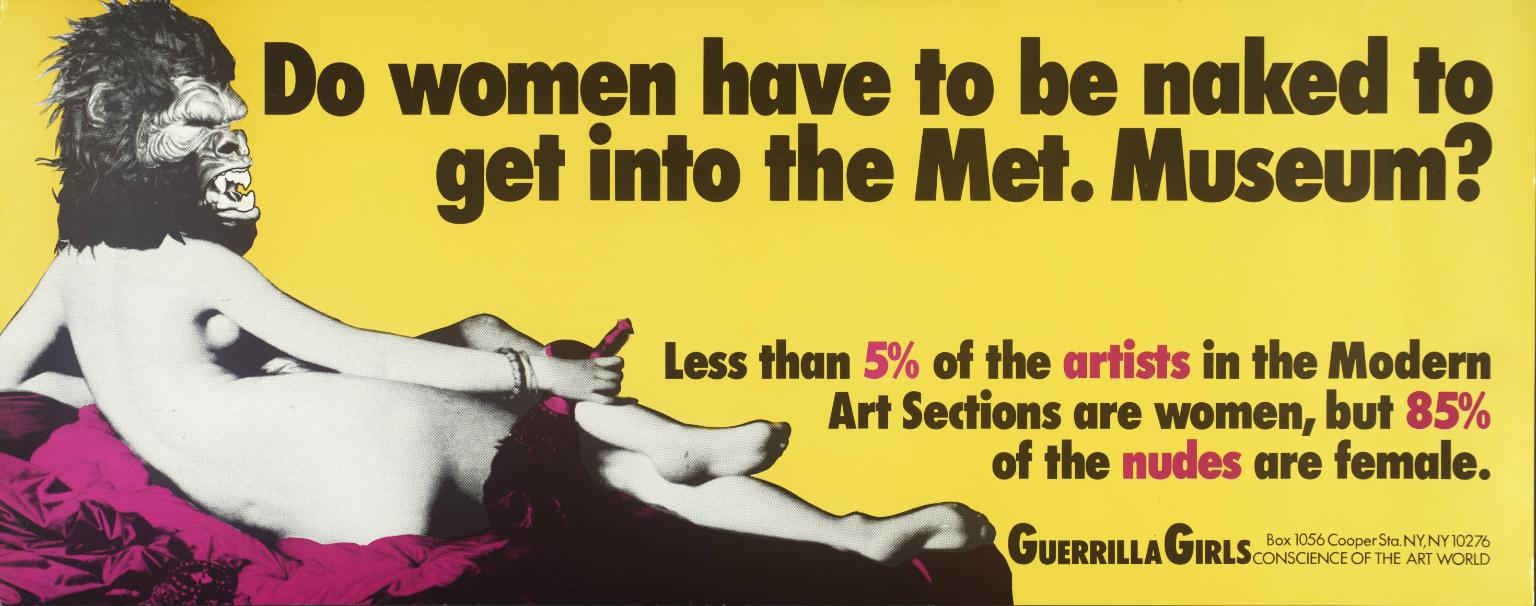
\includegraphics[height=0.2\textwidth]{figures/introduction/art aesthetics/gorrilla girls.jpg}}
    \caption{Examples of Late 20th century Feminist Artworks}
    \label{fig:femnist_art}
\end{figure}
\par Art aesthetics this are important and relevant in considering the possible applications of IAQA and given how different models that are trained apparently handle ambiguous examples and the potential to provide a `critical lens' on areas such as cultural, racial or gender bias that might be replicated by machines. One might ask here how computer vision might learn feminist aesthetics?

\par Much of the focus of IAQA has been on what might fall within extraction of features: formalist art aesthetics, such as lighting, perspective or particular aesthetic techniques such as chiaroscuro (using lighter or darker tonal values to make something appear three dimensional)\cite{Hobbs1990} shown in \ref{fig:chiaroscuro}. 
\par Another example of formalist aesthetics involves using attributes such as colour harmony - or using colours that are equidistant on a colour wheel (figure \ref{fig:colorwheel}) - which positions discrete colours according to position, following prismatic splitting (figure \ref{fig:newton}) (or electromagnetic spectrum) first theorized by Newton \textit{red, orange, yellow, green, blue, indigo, violet}.

\begin{figure}[ht!]
\centering
    \subfloat[Self Portrait by Artist Robert Mapplethorpe    \cite{Mapplthorpe1980}]{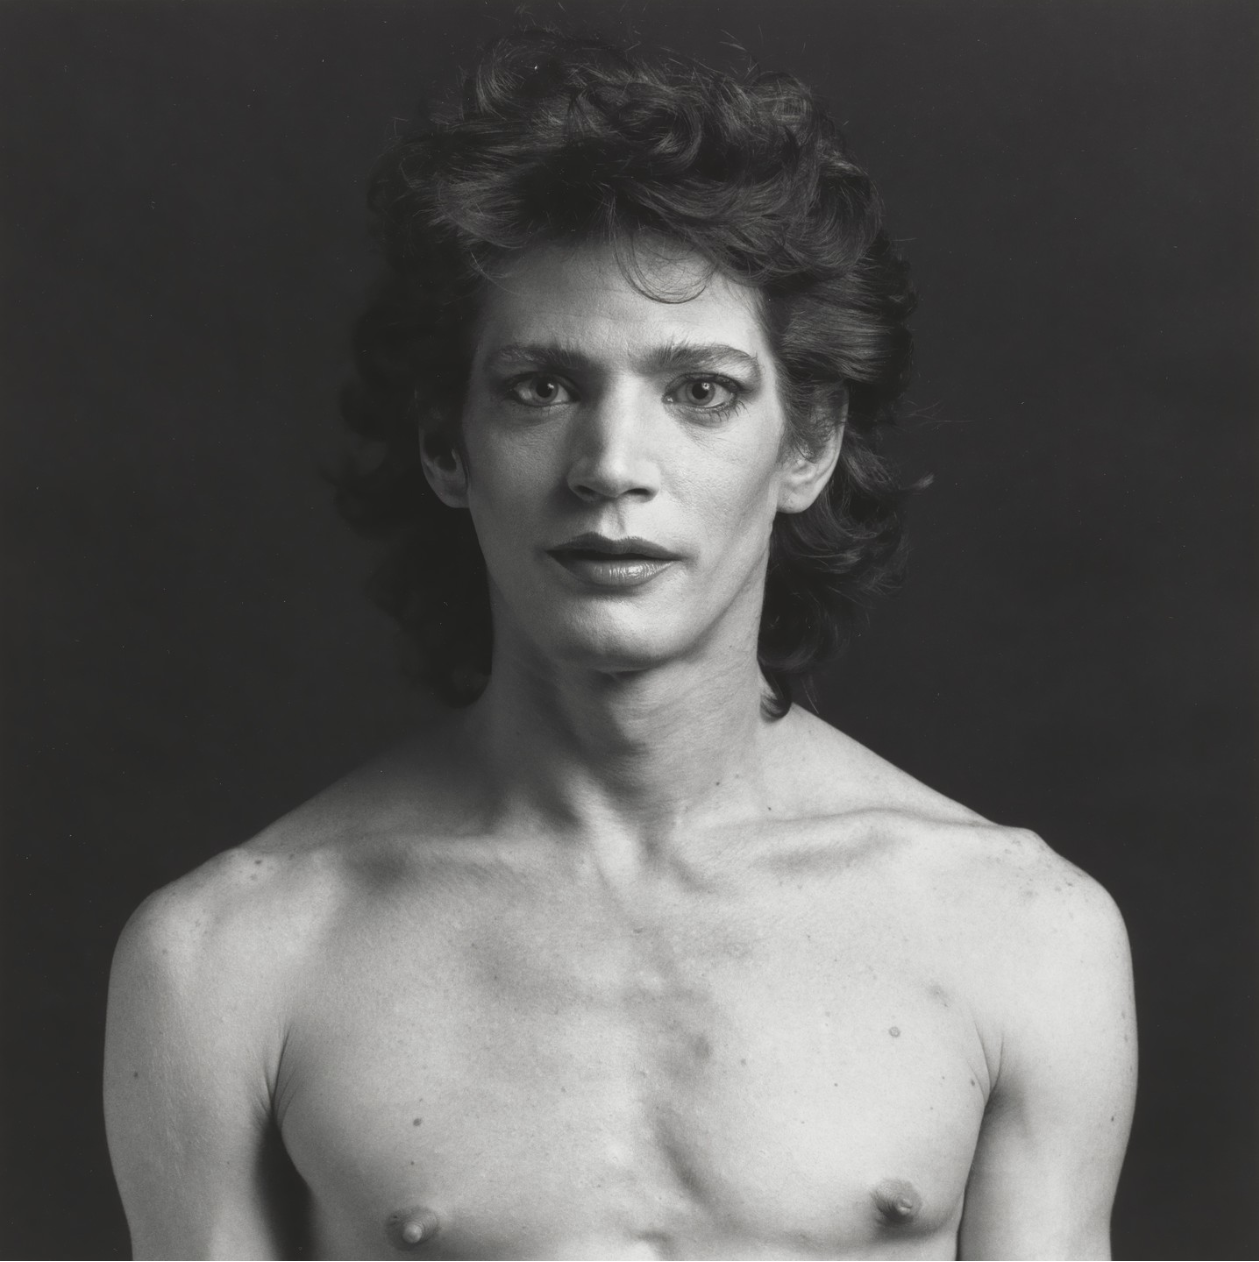
\includegraphics[width=0.2\textwidth]{figures/introduction/art aesthetics/mapplthorp.png}
    \label{fig:mapplethorp}}
    \hfill
    \subfloat[El Fabula(an Alegory) \cite{Domenikos1580}]{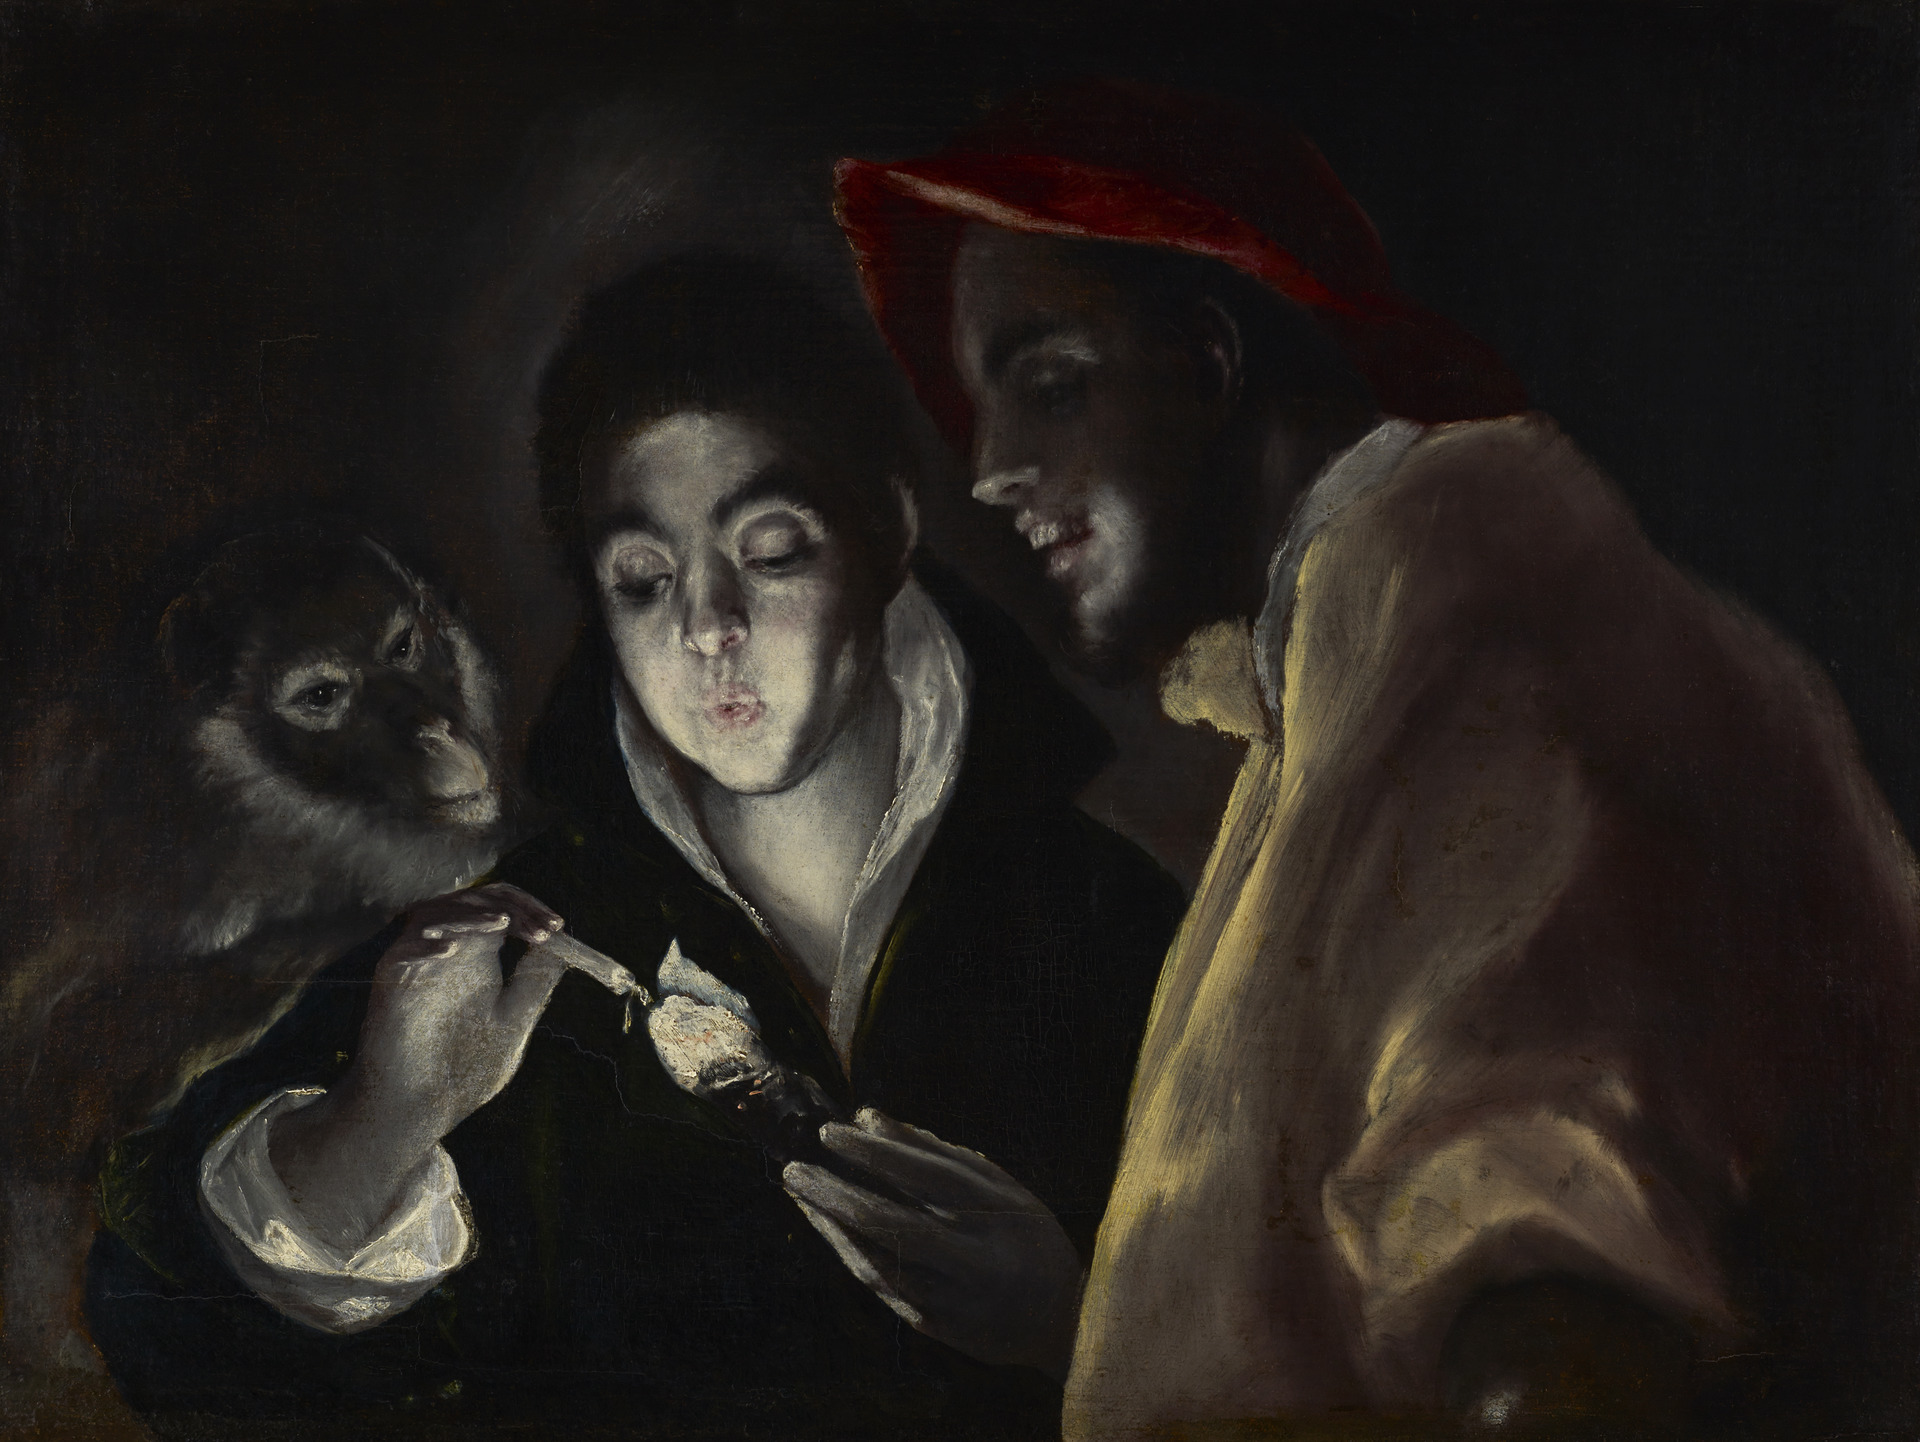
\includegraphics[width=0.2\textwidth]{figures/introduction/art aesthetics/an-allegory-f-bula.jpg}}
    \hfill
    \subfloat[Salome Receives the Head of John the Baptist   \cite{Caravaggio1609}]{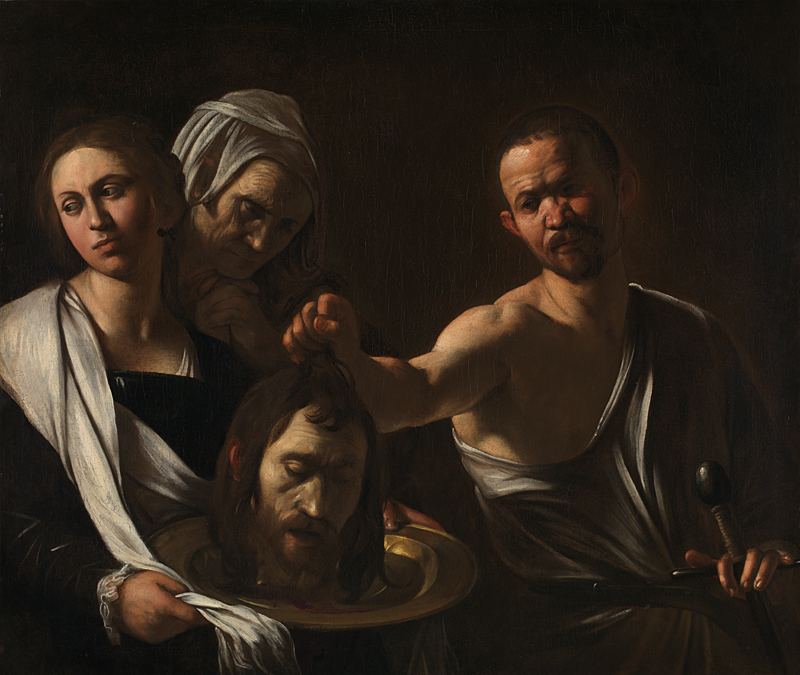
\includegraphics[width=0.2\textwidth]{figures/introduction/art aesthetics/carrivagio.jpg}}
    \caption{Chiaroscuro examples}
    \label{fig:chiaroscuro}
    \vfill 
    \subfloat[ Newton's Color Wheel Based on EMS (Prismatic Splitting)]{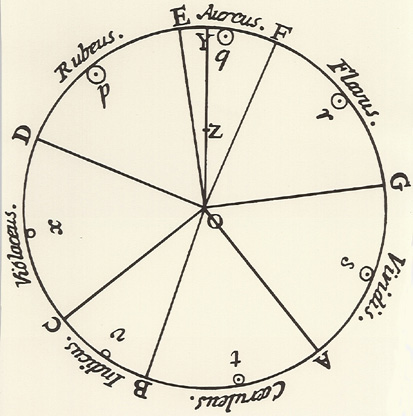
\includegraphics[width=0.2\textwidth]{figures/introduction/art aesthetics/Newton-Color-wheel.jpg}
    \label{fig:newton}}
    \hfill
    \subfloat[Primary and Secondary Hues in Pigments  \cite{Hobbs1990}]{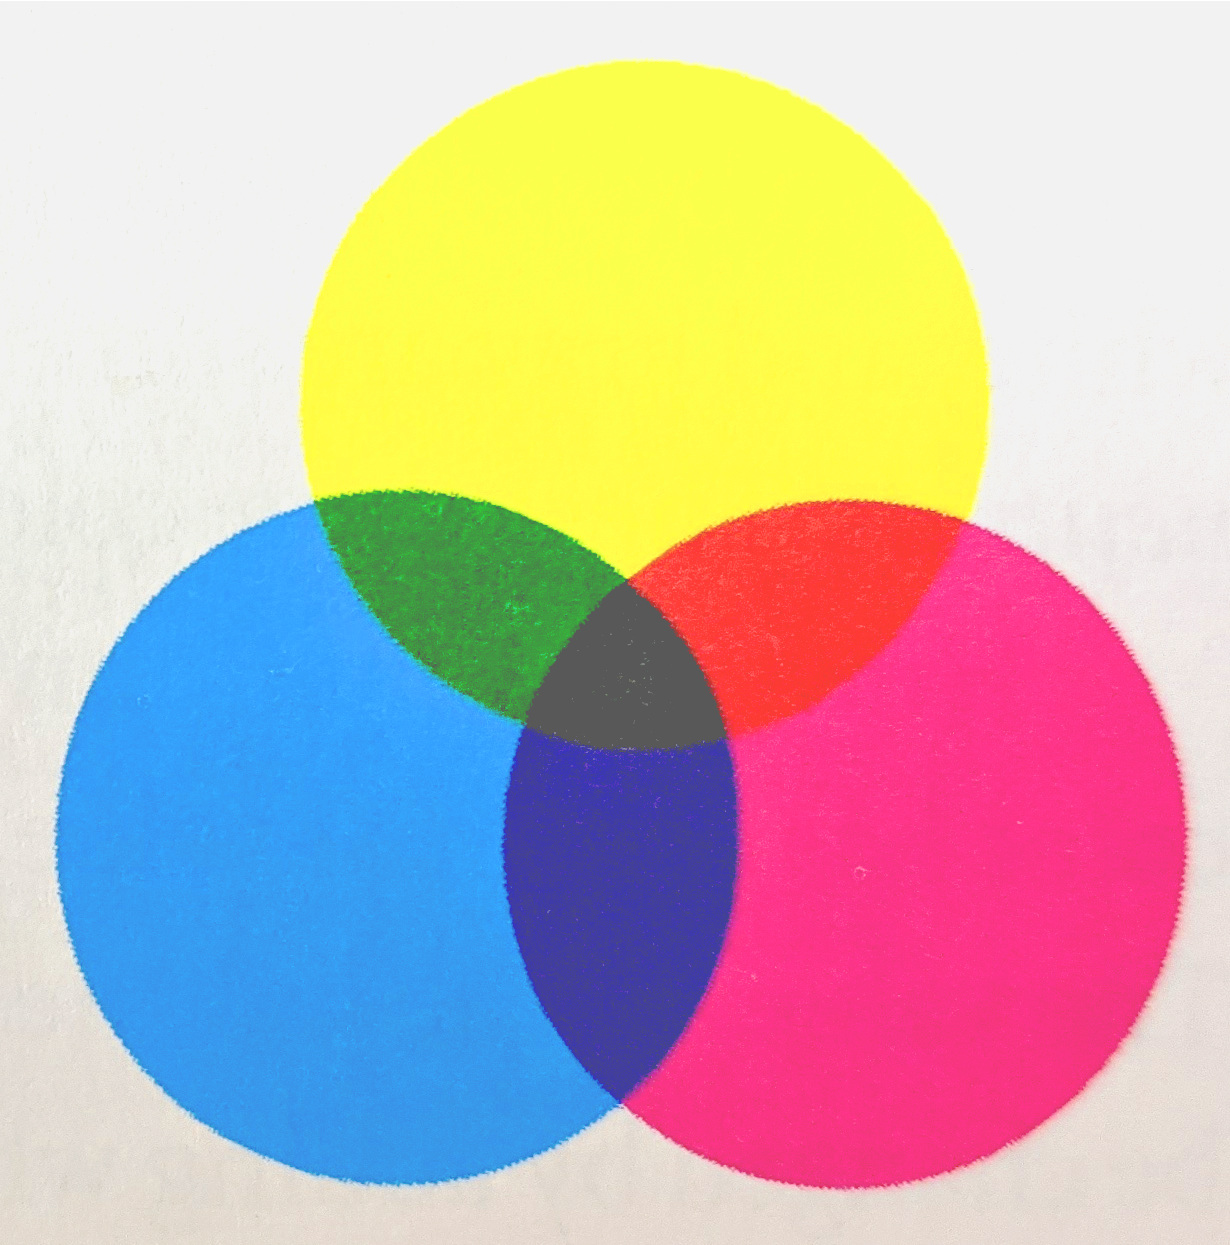
\includegraphics[width=0.2\textwidth]{figures/introduction/art aesthetics/chromatic_splitting.jpg}}
    \hfill
    \subfloat[ Aesthetics Color Wheel   \cite{Hobbs1990}]{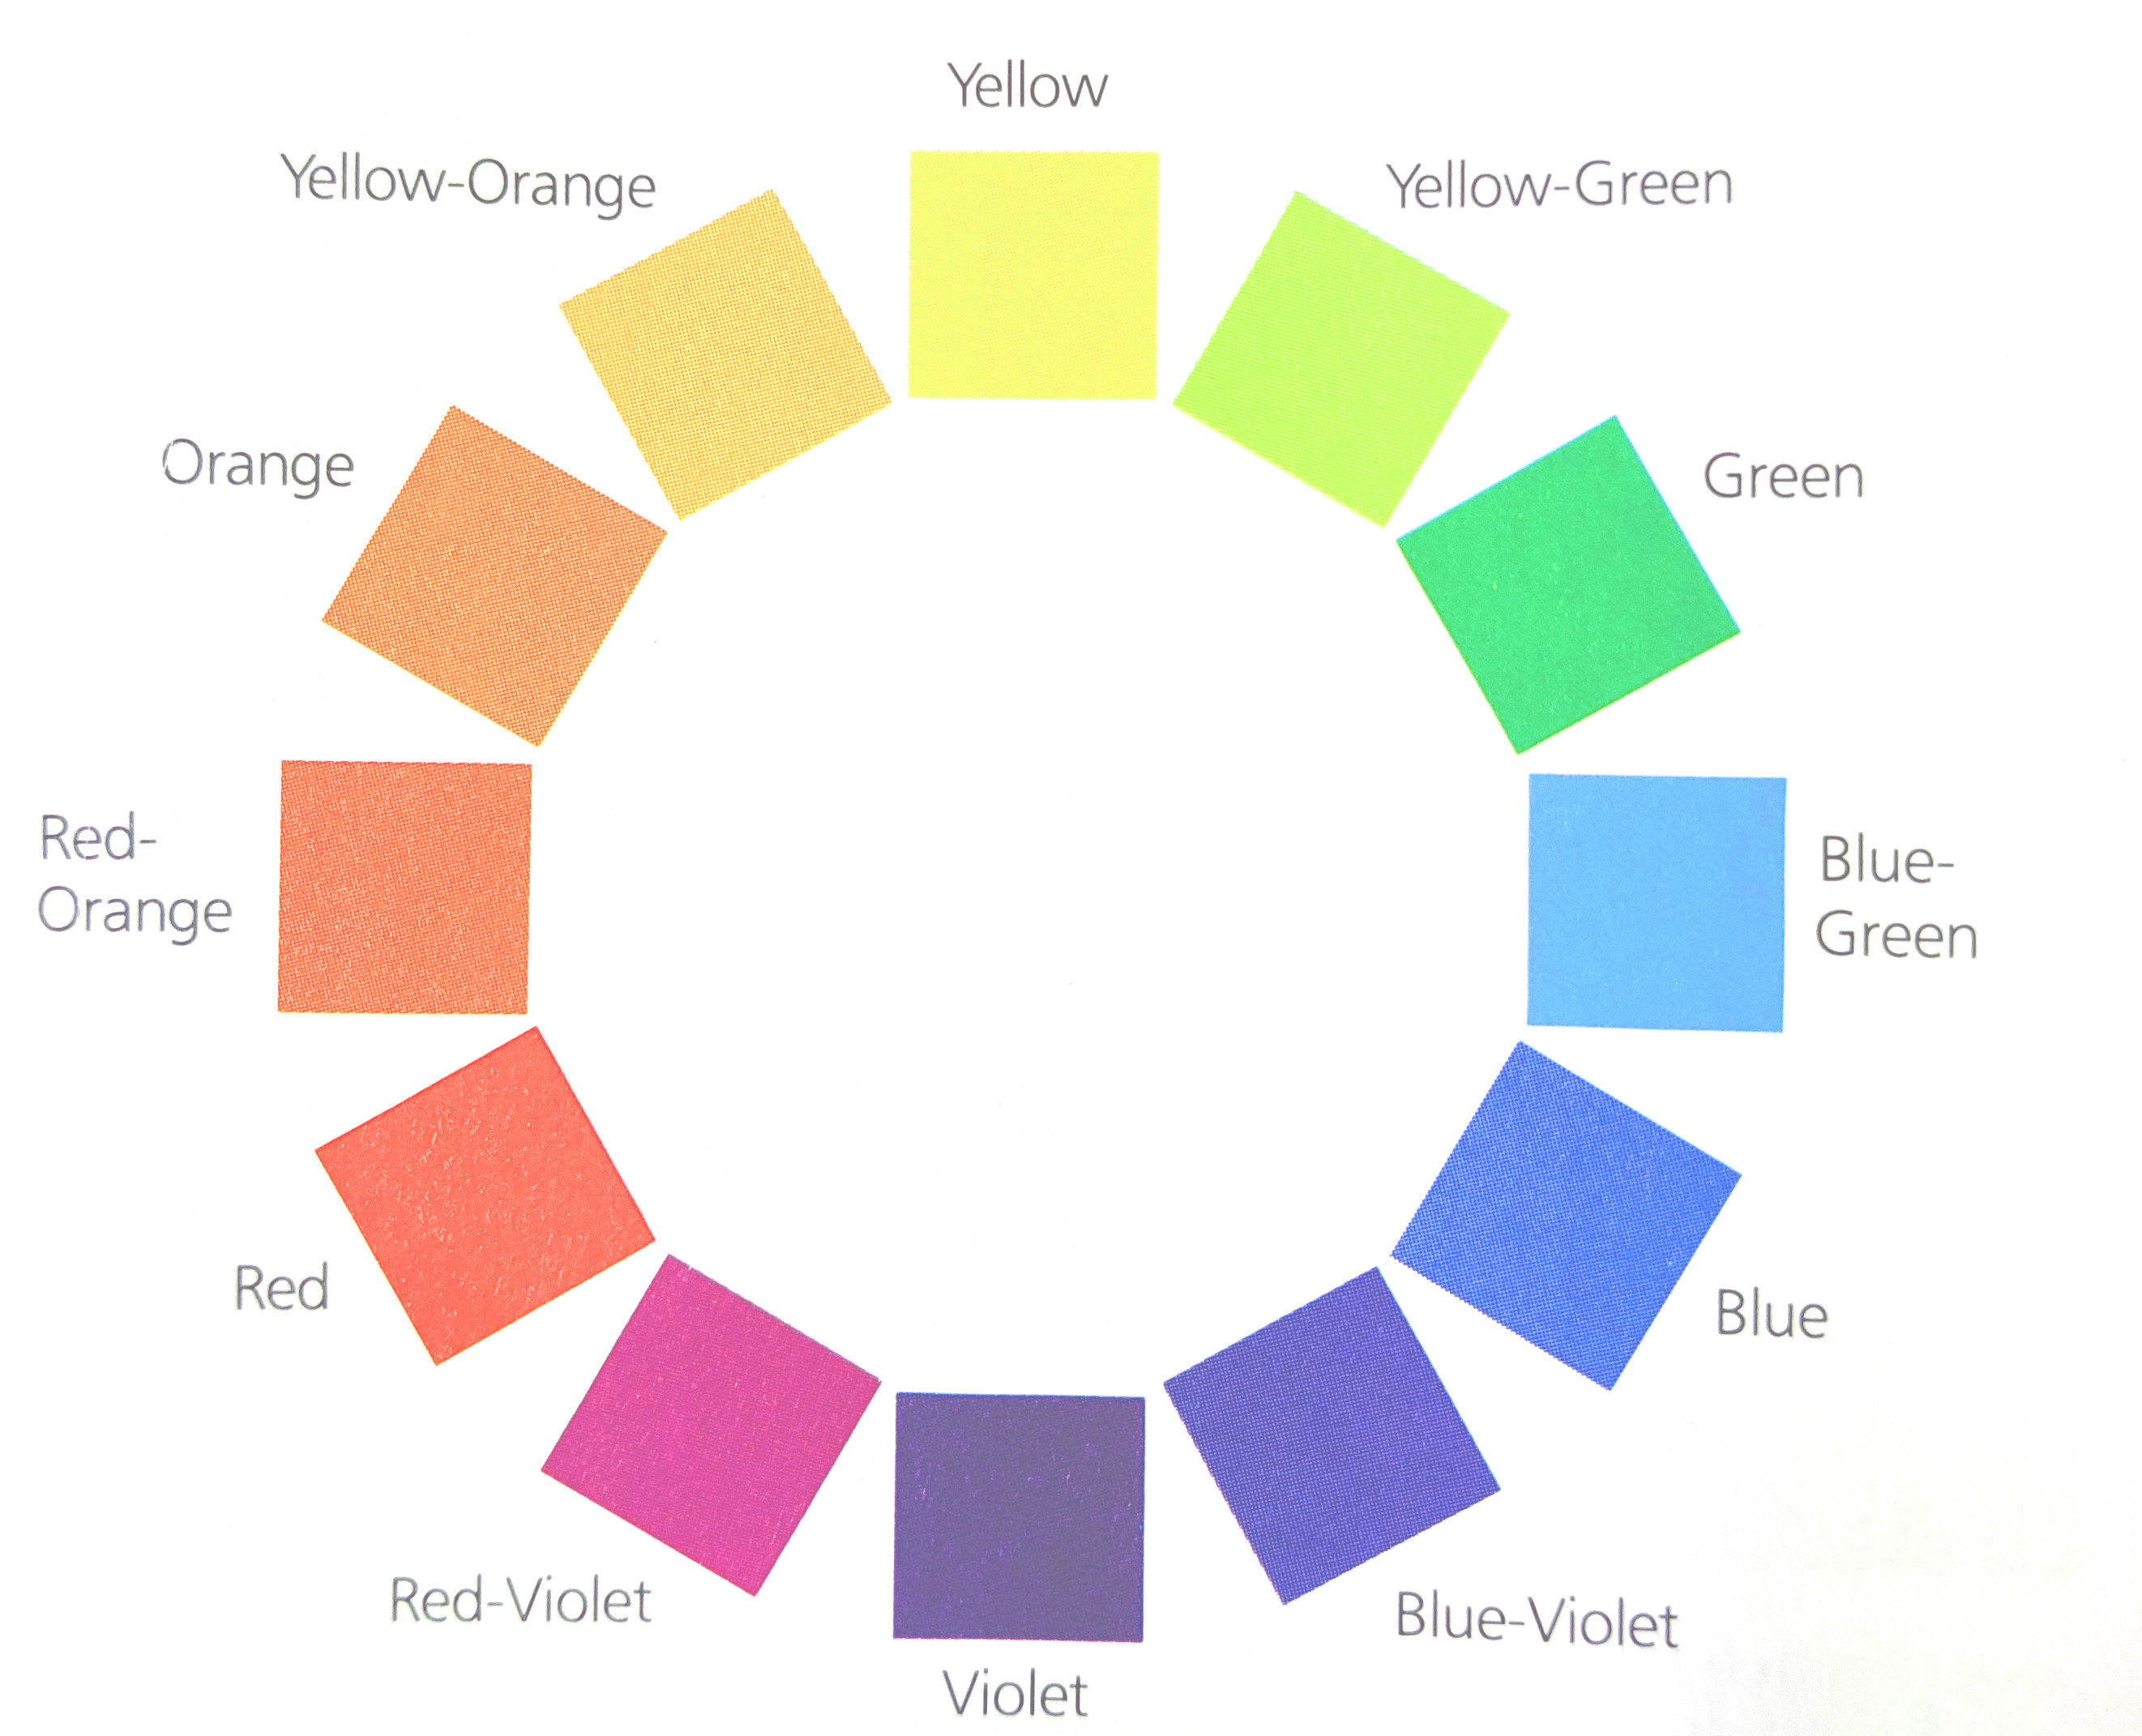
\includegraphics[width=0.2\textwidth]{figures/introduction/art aesthetics/colour_wheel.jpg}}
    \caption{Examples of Colour}
    \label{fig:colorwheel}
\end{figure}

Many formalist attributes are used in hand crafted IAQA, and a consideration to wider aesthetics is included as there may be novel applications of computer vision to art criticism. One such high-level example of formal aesthetics is shown in figure \ref{fig:elements of design}; a focused example of features in IAQA literature is shown in table \ref{tab:aes_attribs}.

\begin{figure}[h!]
    \centering
    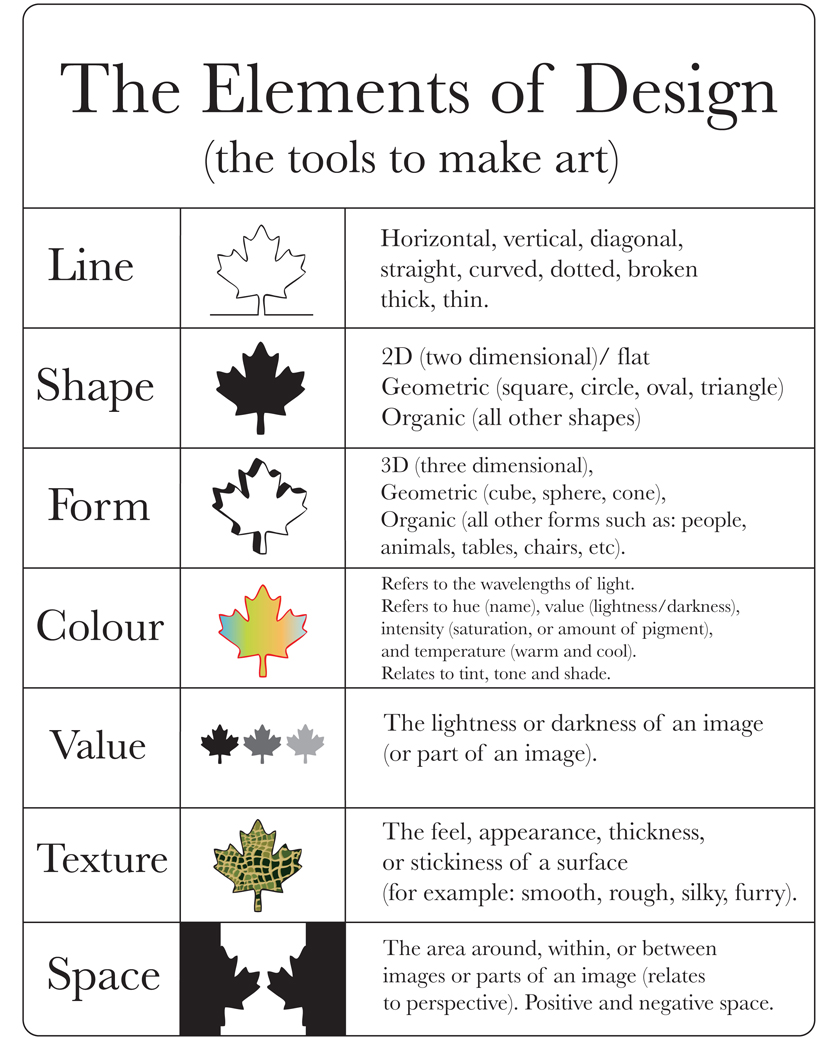
\includegraphics[height=0.4\textwidth]{figures/introduction/art aesthetics/elements3.jpg}
    \caption{Elements of Design \cite{Butler2012}}
    \label{fig:elements of design}
\end{figure}

\subsection{Photo Aesthetics}

Photographic aesthetics within the field of IAQA have focused on so-called 'formal photographic rules', which overlap with more widely applied aesthetic rules, but have distinct properties which are a result of physical properties: lens (bokeh, Depth of Field(DOF), shutter speed), sensor, and light. Within traditional handcrafted approaches, this involved high-level attributes such as \textit{simplicity, colourfulness, color combination(harmony), sharpness, image pattern, and object composition}\cite{Liu2017a,Mavridaki2015,Datta2006,Tang2013a,Simond2015,Lo2013}. These are informed by texts on photography that themselves frequently borrow from formalist art aesthetics, which have, in turn, been sources from which high-level features are defined. 

\begin{figure}[ht!]
\centering
    \subfloat[Complimentary Colors(Color Contrast) Yellow/Blue  \cite{Ke2006}]{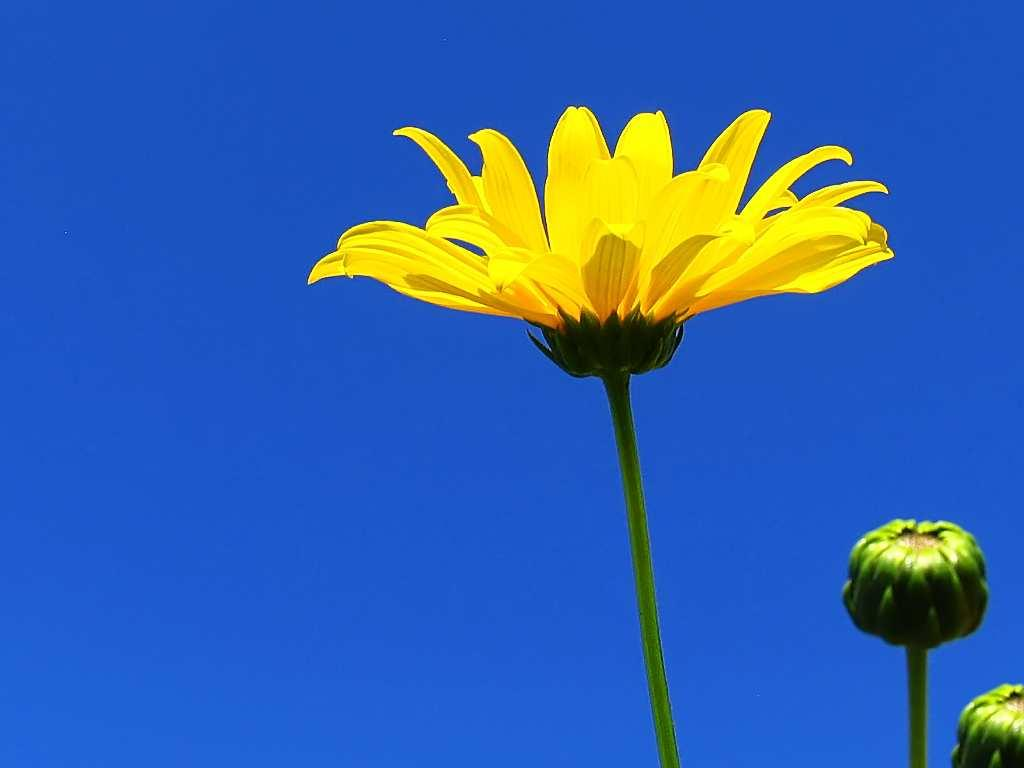
\includegraphics[width=0.2\textwidth]{figures/introduction/photo aesthetics/flower_contrast.jpg} \label{fig:colour contrast}}
    \hfill
     \subfloat[ Colour Harmony \cite{Lo2013}]{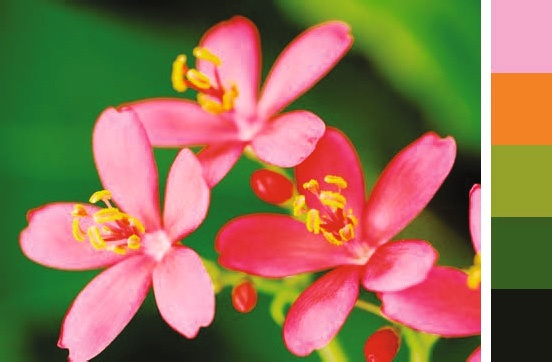
\includegraphics[width=0.2\textwidth]{figures/introduction/photo aesthetics/harmony.jpeg}
     \label{fig:harmony}}
     \hfill
     \subfloat[ Shutter Speed \cite{Lo2013}]{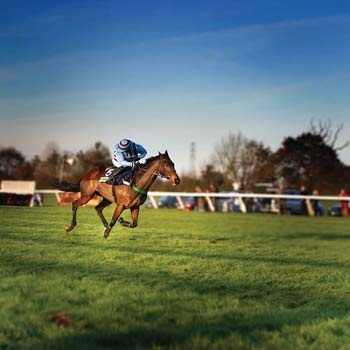
\includegraphics[height=0.15\textwidth]{figures/introduction/photo aesthetics/shutter speed.jpeg}
     \label{fig:shutter speed}}
    \vfill
    \subfloat[Rule of thirds \cite{Mai2011a}]{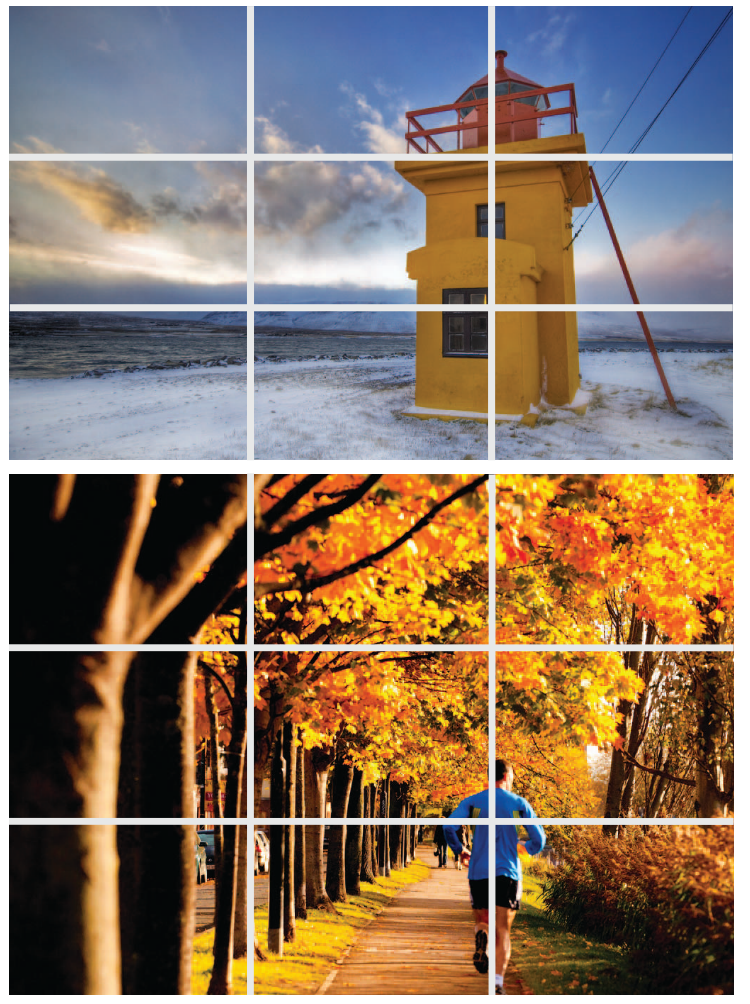
\includegraphics[height=0.2\textwidth]{figures/introduction/photo aesthetics/rule of thirds.png}
    \label{fig:composition}}
    \hfill
    \subfloat[Shallow Depth of Field (Blurring Background) \cite{Ke2006}]{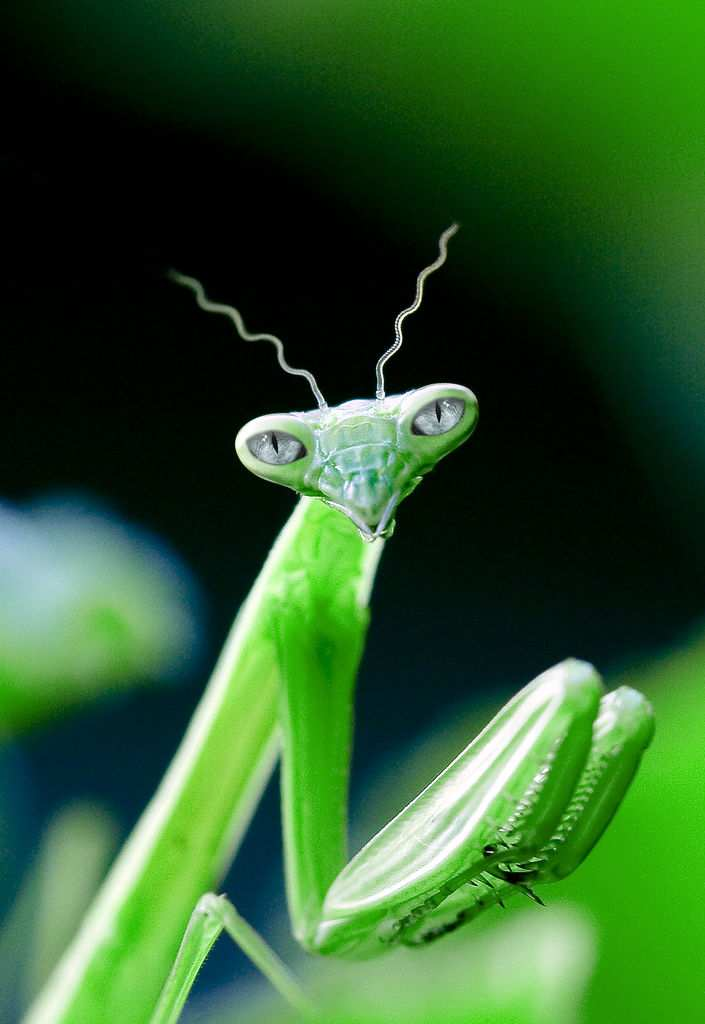
\includegraphics[height=0.2\textwidth]{figures/introduction/photo aesthetics/Look Intoby Josh Brown.png}\label{fig:object emphasis}}
    \hfill
    \subfloat[Good Lighting \cite{Lo2013}]{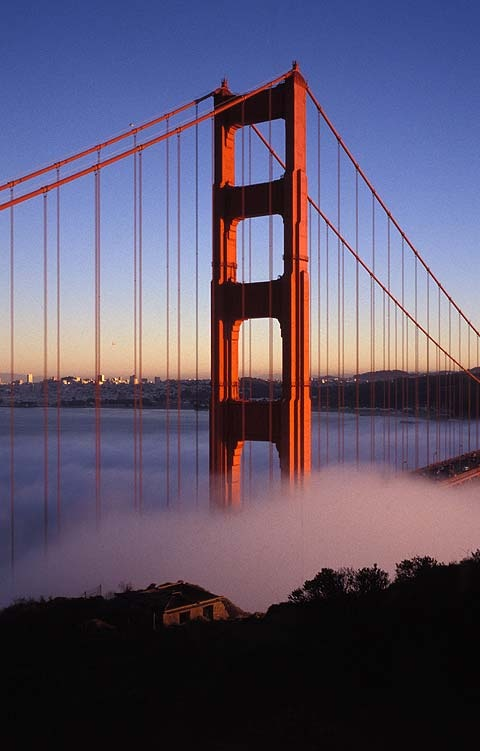
\includegraphics[height=0.2\textwidth]{figures/introduction/photo aesthetics/good_lightin.jpeg} \label{fig:lighting}}
    \caption{Examples of Photographic Formal Aesthetics}
    \label{fig:attr}

\end{figure}


Others have sought to define more abstract features, such as spatial richness\cite{Lo2013} and similarity measure\cite{Datta2006}; aesthetic attributes that are concepts of a hypothetical viewer mapped onto ranking measures. Table \ref{tab:aes_attribs} shows attributes frequently used in IAQA literature, many of which are defined within photographic texts, photo guides or researchers' own experience. It is also clear from, for instance, attributes like \textit{good lighting} are not necessarily easy to define though they may appear obvious, and that these include detailed aspects such as chiaroscuro, dynamic range, and contrast. 

\par Further, these attributes are not strictly cumulative and/or necessarily combinatorial - attributes that may constitute a \textit{good} photograph for one subject would not necessarily be effective should the subject be elsewhere. There are numerous examples of this in the datasets section of the appendix  \ref{iaqa datsets appendix}. 

\par However, it is also clear that having an intuition as a photographer is part of the aesthetic toolkit, and a re-combinatorial approach - using the right effects alongside the adjustment of camera settings, lense choice - is a part of what makes 'good photography'.

\par Figure \ref{fig:composition} bottom clearly has \textit{rhythm, colour harmony, composition} created by the object of the photograph being at the intersection of the golden ratio, the colour of the leaves, the repetition of trees and it also makes use of perspective - an image figure \ref{fig:lighting} shallow DOF(wide lens iris aperture/low $f$ number)  would be not be a useful attribute and would render the bridge out of focus. Attributes such as shallow DOF that in one context (portraiture or macro photography) are part of highlighting a salient object that in another (landscape photography) would degrade the image aesthetics quality\footnote{$f$ 64 is a renowned landscape movement which makes use of extremely small apertures-rendering almost everything in focus to create a painterly quality of image, examples of this can be seen on the Metropolitan Museum of Art's web-page:  \href{https://www.metmuseum.org/toah/hd/f64/hd_f64.htm}{https://www.metmuseum.org/toah/hd/\f64/hd\_f64.htm}}. Many of the low quality images in the qualitative examples of IAQA datasets (section \ref{iaqa datsets appendix} of the appendix) show images that might otherwise be high quality but the image has of shallow DOF with a salient object that is out of focus.

\begin{table}[t]
\centering
\small 
\begin{tabular}{p{0.2\textwidth}<{\centering}?cp{0.5\textwidth}}
\specialrule{0.1em}{0.1em}{0.1em}
 \multicolumn{3}{c}{Example Aesthetic Attributes}\\
 \specialrule{0.1em}{0.1em}{0.1em}
  \textbf{Feature(aesthetic Attribute)}  & \textbf{Figure} & \textbf{Description}\\
  \specialrule{0.1em}{0.1em}{0.1em}
  Rule of Thirds/ Object Composition & \textbf{\ref{fig:composition}} & Salient or important elements placed on lines of image divided into $3\times3$ grid. Ratio of $1.61803$ \cite{Yeh2012}\\
  
  \specialrule{0.05em}{0.1em}{0.1em}
  Saturation/ Hue Saturation &\textbf{\ref{fig:colour contrast}} & saturation indicate chromatic purity (emphasis of single color value) \cite{Datta2006} \\
  
  \specialrule{0.05em}{0.1em}{0.1em}
  Simplicity &\textbf{\ref{fig:colour contrast}} & Keeping single subject or saline object well composes and not having too many subjects in frame.\cite{Tang2013a}\\
  
  \specialrule{0.05em}{0.1em}{0.1em}
  Color Combination & \textbf{\ref{fig:harmony}} & Color Distribution of image finding a few dominant colours\cite{Lo2013,Tang2013a}\\
  
  \specialrule{0.05em}{0.1em}{0.1em}
  Lighting & \textbf{\ref{fig:lighting}} & lighting contrast between foreground and background, use of effects such contrast\cite{Kong2016, Lo2013}\\
  
  \specialrule{0.05em}{0.1em}{0.1em}
  Sharpness & \textbf{\ref{fig:object emphasis}} \ & Subject in focus, use of depth of field and lighting to isolate salient object from background\cite{Mavridaki2015a}\\
  
  \specialrule{0.05em}{0.1em}{0.1em}
  Image Pattern & \textbf{\ref{fig:composition} bottom}& Use of symmetry and texture to crate harmony and rhythm\cite{Mavridaki2015a,Kanwal2021}\\
  \specialrule{0.1em}{0.1em}{0.1em}
\end{tabular}
\caption{ Aesthetic Attributes from IAQA Literature}
\label{tab:aes_attribs}
\end{table}


One further aspect of photo aesthetics that is important to consider is the properties of the camera, this might include resolution of sensor, bit depth of color, alongside the sharpness of lens which effects both features such as chromatic aberrations (red, blue halo at object edge) and resolving power of lenses, many of these properties are interrelated. For instance small $f$ number (aperture) increase sharpness even for low quality lenses but also increase DOF. Other aspects include tilt and shift (figure \ref{fig:tilt shift all egs}) where a specialist lens or large format camera might be used in architecture photography to correct perspective. 



\newpage    
\section{Applications}


\subsection{Commercial Applications and Practical Applications}

Applications include image recommendation, photo album optimisation\cite{Liu2017} and advertising, alongside image enhancement\cite{Talebi2018} and on-device real time IAQA. Others have utilised image captioned ground truth to train models that have then been able to offer advice to photographers, providing feedback on aspects of technique and camera operation such as,\textit{`a greater depth of field of say f8 would have produced an over all better shot'}\cite{Jin2019}, these latter approaches have also made use of attributes' radar maps\cite{Jin2019}. Another related approach is 'best hand shot'\cite{Schwarz2018a} which utilises the multi-capture feature that many smart phones are now equipped with.

\begin{figure}[ht!]
    \centering
    \subfloat[Image Before Enhancement Enhancement\cite{Talebi2018}]{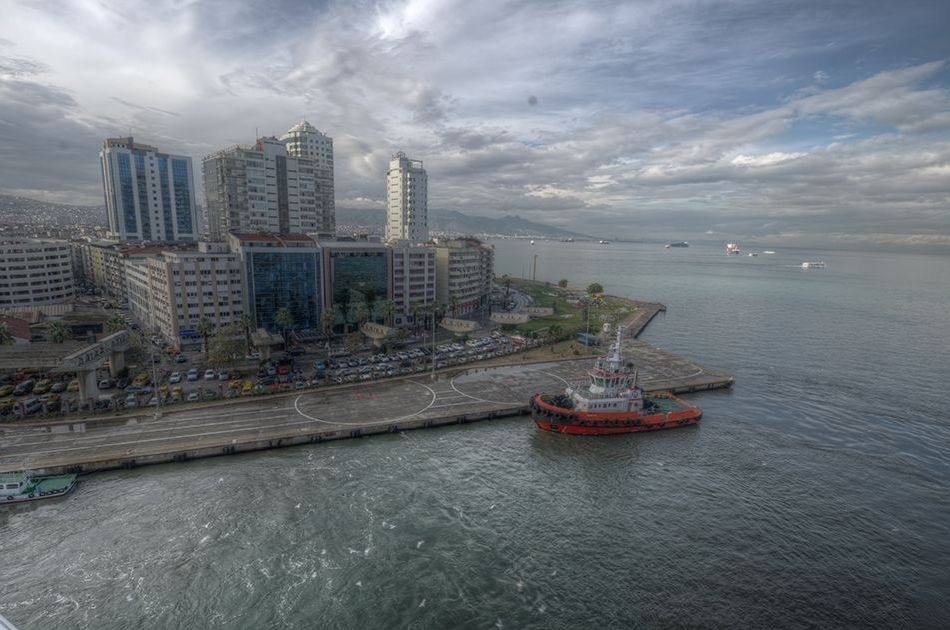
\includegraphics[width=0.2\textwidth]{figures/introduction/examples of applications/11Talebi, Milanfar - 2018 - NIMA Neural Image Assessment-annotated.pdf1.jpeg}}
    \vspace{3mm}
    \subfloat[Image Before Enhancement\cite{Aydin2015}]{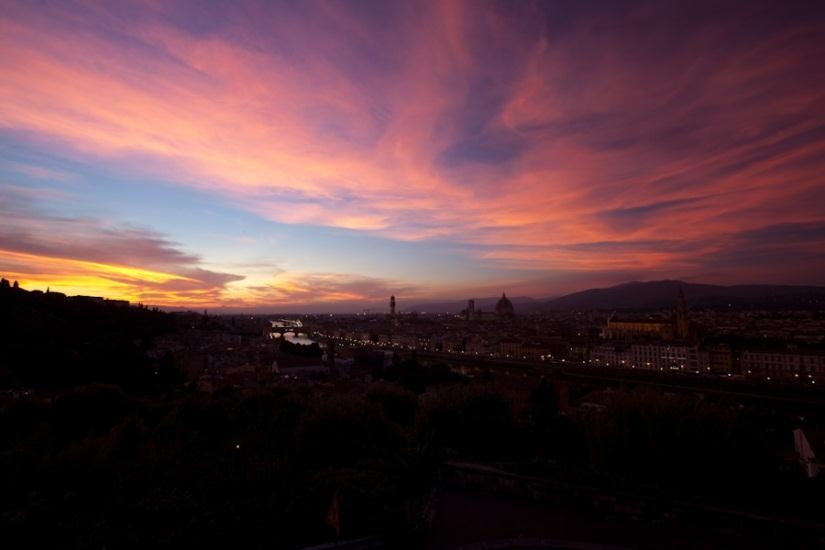
\includegraphics[width=0.2\textwidth]{figures/introduction/examples of applications/1Automated Aesthetic Analysis.pdf1.jpeg}}
    \vspace{3mm}
     \subfloat[Image Before Automatic Crop Enhancement\cite{Schifanella2015}]{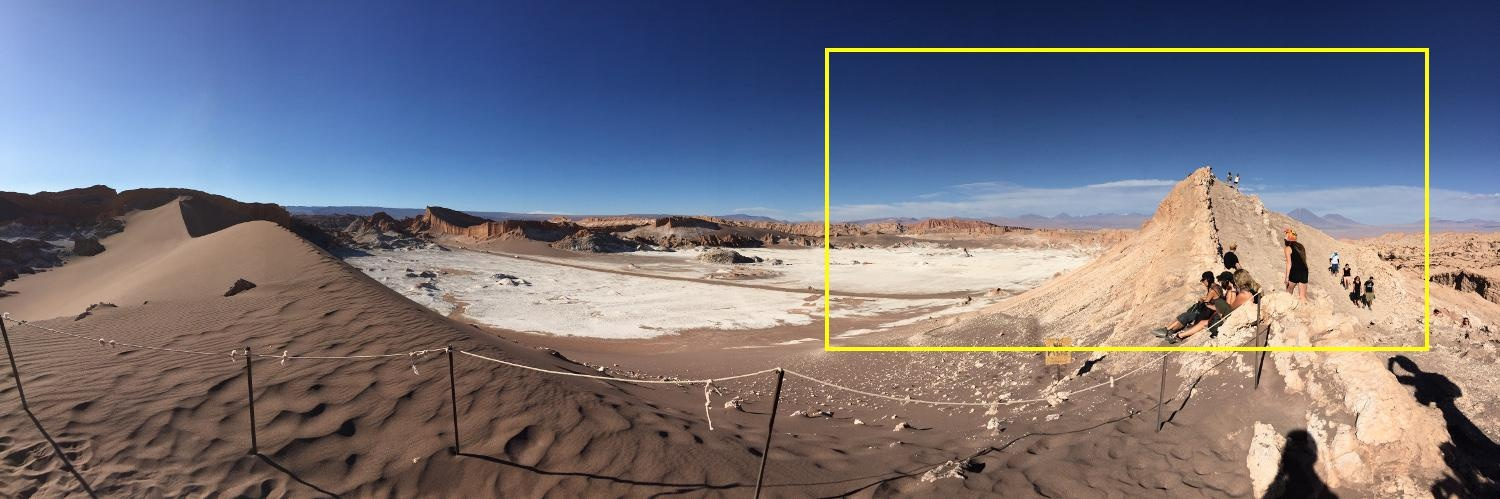
\includegraphics[width=0.2\textwidth]{figures/introduction/examples of applications/7Learning to Compose with Professional Photographs on the Web.pdf5.jpeg}}
    \vfill 
    \subfloat[Image After Enhancement Enhancement\cite{Talebi2018}]{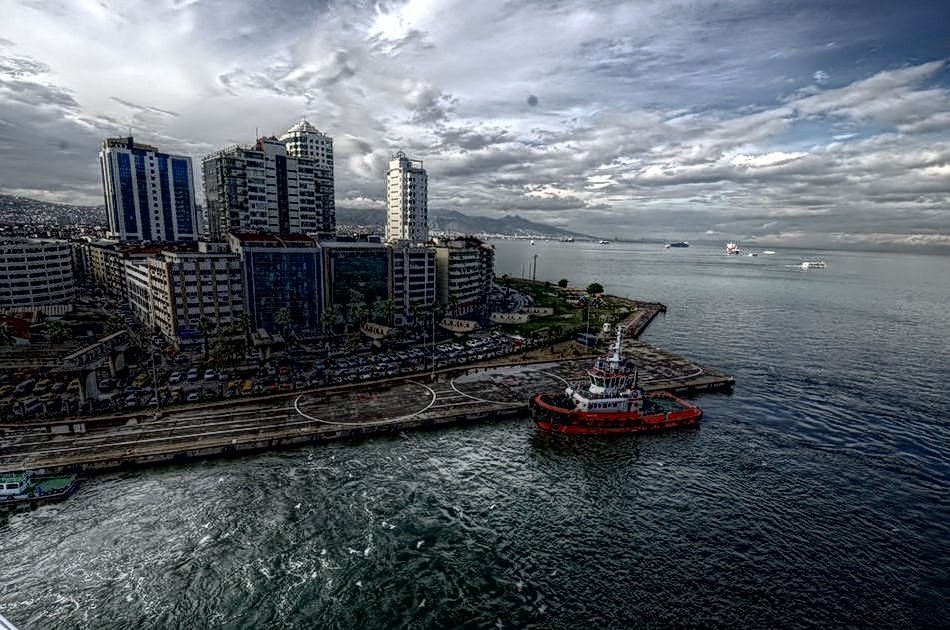
\includegraphics[width=0.2\textwidth]{figures/introduction/examples of applications/11Talebi, Milanfar - 2018 - NIMA Neural Image Assessment-annotated.pdf2.jpeg}}
    \vspace{3mm}
    \subfloat[Image After Enhancement  Enhancement\cite{Aydin2015}]{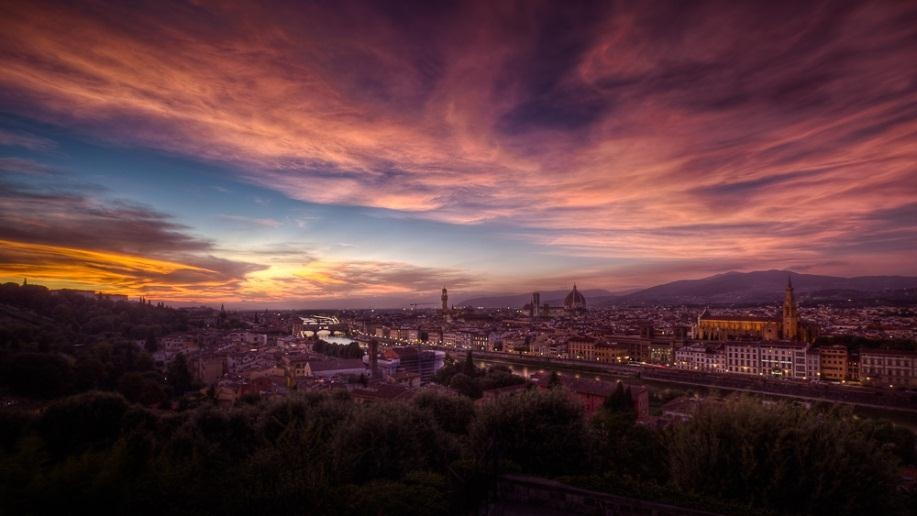
\includegraphics[width=0.2\textwidth]{figures/introduction/examples of applications/1Automated Aesthetic Analysis.pdf4.jpeg}}
    \vspace{3mm}
    \subfloat[Image After Automatic Crop Enhancement\cite{Schifanella2015}]{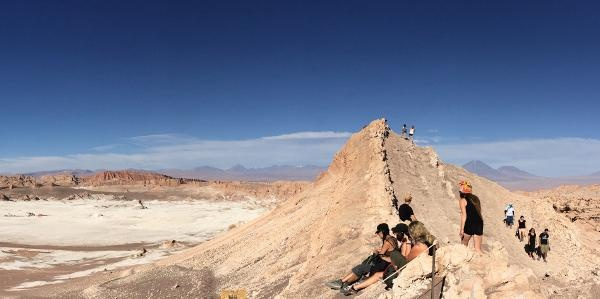
\includegraphics[width=0.2\textwidth]{figures/introduction/examples of applications/7Learning to Compose with Professional Photographs on the Web.pdf6.jpeg}}
    \caption{Image Enhancement Examples From IAQA Literature}
    \label{fig:enhancement}
\end{figure}


Other applications include the selection of product photographs that are most likely to be of higher quality and hence more attractive to consumers, or of the most appealing architectural photographs of hotels. One real-world example of this is Idealo\cite{idealo2021}, who provide a service and commercial applications of IAQA\cite{Talebi2018,Lennan2018}. 

\begin{figure}[ht!]
    \centering
    \hfill
    \subfloat[On Device Rating\cite{Lo2013}]{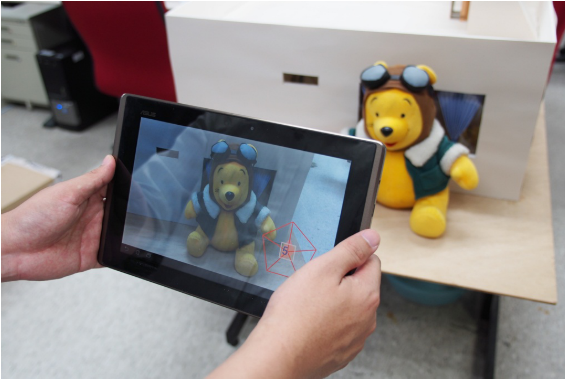
\includegraphics[width=0.2\textwidth]{figures/introduction/examples of applications/on_device.png}}
    \hfill
    \subfloat[Aesthetic Attributes\cite{Lo2013}]{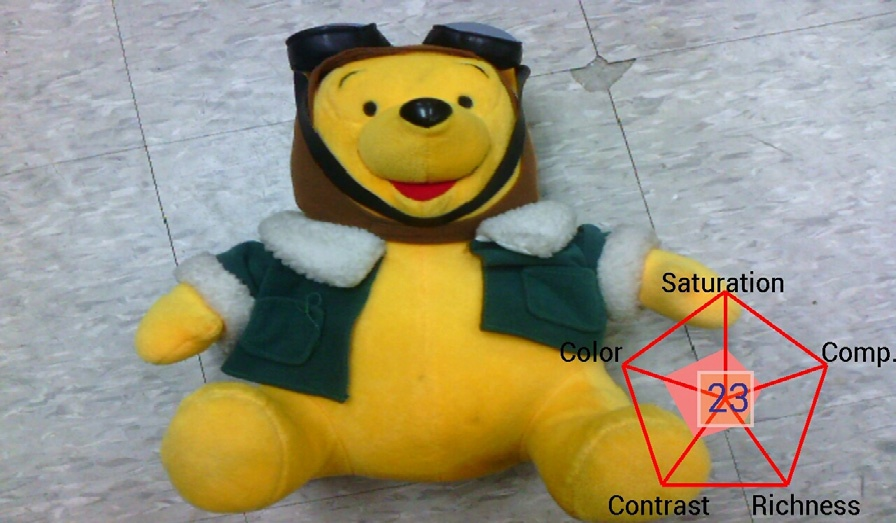
\includegraphics[width=0.2\textwidth]{figures/introduction/examples of applications/10Intelligent Photographing Interface.pdf1.jpeg}}
    \label{fig:on device}
    \hfill
    \subfloat[Predicted Attributes Scores (Radar Maps)\cite{Jin2019}]{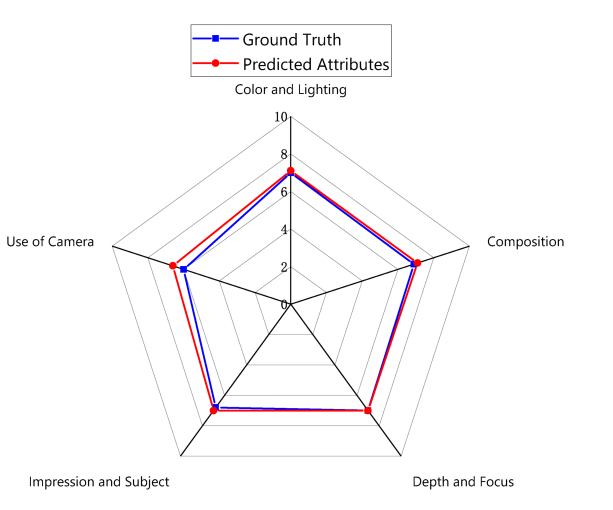
\includegraphics[width=0.2\textwidth]{figures/introduction/examples of applications/atributes_map_jin2019.png}}
    \hfill
    \subfloat[Best Handy Shot\cite{Schwarz2018a}]{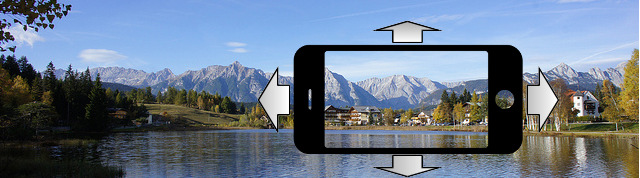
\includegraphics[width=0.2\textwidth]{figures/introduction/examples of applications/wschwarz2018a.png}}
    \caption{Application Examples (On Device Rating, and Best Hand Shot)}
    \label{fig:on device}
\end{figure}

More widely, there are numerous fascinating examples of computer vision in aesthetics - such as pose analysis of ancient art, and art restoration and verification where computer vision is being applied to verify a painting's authenticity\footnote{\href{https://art-recognition.com/}{https://art-recognition.com/}}\cite{Snow2017} and in generating novel images\footnote{\href{https://www.artbreeder.com/}{https://www.artbreeder.com/}} and include computer vision applications of style recognition\cite{Cheng2021} shown in figures (\ref{fig:origional}, \ref{fig:style}, \ref{fig:transfer}).

\begin{figure}[ht!]
    \centering
    \hfill
    \subfloat[Original Image \cite{Cheng2021}]{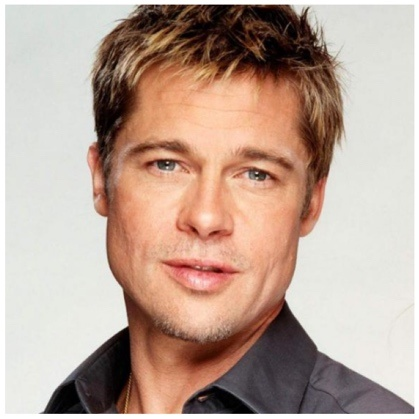
\includegraphics[width=0.2\textwidth]{figures/introduction/style_transfer_brad_pit.jpeg} \label{fig:origional}}
    \hfill
    \subfloat[Style \cite{Cheng2021}]{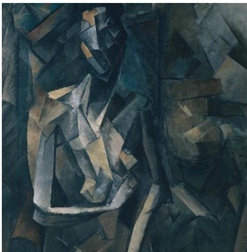
\includegraphics[width=0.2\textwidth]{figures/introduction/Syle Transfer painting.jpeg}\label{fig:style}}
    \hfill
    \subfloat[Style Transfer Image \cite{Cheng2021}]{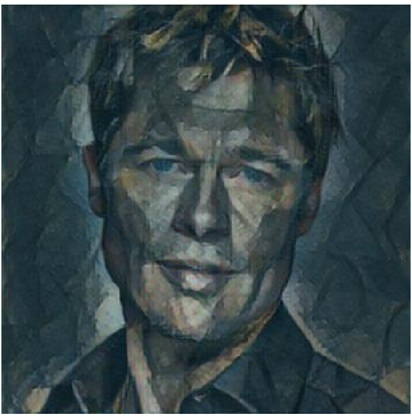
\includegraphics[width=0.2\textwidth]{figures/introduction/Arbitrary_Style_Transfer.jpeg}\label{fig:transfer}}
    \label{fig:style transfer}
    \caption{Examples of Style Transfer}
    
\end{figure}


\newpage


\section{Aesthetics: A Computer Vision Problem}

Computer vision has focused applications stenography \cite{Das2021}, texture analysis,semantic segmentation\cite{Shelhamer2017}, 3D scene reconstruction\cite{Murez2020}, super-resolution\cite{Liang2021} and edge detection\cite{Poma2021} as well as more widely in areas such as object recognition, image captioning, medical imaging. Prior to deep learning  approaches, many techniques involved extracting features using Discreet Wavelet Transoms (DWT)\cite{Makbol2013, Goel2019, Kanwal2021, Goel2014} and  handcrafted or combinations of low and high level feature extraction, where support vector machines (SVMs) are used to enhance for multi-class or object recognition\cite{Makili2011,Goos2016}. 

\par While many of these methods continue to be researched, more recent approaches use Deep Learning - such as attention based salience\cite{Zhu2020}, object detection\cite {Mutch2006, Lei2019, Peng2018}, classification \cite{Jia2020}, and multi-class or active learning\cite{Wu2020a, Joshi2010, Li2004, Gu2015}.

Aesthetics as computer vision problem is further addressed in the Methodology Chapter \ref{chap:Methodology}, and approaches outlined in the Literature Review \ref{chap:Literature_Review} might be considered to be at the intersection of empirical study in the aesthetics of digital photographs (DP), Image Processing (IP), and machine learning (ML). 

\par DP are quantized $\mathbb{R}2$ discrete time images of continuous signal data $\{a,b\} \implies \{x\in \mathbb{Z} : a \leq x \leq b\}$ where $a = 0.4\times{10^{- 4}}$ and $ b = 0.7\times {10^{- 6}}$ frequencies of the electromagnetic spectrum in continuous time in $\mathbb{R}3$ space. IP is a set of techniques used in processing digital images; Machine Learning is a wider umbrella term encompassing approaches such as Deep Learning and Reinforcement Learning (RL). Approaches to deep learning include Convolutional Neural Networks (CNNs)\cite{LeCun1989}, Generative Adversarial Network (GANs)\cite{Goodfellow2020}, Long-Short Term Memory (LSTM)\cite{Hochreiter1997a} and most recently Vision Transformers (ViTs)\cite{Yuan2021, Dosovitskiy2020}. Each field $\in \{DP, IP, ML\} $ (an illustration of this is shown by the Venn diagram in figure \ref{fig:IAQAVenn}) in turn might have further subsets, such as deep learned features as a supervised learning task on a particular subset of DP images, where one type of IP is used for as part of data augmentation. \cite{morris2004computer}.

Many of the traditional approaches to aesthetics have relied on the extraction of hand-crafted features, and are what art criticism would define as formalist aesthetics; texts on formal  photography such as \cite{Kodak1995take}, are frequently cited in computer vision research\cite{Mitarai2013, Murray2012,Talebi2018}. 

\par One clear and obvious drawback of hand-crafted feature extraction approaches, in light of findings across subdomains of aesthetics (empirical aesthetics, philosophy and art), which has been noted in many of the computer science publications\cite{Zhang2021d,Ke2006,Kolesnikov2020,Lu2015b,Birkhoff1933a,Brielmann2018,DaSilva2017,Skov2019} is the not unambiguous in definition(s) of attributes in compounded further by the potential for ambiguity within GT data. Further, although hand-crafted features have produced models that have been able to generalise, they have often been weak learners. Irrespective of recent gains made in computer vision using deep learning, which has come to dominate\cite{Zhang2021d}, it might be argued that these later approaches are better suited to this type of domain - as features are learned, and therefore do not rely on human defined categories but rather on how features that best predict ground truth (GT) labels. 



\subsection{Image Aesthetic Quality Assessment IAQA}

One conceptual challenge in defining a domain within aesthetics or vision is the question of whether aesthetic appreciation is cognitive, a property of stimulus itself, or something that can be objectively assessed as a quantitative and computational task. 

\par This ambiguity has been highlighted even in early canonical attempts at analysis of aesthetics; Kant in 1892, for instance, introduces in his critique of judgement the notion simultaneously that 'beauty is in the eye of the beholder'\cite{Zhang2019} while judging something as good - is to 'to make [...] a subjective assessment [of what] he has reason for expecting a similar delight from everyone'\cite{Kant1892kant}. The tension between these two statements being an attribute of 'aesthetic' experience\cite{Spratt2015}.
\par
Notwithstanding these inherent ambiguities which are nontrivial, IAQA \textit{has} been extensively researched and formulated as a computer vision problem. Addressing the question of where IQAQ `sits', however, is important in dealing conceptual ambiguity. The importance of clarifying IAQA is fourfold:
\begin{description}
\item[Enables]formulating a problem by understanding of what tools are appropriately leveraged from machine learning and pattern recognition;
\item[Disambiguates] IAQA within nomenclature and sub/super domains where there there is potential for cross over and conceptual confusion; 
\item[Identification] of opportunities for real world application, learning for other domains and clearly;
\item[Understanding] overall purpose and value. 
\end{description}

\newpage

\subsubsection{IAQA definition}

Here the term IAQA is used to disambiguate the field of enquiry, as a term most frequently used in literary criticism and to disambiguate from from fields such as Image Restoration or IQA.

\begin{wrapfigure}[15]{l}{0.5\textwidth}
\specialrule{0.01em}{0.2em}{0.2em}
     \begin{center}
     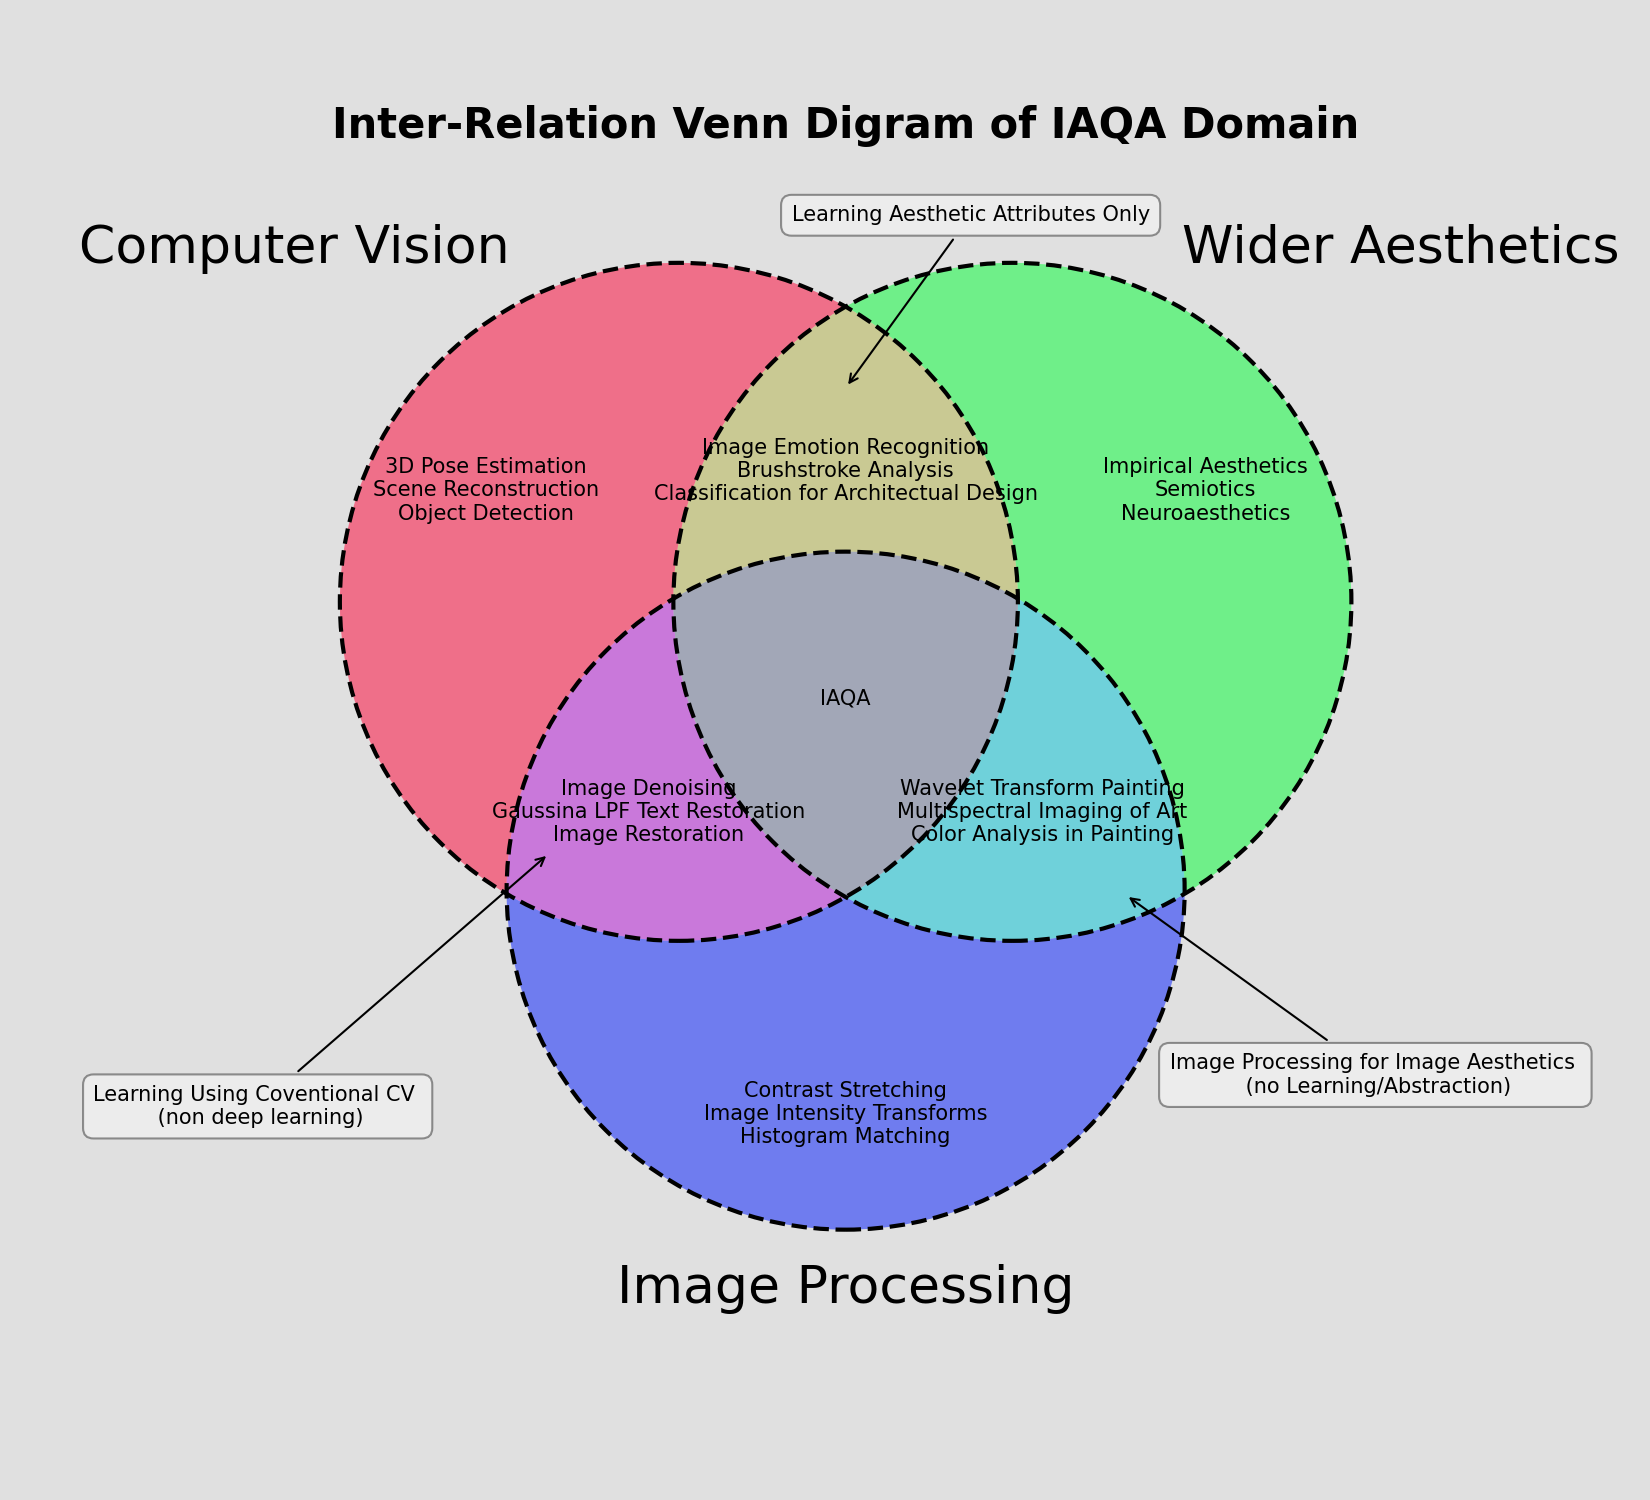
\includegraphics[width=0.45\textwidth]{figures/introduction/inter-relation_of_subjects.png}    
     \caption{Venn diagram Data sets Reviewed in literature reviews }
     \label{fig:IAQAVenn}
  \specialrule{0.01em}{0.2em}{0.2em}
  \end{center}
 \end{wrapfigure}
\par Both Image Processing and Computer Vision are included as separate fields, as there are applications for each within the wider domain of aesthetics - for example, Wavelet Entropy for painting crack identification does not necessarily constitute learning. Here, therefore, it is considered a qualifying feature if IAQA is an application of both Image Processing and Computer vision in the domain of aesthetics\cite{Constatantin2020}. 
\subsubsection{Attention Mechanisms}\\
\par
Within the domain of IAQA, there remains a significant gap between hand-crafted or deep learning models in predicting how a population of human assessors would rate  an image. Further, it is notable that the largest recent gains in predictive accuracy and ability to generalise have come from models that combine deep learning with attention mechanisms. 

\par Attention maps, for example, have been framed as optimisation models to boost a model's ability to learn, to use semantic information, identify areas of focus, or using models trained on salient object detection to inform attention patch centroids.

\subsection{Challenges for IAQA:}

Some of the technical challenges that have been demonstrated to hinder a model's ability to learn are also useful areas for domains more widely. For example image composition is a feature which is challenging to learn where input images and corresponding feature maps of a convolution neural network are necessarily square. These are inherent and no trivial examples of how a CNN might handle real world data, which is potentially messy, ambiguous, and degraded or noisy signal data.


GT is often created by a community of human participants, some of whom may be hobby photographers and others professional. It is unclear whether these rules have been rigorously followed in all cases. Further, in classification tasks or object recognition salience detection, the levels of semantic granularity applied is not so well-defined for IAQA. 

One area of complexity is the clear interplay between context and what is an aesthetic attribute of an image - for instance, a medical image may be considered aesthetically beautiful, or indeed an image from the Oxford flower dataset, and if entered into a competition may score highly. 

\par This may be, for instance, due to the subject matter having a high degree of visual interest that subjectively piques the interest of a viewer with attributes such as visual symmetry. It is clear that both image symmetry and symmetry of a salient object \textit{itself} provide both potential attributes that can be considered aesthetically high value.

\subsection{Challenges/Problem Definition}

Advances in AI in the last decade have seen super-human performance in areas such as deep reinforcement learning and domains with high dimensional search spaces, such as protein folding\cite{Senior2020} and the game of Go\cite{Silver2016}) with its $10^{170} $ possible board combinations. Digital images provide one such example of high dimensional spaces, where an 8-bit  $16 \times 16 $ Red Green Blue (RGB) channel image has $x \in \mathbb{Z} \times 2^{8^{(16 \times 16)}}$ possible pixel combinations.  

Within the wider field of computer vision, the use of deep learning techniques such as convolutional neural networks and transformers in Natural Language Processing (NLP) (and latterly, transformers for computer vision tasks) has resulted in performance accuracy that has increased year on year\cite{Sermanet2014,Simonyan2015a,Szegedy2015, He2016}. 

However, the most recent research papers published on IAQA in 2021 have not achieved accurate scores above 85\% on benchmark datasets. Many of the approaches that have improved CNNs' ability to converge faster and generalise, better such as deeper networks \cite{Simonyan2015a}, adding residual layers\cite{Krizhevsky2017a}, and improving CNN optimisation algorithms\cite{Kingma2015} have seen incremental minor improvements to IAQA.

\par
Significant improvements have generally required attention mechanisms that introduce high-level spatial inductive biases during the training of combined widening or parallel multi-column networks. Many of these represent a replacement of hand-crafted feature extraction, with crafted policies/meta heuristic inductive biases on multi column architectures. 
\par
 With recent metrics for classification CIFAR10\cite{Dosovitskiy2020} >99\% accuracy and CIFAR 100\cite{Foret2020}  96.08\%, image-net 90.88\%\cite{Dai2021}. Notably, \cite{Dai2021,Dosovitskiy2020} are both convolution transformer hybrid (ConViT) models. While \cite{Foret2020} is not a ViT-hybrid, it is only marginally better in performance than its next nearest neighbour \cite{Dosovitskiy2020}. These metrics are so accurate that it would be important to ask if an individual human subject would be able to perform so well. Many of these improvements remain within narrower applications, where CNN's have already achieved high levels of accuracy and have remained dominant\cite{Krizhevsky2017a,LeCun1998,He2016a}. 

ViTs, to our knowledge, have not been used for IAQA, have traditionally required huge datasets\cite{DAscoli2021, Touvron2020a, Khan2021}, and only generalise well on datasets (14M-300M) images\cite{Dosovitskiy2020}.

\par Datasets of this size do not exist for IAQA. Recent approaches using transfer learning are producing data efficient transformers\cite{DAscoli2021}, however it is unclear, when compared with conventional approaches on smaller tasks and on new domains, whether ViTs or ConViT's outperform CNNs. 

Here, we will \textit{compare} and \textit{contrast} the best performing CNNs with ViTs and ConViTs, and evaluate performance within the IAQA domain with binary (high, low) quality images, and attempt to predict how a compute of online voters would score an image. 

\section{Aims and Objectives}

\label{aims and objectives} 

The objective of the dissertation project outlined here is to review IAQA using the AVA benchmarking dataset as a binary classification problem. This will be outlined within the context of wider datasets and implementation challenges, and the training of state of the art models using domain adaptation vision transformers and will outline what makes IAQA important.

Key aims and objectives are:
\begin{enumerate}
    \item \textbf{Aims:} The aims of a this dissertation project are:
        \begin{itemize}
        \item To build an understanding of previous computer vision research in the domain of IAQA;
        \item To compare pre-existing CNN architectures with Vision Transformers (ViTs) and ConViTs;
        \item To further knowledge on what state of the art models can contributions in the domain of IAQA;
        \item To train, adapt and test\emph{existing models} using available code;
        \item To identify areas for future development;
        \item To generate new learning by training models that have not yet been used within IAQA such as Vision Transformers.
        \end{itemize}
    \item \textbf{Objectives:}
        \begin{itemize}
            \item To evaluate different ViT, ConViT and CNN models;
            \item To improve models by adjusting hyper perimeters and selection of appropriate data augmentation;
            \item To address challenges inherent withing the data such as \emph{class imbalance};
            \item To report metrics on architecture performance of base-line and state of the art approaches;
            \item To produce trained models that can be used for inference on unseen data;
            \item To provide provide analysis of models using both quantitative and qualitative results;
            \item To provide analysis and rational for the selection of models;
            \item To report results reproduced in by existing research withing the domain of IAQA. 
        \end{itemize}
\end{enumerate}

\section{Contributions}

The contributions made here are chiefly of a novel approach to IAQA using ViTs and ConViTs (the first application of ViTs and ConViTs) to the field of IAQA. We demonstrate this contribution by:\begin{enumerate}
\item Comparing side by side with CNNs;
\item Show both quantitative and qualitative results of inference;
\item Conducting analyse of how both transfer learning can be used with minimal additional training.
\end{enumerate}

Within literature review we conduct a review of datasets on IAQA and conduct analysis of dataset sizes and type and produce a proposed data dictionary which would be us full for further IAQA research, we also aggregate dataset size and type which is currently missing from IAQA literature and hope that this will be useful for further research within IAQA. 

We also web scrape and produce a data dictionary of all 320k images available on dpchallenge.com which would facilitate further research including multimodal research an make use of the rich comments data that is available on dp.challange.com.

We also conduct analyse of Ava Benchmark Dataset and show that their is a statistically significant relationship between the competition and mean observed score (MOS) where competition number increases monotonically with time. 

\section{Thesis Organisation}

The thesis introduction (chapter \ref{chap:Introduction}) has provided a high-level overview of the IAQA domain and potential applications. It will also introduce the current context, challenges and problems alongside providing context on aesthetics. 

\par The literature review (chapter \ref{chap:Literature_Review}) will provide context on both datasets and provide insights into how different publications have address the challenges of CV in IAQA; further it will review available data an provide justification for using the AVA Benchmark dataset based based on available literature and also outline evaluation metrics used.

\par

Research methodology (chapter \ref{chap:Methodology}) will outline the approach taken to data handling, the image processing pipeline, and to the training of models. Results and discussion (chapter \ref{chap:Results}) will provide both qualitative and qualitative outcomes of the various CNNs and ViTs that were trained. 

\par Chapter \ref{chap:Conclusion} provides future recommendations and outlines major contributions and the significance of the findings.

\newpage

\begin{enumerate}
 \item \textbf{Key Aspects:} within \ref{chap:Introduction} \emph{Introduction}.
        \begin{itemize}
            \item Introduce the application domain of IAQA \emph{aesthetics};
            \item Provide an initial outline of the problem and state of the art metrics(SoTA) on image classification;
            \item provide a \emph(lens) through which to read the following chapters. 
        \end{itemize}
 \item \textbf{Key Aspects:} within \ref{chap:Literature_Review} \emph{Literature Review}.
        \begin{itemize}
            \item A comprehensive overview of IAQA literature and analysis on different approaches taken;
            \item Evaluation of what was successful and what any drawbacks and pitfalls were within the approaches taken so far;
            \item Provide insights into how findings here can contribute to learning beyond simply attempting to supersede state of the art accuracy on the AVA benchmarking dataset. 
        \end{itemize}
    \item \textbf{Key Aspects:} within \ref{chap:Methodology} \emph{Research Methodology}.
        \begin{itemize}
        \item Vision Transformers overview and adaptation and outline models used and under what settings;
        \item Address challenges posed by the data itself such as class imbalance;
        \item Improve model performance using novel data augmentation techniques;
        \end{itemize}
    \item \textbf{Key Aspects:} within \ref{chap:Results} \emph{Results and Discussion}.
        \begin{itemize}
            \item Evaluate wider significance of research approaches including consideration of cognition and where IAQA might contribute to wider understanding within the field of computer vision;
            \item Evaluation of what was successful and what any drawbacks and pitfalls where within the approaches to IAQA thus far taken;
            \item Provide analysis and rational for selection of models used.
        \end{itemize}
     \item \textbf{Key Aspects:} within \ref{chap:Conclusion} \emph{Conclusion} .
        \begin{itemize}
            \item Explore potential future research opportunities;
            \item Outline contribution how this dissertation has contributed to existing knowledge;
            \item Identify potential novel applications, significance and importance of IAQA and computer vision research. 
        \end{itemize}
    
\end{enumerate}

The problem statement of binary classification on the AVA benchmarking dataset is outlined in the introduction and referenced, built on, and evaluated throughout the dissertation. 



% standard chapter format

    
%%%%%%%%%%%%%%%%%%%%%%%%%%%%%%%%%%%%
\chapter{Literature Review} 
\label{chap:Literature_Review}
This section covers the baseline (section \ref{sec:handcrafted}) and state of the art models (section \ref{SoTA})  used within IAQA literature makes a definition of the data used and reviews various Hand-Crafted (HC) as well as deep learning approaches to IAQA. Within deep learning we also include (Vision Transformers) ViTs and (Convolutional Vision Transformers) ConVits  and examine different attention mechanism used in DNNs (section \ref{sec:attention machanisms}). In (section \ref{sec:a case for dl})  we make a case for deep learning over HC feature extraction and the reason for using the Aesthetic Visual Analysis (AVA) benchmarking dataset. We do this through conducting systematic review of datasets and conducting meta analysis of literature through the \textit{`lense'} of datasets used in IAQA literature and descriptive as well as parametric analysis of the AVA dataset meta data (section \ref{sec:related_data}). Finally we outline the evaluation metrics used for IAQA as a binary classification problem in section \ref{sec:evaluation_metrics}. 


%%%%%%%%%%%%%%%%%%%%%%%%%%%%%%%%%%%%
\section{Related Work (Image Aesthetic Quality Assessment)}
\label{related_work}


Image Aesthetic Quality Assessment (IAQA)\footnote{Within the literature on image quality, some publications - which are clearly within the domain of IAQA - refer to this simply as Quality Assessment (QA)\cite{Chang2017}; others heavily blur these categories\cite{Kanwal2021}. For disambiguation, here it is referred to as IAQA so as to delineate the field from other domains - such as image restoration - clearly.} is a highly nuanced and challenging area, which requires care and consideration at several layers of detail. 

\par At a high level within the literature on IAQA, there has been a shift from HC to deep features, in addition to the consideration of either visual attention mechanisms or model architectures. This is reflective of the wider trend in computer vision. Further to what is outlined in the introduction, here we narrow the focus to intra-IAQA literature, rather than interrelated sub-fields or domains that focus on painting or calligraphy\cite{Fernando2021,Sun2015} etc.

There are, to date, four reviews (experimental and literature) on IAQA\cite{Yang2019, Kanwal2021, Deng2017,Spathis2016}. These provide an initial high-level view into IAQA, and cover approaches both HC and many - but not all - of the datasets used in IAQA research publications. The prevalence of citation and review of various IAQA datasets is shown in the Venn diagram (figure \ref{fig:venn}). 


\subsection{Baseline}
\label{sec:baseline}

Initial approaches taken to HC features Trainee Classifier on Support Vector Machines (SVM) or Gaussian Mixture Models: Here, we consider approaches that have used deep learning, alongside performance within IAQA rather than classification more widely.

Deep learning models have generally been binary classification, where MOS is thresholded $<5=0$ and $>5=1$ to produce binary ground truth  of $\in \{0,1\} = \in \{bad,good\}$ image quality. 

As has already been outlined, some form of attention mechanism, paralleling, or patching has been used to improve results on various vanilla CNNs that have been used for IAQA as an image classification problem:\begin{description}
    \item[Alexnet]\cite{Krizhevsky2017a} by \cite{Koa2016b};
    \item[VGG16]\cite{Simonyan2015a} by \cite{Ma2017,Deng2017, Mai2016, Hosu2019, Sheng2018,Ma2017,Kong2016,Liu2017,Koa2016b};
    \item[Inception Nets]\cite{Szegedy2016} by \cite{Liu2020a,Talebi2018};
    \item[GoogleNet]\cite{Szegedy2015} by \cite{Jin2019,Hii2017a};
    \item[DenseNet]\cite{Huang2017} by \cite{Liu2020,Liu2020a};
    \item [MobileNet]\cite{Howard2017} by \cite{Talebi2018};
    \item [ResNets]\cite{He2016a} $\in \{18,34,50,101,152\}$ by  \cite{Sheng2018,Kong2016,Koa2016b,She_2021_CVPR,Chen2020b,Liu2020a}. 
\end{description}  

These report an overall accuracy of VGG with AVA zero padded to square of 72.9\%\cite{Ma2017}, which is significantly less than the performance of ResNet152, reproduced here at 74.1\%. Further, when comparing hybrid vision transformers \textit{ConViTs}, many publications take ResNet architecture as baseline\cite{Wu2021,El-Nouby2021a,Khan2021}, with more recent publications using ResNet152\cite{Jin2019}. Here, training ResNet $\in \{18,50,152\}$ to produce baseline metrics. 

Figure \ref{fig:resnet_block} shows one residual block, of which 18 make up the smaller ResNet figure \ref{fig:resnet_compared}. These networks perform well, and are arguably more competitively efficient with fewer floating point operations (FLOPS). Each block has two weight layers, allowing for an $x$ or identity layer to be concatenated back (a technique for countering vanishing gradients/keeping residual values). All of these networks are trained as baselines without attention mechanisms, but do not require consideration as far as feature hierarchy as this is a built in feature of CNNs\cite{He2016} . Generally within IAQA, where an architecture is used to provide baseline metric, it is also used within a model as a backbone - although, this is not always the case. Authors have taken various approaches to copping, such as canter copping or warping to dimension $ 3 \times 224 \times 224$.  

\begin{equation}
    y = f(x\{W_i\})+x
\end{equation}

Where the output of one residual block x is input $W_i$ are weights of $i_th$ layer in the residual block. 

\begin{figure}
    \centering
    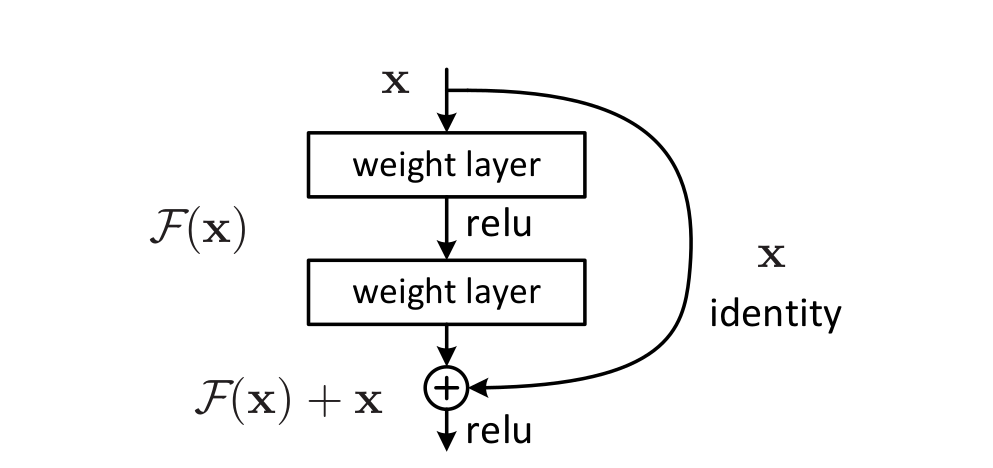
\includegraphics[width=0.38\textwidth]{figures/Literature Review/resnetblock.png}
    \caption{ResNet Block \cite{He2016}}
    \label{fig:resnet_block}
\end{figure}

\begin{figure}
    \centering
    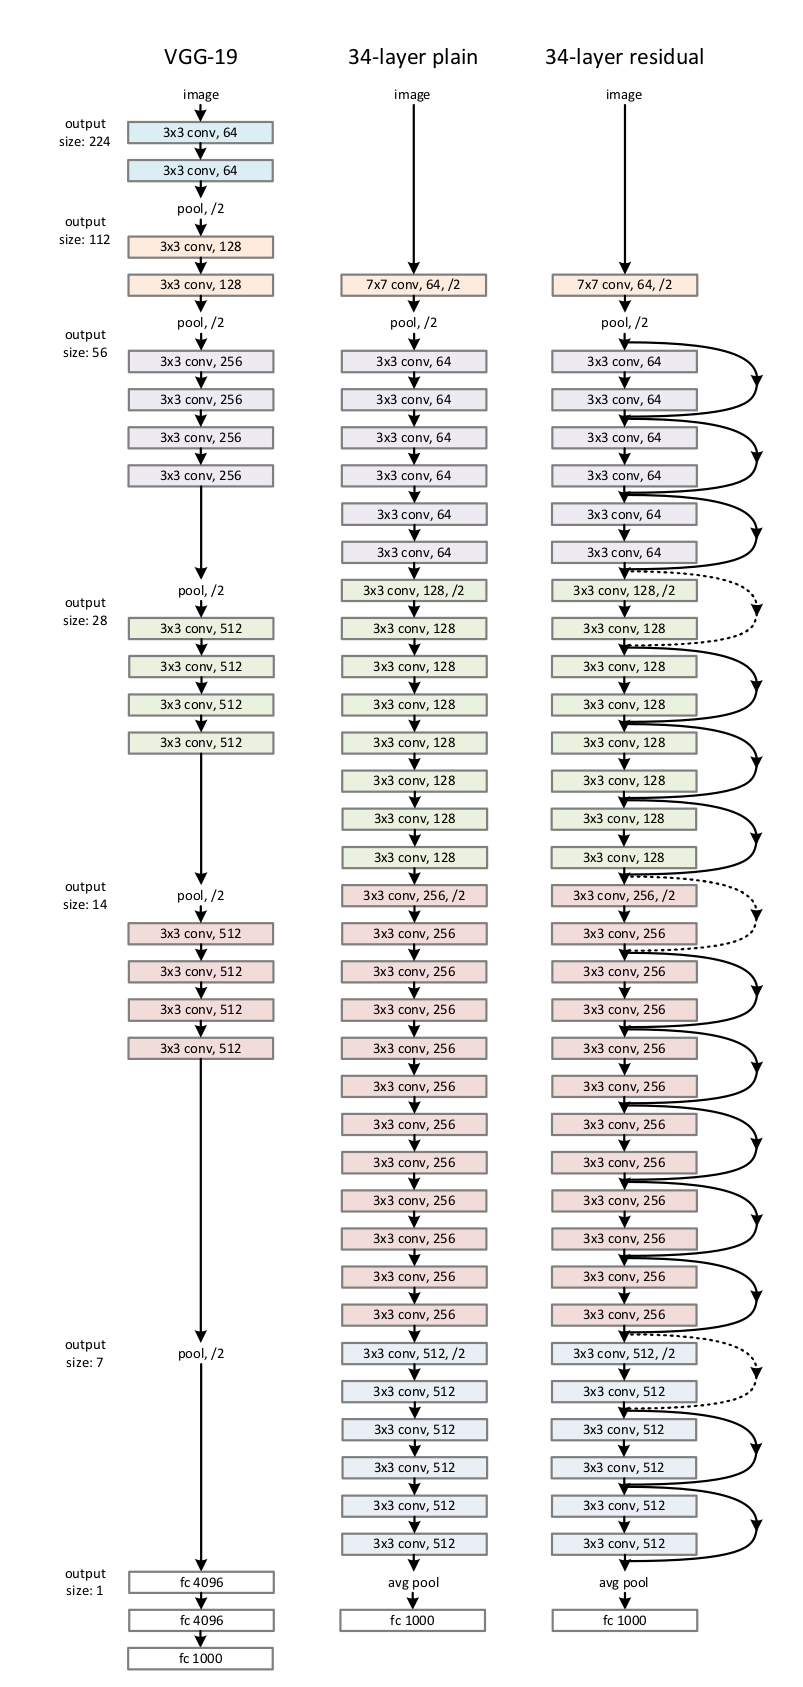
\includegraphics[width=0.3\textwidth]{figures/Literature Review/resnet.png}
    \caption{VGG-19 left , 34 Layer plain middle, ResNet 18 (19 blocks) right  \cite{He2016a}  }
    \label{fig:resnet_compared}
\end{figure}
%%%produced with resent 152,18' 

\subsection{Digital Images}


All of the IAQA techniques reviewed are, by necessity, digital images produced using the sensor arrays of commercially available digital cameras (whose sensors are sensitive to light within an extremely narrow section of the electromagnetic spectrum of $0.4 \times 10^{-4} $ (violet) and $0.7 \times 10^{-6}$ (red)) and digital images discrete quantized representations 0-255 or $0 < (2^{8})-1$ of this spectrum. 

Colour digital images are captured as three channels in an \textit{RGB} image; traditional technique applies functions across an image array $f(x,y)$ where $x$ and $y$ are spatial coordinates of a pixel array. 

\subsection{State of the Art (SoTA)}
\label{SoTA}

Three main and closely interrelated features exist for deep learning based models, \textit{multi column}, \textit{patching of image}, and \textit{attention}. For clarity and focus, here we evaluate models that are compared on the AVA benchmark dataset, as it has become the convention within IAQA to benchmark on AVA dataset. 


\subsubsection{Multi Column} 

 Almost all models have used some form of multi column image classification network as a backbone; the performance accuracy of each is shown in \ref{tab:SOA}. 
 
 Even where the multi patch is not apparent in name, this is embedded in the approach in some way. Early models, such as rapid \cite{Lu2014a}, almost replicate the extraction features and constitute HC thinking, but as a \textit{policy} for a paralleled CNN, where the focus has been to train to classify based only on 'textures' (and then implement a voting system\cite{Lu2014a, Wang2016c}), the most basic of these simply bolt on an SVM classifier to label parts of the dataset $\in \{scene, object, texture\}$ and then pass these to a separate forward feed network. \cite{Koa2016b, Sheng2018} have separated learning tasks where semantic information is learned and use this alongside aesthetic to enhance predictive ability by concatenating weights back using a Bayesian probability graph at the end of the model. 
 
 Others have defined columns that train on spatially local patches that are selected via an attention mechanism, frame patches as an optimisation system, or they create a multi-patch aggregation system \cite{Lu2015b,Sheng2018}. The most complex of these are similar to policies\cite{Sutton2018} within reinforcement learning (RL) and \cite{Sheng2018} learning optimisation algorithm. For instance, this even appears to obey a Markovian property - further underscoring the parallel. However, authors do not themselves make this observation or frame learning in this way - perhaps it would have enriched their work if they had. 

\begin{figure}
    \centering
    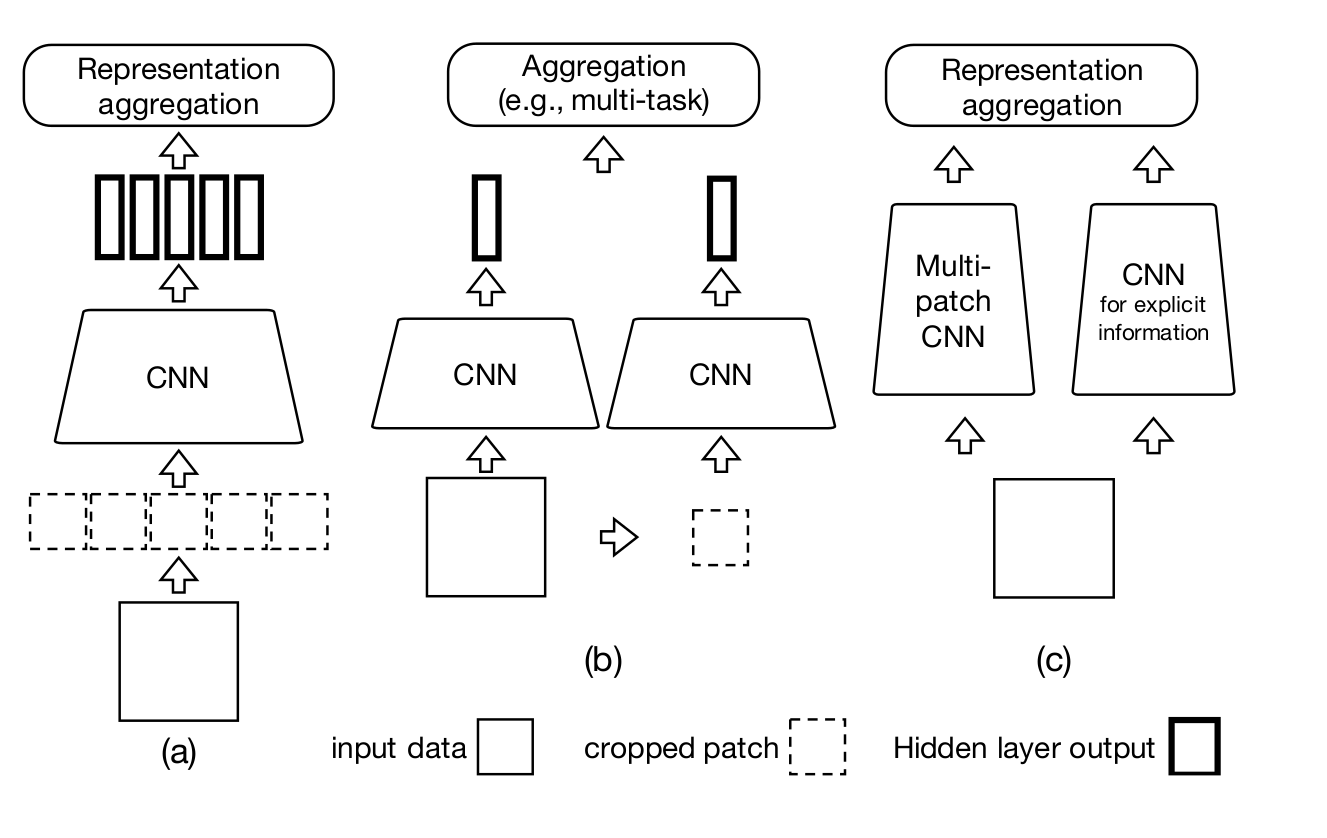
\includegraphics[width=0.3\textwidth]{figures/Literature Review/newtworks/Sheng2018_attention_based_MP.png}
    \caption{Aggregation based architectures for IAQA  \cite{Sheng2018}}
    \label{fig:MPADA}
\end{figure}


\subsubsection{Attention mechanisms} 
\label{sec:attention machanisms}

All of the state of the art models considered here are produced using attention mechanism or multi layer architectures that have been used to successfully improve classification accuracy, and produce models that perform better than vanilla networks on the AVA test set. 

Some of these approaches, such as A-Lamp \cite{Ma2017}, use adaptive patch selection based on the most informative patches, using graph based salience detection, to select multiple patches shown in figure \ref{fig:graph_patch}. 

Various iterations of this have been the rule within recent IAQA literature, and these have been to solve a range of technical challenges, which fall into the categories of \textit{spatial com positional, spatial intentional and semantic}. 

Spatially based attention is developed as a learning policy by \cite{Sheng2018}, who employs an optimisation strategy to maximise training accuracy by selecting new patches and avoiding bounding box coordinates of the previous patch for n attempts. Other attempts have sought to create a policy where a model can focus on aesthetically similar images \cite{Schwarz2018a}. 

Some have cropped salient patches a without any other transforms and built an attribute relation graph \cite{Ma2017}. The most recent and sophisticated of these create and utilise aesthetic related attributes and spatially related regions\cite{She_2021_CVPR} or use multi-modal approaches\cite{Zhang2021d} that leverage comments and information to combine self attention with attention based on LSTM trained on said comments. 

The latter two approaches mark the the most significant improvements in overall accuracy in the AVA bench marking, and represent a leap of significant margin. One drawback of these approaches is that they do not necessarily lend themselves to easy application, and are difficult to validate. Further, each approach somewhat reinvents the wheel in terms of attention mechanisms; none of these approaches have used a vision transformer or hybrid \textit{Convolutional Vision Transformer (CvT)} network.  

\subsubsection{Image Patching}
\label{sec:image patching}
%%%%%%%%%%%%%%%%%%%%%%%%%
% include eg from alamp %
%%%%%%%%%%%%%%%%%%%%%%%%%
The mean image size of the AVA dataset is $629 \times 497$ pixels with a maximum of $800^2$ pixels. The convention in almost all of the approaches sub-sample, down-sample, or crop images as part of data augmentation. This is often the first process in image augmentation; image patches are in most cases $3\times224\times224$, however, in some cases images have been warped to square before patching \cite{She_2021_CVPR} and others have been zero-padded to preserve composition. 


\begin{figure}
    \centering
    \begin{subfigure}[b]{0.25\textwidth}
        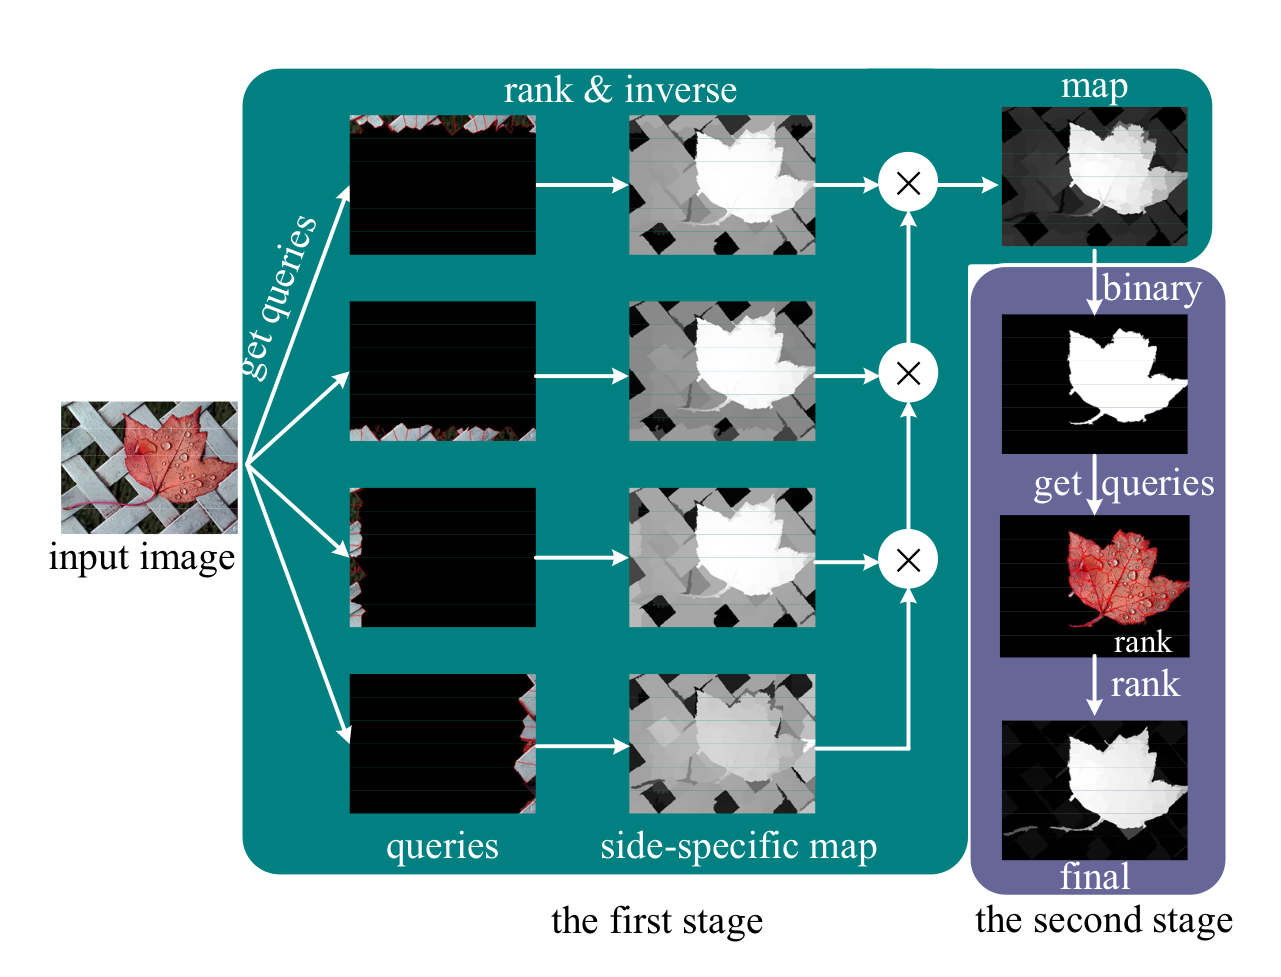
\includegraphics[width=\textwidth]{figures/Literature Review/yang2017_graph_based.png}
        \caption{Patching Example From Hand-Crafted Features \cite{Yang2013}}
        \label{fig:graph_patch}
    \end{subfigure}
    \hspace{5mm}
    \begin{subfigure}[b]{0.3\textwidth}
        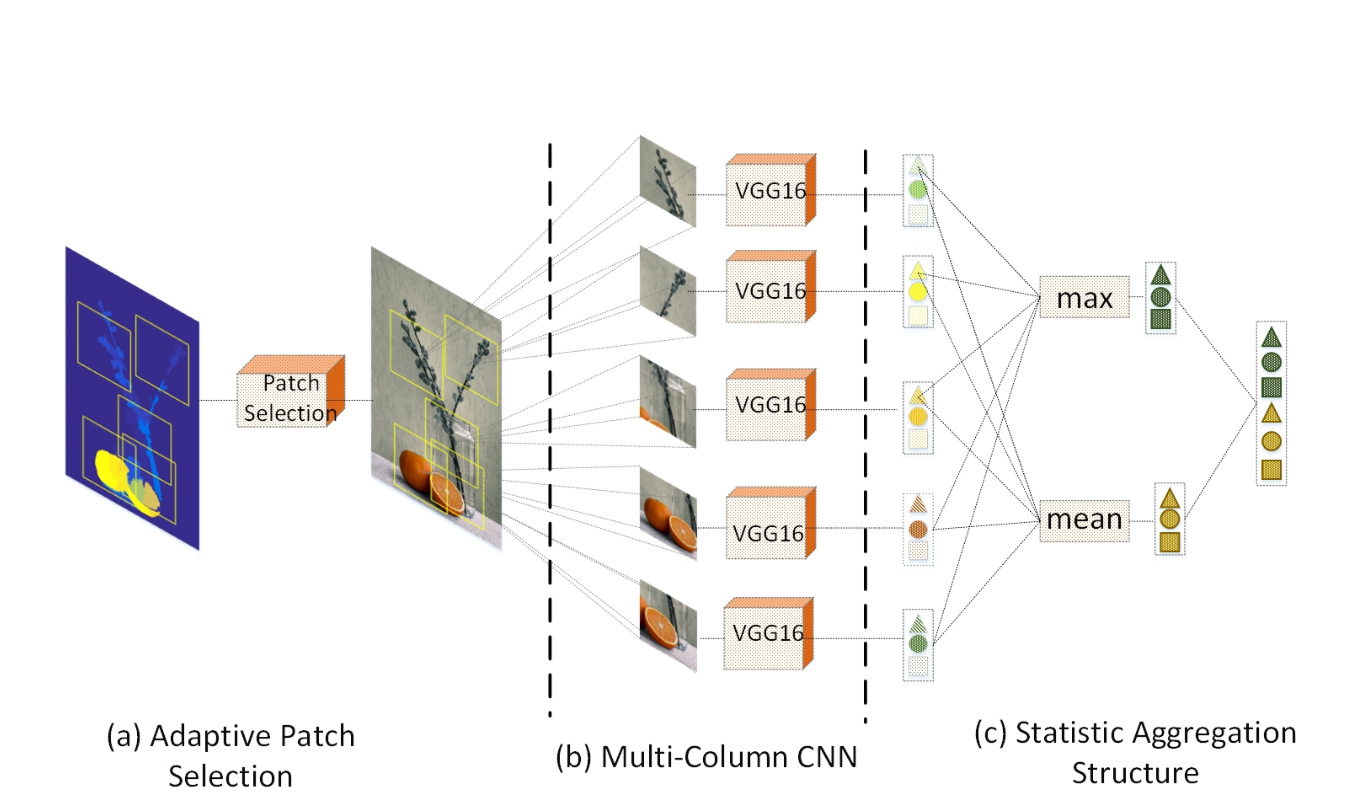
\includegraphics[width=\textwidth]{figures/Literature Review/alamp_patch.png}
        \caption{A-Lamp Multi Patch Network  \cite{Ma2017}}
        \label{fig:alamp_multi}
    \end{subfigure}
    \hspace{5mm}
    \begin{subfigure}[b]{0.25\textwidth}
        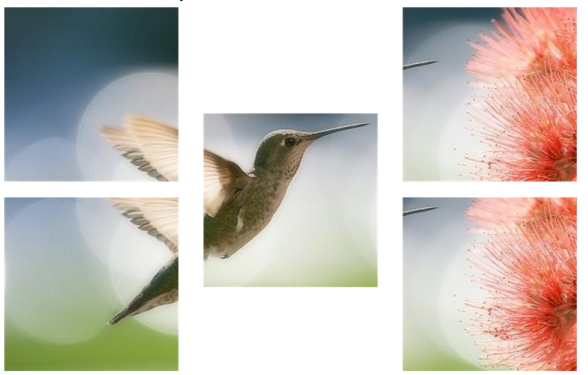
\includegraphics[width=\textwidth]{figures/Literature Review/alamp_bird.png}
        \caption{Patches Taken From AVA Dataset Based on Saliency Graph \cite{Ma2017}}
        \label{fig:alamp_patches}
    \end{subfigure}
    \caption{ Patching Examples from Hand-Crafted \cite{Yan2013} and Deep Features   \cite{Ma2017}}
\end{figure}



\begin{table}[ht]
\tiny
    \centering
    \begin{tabular}{c?p{2cm}ccp{2.5cm}c }
 \specialrule{.1em}{.1em}{.1em}
 \multicolumn{6}{c}{*State of Art Models and Metrics on AVA Dataset*}\\
 \specialrule{.1em}{.1em}{.1em} 
  \textbf{Year} $\downarrow$  &  \textbf{Model} & \textbf{Reported Acc.} $\downarrow$ & \textbf{Reproduced Acc.} & \textbf{Approach} & \textbf{Backbone} \\
 \specialrule{.1em}{.2em}{.01em}
  2014 & RAPID DCNN\cite{Lu2014a}& 75.4        & -- & Double column CNN (texture) & AlexNet\\
  \specialrule{0.01em}{0.1em}{0.1em}
  2015 & DMA-Net \cite{Lu2015b} & 75.4 & -- & Multi-column & Alexnet\\
  \specialrule{0.01em}{0.2em}{0.1em}
  2016 & A\&C CNN\cite{Kao2016} & 74.5      & --& Scene Object Texture (multi attr./col.) & Rapid CNN\cite{Lu2014a} \\
  \specialrule{0.01em}{0.2em}{0.1em}

  2016  &  MNA-DCN\cite{Mai2016}    & 77.1     & -- & Adaptive Spatial Pooling  &  VGG-16\\
  \specialrule{0.01em}{0.1em}{0.1em}
  2016 & MNA-CNN-Scene\cite{Mai2016} & 77.4 & --& Multi-Column (spatial)  & VGG16 \\
 \specialrule{0.01em}{0.2em}{0.1em}
  2016 & BDN\cite{Wang2016c}     & 78.9     & --& Multi column (directed augmentation)   & Custom Auto Encoder    \\
  \specialrule{0.01em}{0.2em}{0.1em}
  2016 & MTCNN \cite{Koa2016b} & 79.1 & -- & Baysian Multi Task  & AlexNet, VVG Net, ResNet\\
  \specialrule{0.01em}{0.2em}{0.1em}
  2017  &  New-MP-Net\cite{Ma2017}    & 81.8     & -- & Multi-Patch     & VGG-16\\ 
  \specialrule{0.01em}{0.2em}{0.1em}
  2017 & MultiGap\cite{Hii2017a} & 82.27 & -- & Multi pooled with text augmentation & GoogLeNet\\
  \specialrule{0.01em}{0.2em}{0.1em}
  2017 & A-Lamp\cite{Ma2017} & 82.5        &-- &  Adaptive-Multi patch (spatial)  & VGG16\\
  \specialrule{0.01em}{0.2em}{0.1em}
   2018 &   NIMA \cite{Talebi2018} & 81.51    & 77.36  & Reproduces MOS Distribution & Inception-v2, MobileNet\\
  \specialrule{0.01em}{0.2em}{0.1em}
    2018 &   MPADA\cite{Sheng2018}        & 83.03    & 79.1   & Attention Based Multy-Patch & Resnet18\\
  \specialrule{0.01em}{0.1em}{0.1em}
  2019  &  MLSP\cite{Hosu2019}          & 81.72    & 81.7   & Double column CNN &VGG-16 \\
  \specialrule{0.01em}{0.2em}{0.1em}
    2020 & AFDC\cite{Chen2020b} & 83.2 & -- & Muli-column adaptive mini-patch & ResNet50, VGG16\\
  \specialrule{0.01em}{0.2em}{0.1em}
  2020 & FCN-A-G\cite{Liu2020} & 83.6  & -- & Region Graph Convolution (fully conv.)  & Resnet101 FCN, VGG-16, DenseNet-121\\
  \specialrule{.1em}{.1em}{.5em}
  2020 & PA IAA\cite{Li2020a} & 83.7 & -- & Siamese Multi-column & Densnet121, Inception-V3\\
  \specialrule{0.01em}{0.2em}{0.1em}
  2020 &   MSCAN \cite{Zhang2021d}       & 86.66    & -- & Multi Modal Self colab. attnt. & VGG16   \\
  \specialrule{0.01em}{0.2em}{0.1em}
   2021 & HLA-GCN\cite{She_2021_CVPR} & 84.6 &  -- & Layout-Aware Graph CNN & Resnet-50, Resnet-101\\
  \specialrule{0.01em}{0.2em}{0.1em}
\end{tabular}

    \caption{State of The Art Metrics (overall accuracy)}
    \label{tab:SOA}
\end{table}

\subsection{Hand-Crafted Features Genealogy}
\label{sec:handcrafted} 

The approaches within IAQA fall into two main categories: hand-crafted (HC) and so-called deep features. HC features are extracted at both \textit{lo} and \textit{high} level and are extracted by traditional approaches to digital image processing\cite{gonzalez2008digital}. 

%%%%%%%%%%%%%%%%%%%%%%%%%%%%%%%%%%%%%%%
% SHOULD THIS INCLUDE A LEVEL EXAMPLE %
%%%%%%%%%%%%%%%%%%%%%%%%%%%%%%%%%%%%%%%





\subsection{Feature Extraction}
\begin{table}[ht]
\tiny
    \centering
    \begin{tabular}{c?p{2cm}p{2cm}p{2cm}cccc}
        \specialrule{.1em}{.1em}{.2em} 
        \multicolumn{7}{c}{* Chronology of IAQA Techniques*}\\
        \specialrule{.1em}{.1em}{.2em} 
        Date & Technique & Feature Type & Extracted (imaging process) &  Feature Levels $\ddag$ & Dataset & Metric & Score\\
        \specialrule{.1em}{.1em}{.2em} 
        2004 & Ada-Boost, Real-AdaBoost (SVM, Bayesian) Classifier\cite{Tong2004} & Texture, Shape, Color, Energy & Band Diff. color histogram, color moment, lab coherence, HSV Coherence, DFT Moment,DCT moment, Wavelet, hist $\in \{Sobele, Laplace, Canny\}$, &  H/L & B$\dagger$ & Linear Corr. & 84.7\% \\ 
        
        \specialrule{0.01em}{0.2em}{0.2em}
        2006 & SVM Binary Classification\cite{Datta2006}& Texture, Familiarity, Size, Depth of field & Wavelet Based and 56 subset functions & H/L & P.Net & ACC  & 70.12\% \\ 
        \specialrule{0.01em}{0.2em}{0.2em}
         2006 &Naive Bayes class \cite{Ke2006}& Glob Edge Distribution, Color Dist., Lo-level Contrast, Brightness indicator   & Laplace Filter, KNN, 20bin Histogram, Fourier Transform & H/L& DPC & ACC & 72\% \\
        \specialrule{0.01em}{0.2em}{0.2em}
        2008 & SVM, Gentle ADABoost, Bayes Classifiers\cite{Lou2008} & clarity, contrast, lighting, simplicity, composition geometry, color harmony & Histogram, blurring kernel, $f(Hue \times Bri. \times Sat.)$& H/L & DPC & max AUC &  $93\%$\\
        \specialrule{0.01em}{0.2em}{0.2em} 
         2009  & SVM Classifier\cite{Wong2009}& salient object, subject background  & Saliency Map  & H/L & P.Net &  5CV-ACC & 78.8\\
        \specialrule{0.01em}{0.2em}{0.2em}
        2011&SVM Classifier \cite{Dhar2011}&Colour, DOF, Illumination of sky & Color spatial dist., multi scale contrast, Wavelet Energy, Haar Features, Spatial Pyramid Shape &H/L &DPC/Flkr. & ROC & -- \\
        \specialrule{0.01em}{0.2em}{0.2em}
        2012 & SVM Classifier\cite{Lo2012a} & Layout, Composition, Texture, color& Hist, FFT, kNN(color) & H/L & CUHK &  mean ACC &  86\%\\
        \specialrule{0.01em}{0.2em}{0.2em}
        2013 & SVM Classifier\cite{Tang2013a} (feature prediction) & Geometric composition, Complexity, DOF, Hue Composition, Blur, Brightness & Color harmony $f$, Orientation $f$, Salience map, Kernel Blurring &  H/L & CUHKPQ & max AUC &  $<80\%$\\  
        \specialrule{0.01em}{0.2em}{0.2em}
         2015 & Bayesian Network Support Vector Regression (SVR)\cite{Gao2015a}&17 High level & SSIM, SIFT, HOG &  G & DPC/PNet &ACC & 72.7 &\\
        \specialrule{0.01em}{0.2em}{0.2em}
         2015&SVM  Classifier \cite{Mavridaki2015}&  Proposed
         Simplicity, Colorfulness, Sharpness, Pattern, Composition & Histogram Wavelet coefficients, Euclid distance, Color histogram & H/L& CUHK-PQ/AVA & ACC & 77.1\% \\
        \specialrule{0.01em}{0.2em}{0.2em}
        2016 &SVM \cite{Wu2016}  &  Aesthetic Class & mulitmodal,Structural Features, Local Vision features, Functional purpose& H & DS2 &ACC & 78.42\\
        \specialrule{.1em}{.1em}{.2em}
        \multicolumn{7}{c}{$\ddag$ High(H) Low(L) Features, $\dagger$ Bespoke} \\
        
\end{tabular}
    \caption{Approaches to Feature Extraction}
    \label{tab:IAQA Approaches}
\end{table}

Early approaches to IAQA combined 'low-level' features and processes, such as wavelet transforms, to obtain image texture to 'extract' information, or applied coefficients recursively to obtain edge information, or applied some coefficient across an image to compute blurriness. 

The trend in the use of HC features seems to be from multiple complex and individually defined functions, for example \cite{Datta2006} and \cite{Tong2004}, (early examples) both of whom extract 56 and 15 individual features respectively and later examples \cite{Gao2015a} extract only three but apply a more complex learning algorithm. 

\subsubsection{Global/Local}



Almost all approaches use both global features such as texture, and local features such as salient objects. There is some ambiguity in the literature about what constitutes 'local'. Examples of a low-level features are sub-banding in Wavelet, convolving across images, where there is therefor some spatial locality or granularity to the extracted feature. 

\subsubsection{Pipeline}

Many of the features are highly complex functions that have relied on the knowledge of signal processing and making use of Fourier spectrum transforms\cite{Ke2006}, as well as other are more simple histogram calculations (where pixel values are binned into hues) to calculate color harmony.

Figure\ref{fig:handcrafted} shows a typical HC feature extract-on and SVM training pipeline. 

Many of the HC feature extraction approaches reviewed here grouped various features into categories or types such as composition\cite{Lou2008} or blurriness\cite{Ke2006}. Extraction in the design is that of crafting, using engineering skill and domain knowledge to select the design features that correlate with image quality.  

    \begin{figure}[ht!]
    \centering
    \specialrule{0.01em}{0.2em}{0.2em}
    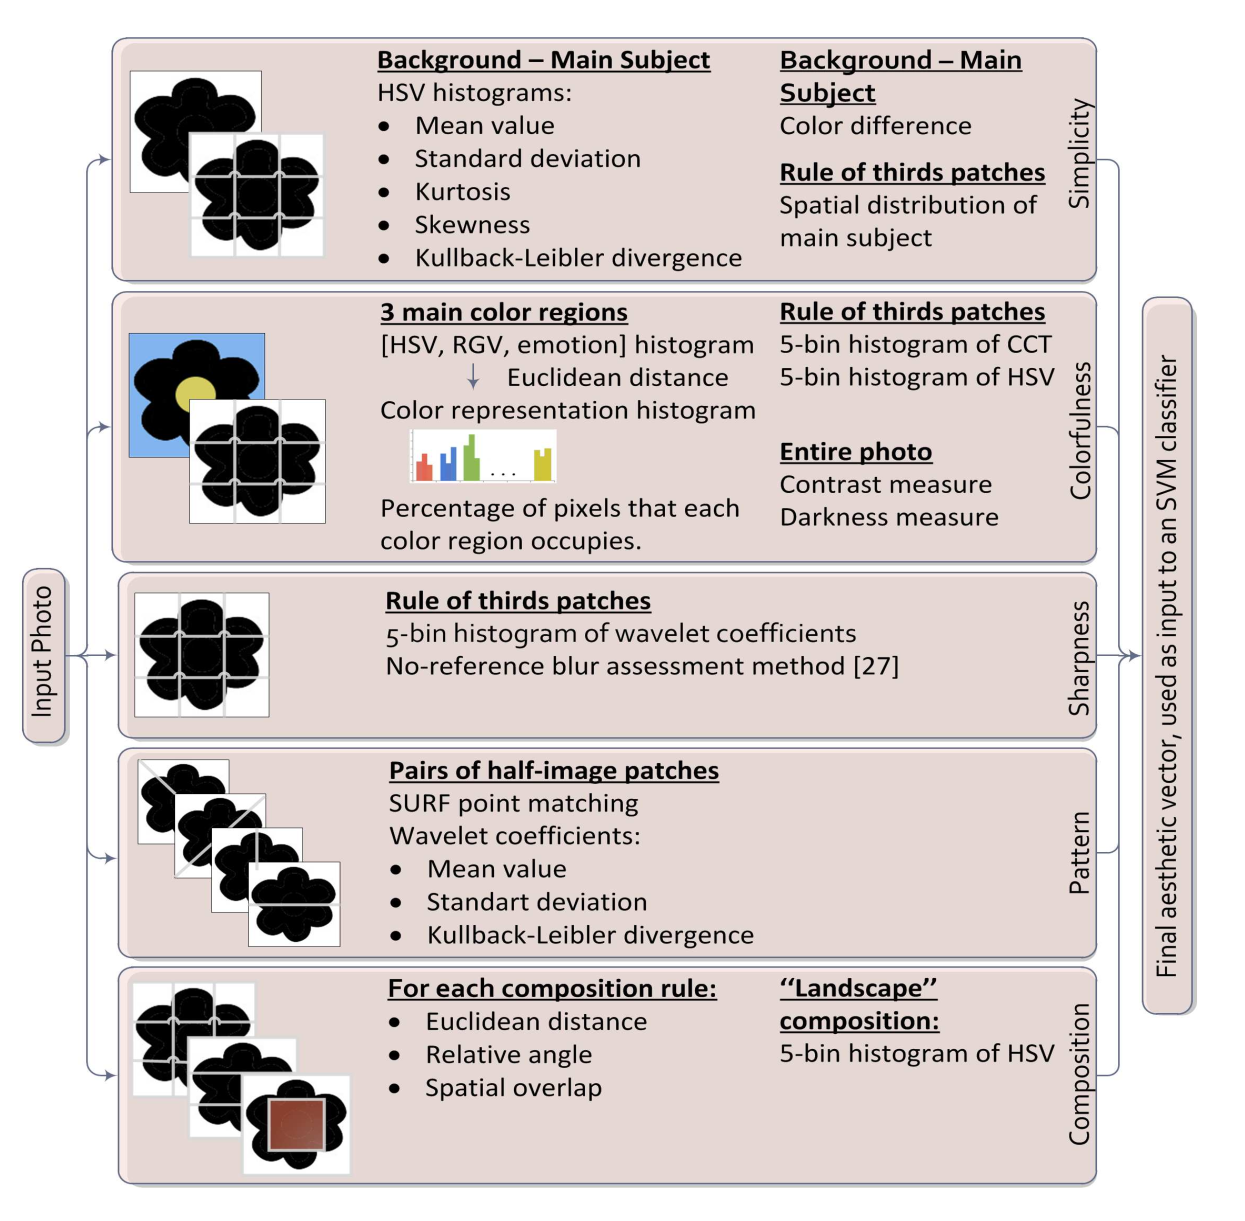
\includegraphics[width=0.5\textwidth]{figures/Literature Review/Hand_crafted/Mavridaki2015_pipline.png}
    \caption{Hand-crafted feature extraction pipeline \cite{Mavridaki2015}}
    \label{fig:handcrafted}
    \specialrule{0.01em}{0.2em}{0.2em}
    \end{figure}

\subsubsection{Convolutionally \emph{or} Conventionally Derived Features}

Approaches, such as convolution operations, which were formerly a mode of implementing a process of applying a predefined coefficient, have shifted to become fundamental and dominant attributes of deep learning for computer vision. 

Deep learning inverts this, making the convolution operator central and neglecting such aspects as high or low-level features, domain expertise, or fundamental understanding of physical properties, which image processing requires. Within this, it is interesting to note that more recent HC feature driven approaches tend to favour simple features and complex image categories\cite{Mavridaki2015,Gao2015a}, perhaps in response to deep learning's dominance? 

Further, of the HC approaches comprehensively reviewed and shown in Table \ref{tab:IAQA Approaches} only one compared results with the AVA dataset \cite{Mavridaki2015} where side-by-side accuracy is 0.77\% on a subset of only top and bottom 10\%(score 1 and score 10) quality images(ignoring 80\%) of data including most ambiguous images. The most accurate binary classification HC approaches were trained on Chinese Hong Kong University-Picture Quality (CUHK-PQ) dataset\cite{Lo2012a}. This dataset is heavily annotated, and has had expert input in rating high and low quality, in addition to being much smaller. All approaches have performed well on this dataset of professional images. 

\subsection{A Case for Deep Learning}
\label{sec:a case for dl}

There is clearly a great deal of interlinking between categories, such as object emphasis, the 'rule of thirds', and shallow DOF, such that a point of focus or object emphasis might be achieved through rule of thirds or shallow depth of field which are categories defined, for example, in the AADB (Aesthetics Attributes Data Base) ( section \ref{iaqa datsets appendix} figure \ref{fig:AADB_1})  with GT labels and HC features. Even 8 HC features can result in a great deal of complexity and ambiguity - not withstanding the high degree of human interpret ability of such concept as a 'balanced element'.

\begin{figure}[ht!]
\specialrule{0.01em}{0.2em}{0.2em}
\centering

\subfloat[${I}\cup{B} \subseteq{O} $]{
  \includegraphics[width=0.2\textwidth]{figures/AADB/feature_venn.png}
  
}
\subfloat[${I}\notin {B} \notin{O} $]{
  \includegraphics[width=0.2\textwidth]{figures/AADB/disjoint.png}
}
\hspace{1mm}
\subfloat[${I}\cup{B} \cup{O} $]{
  \includegraphics[width=0.2\textwidth]{figures/AADB/high_intersection.png}
}
\subfloat[${I}\subseteq{B} \subseteq{}{O} $]{
  \includegraphics[width=0.2\textwidth]{figures/AADB/recursive_intersection.png}
 
}

\caption{\label{fig:AADB_Venn}4 Possible configurations of inter-dependant features within sample space of 8 possible features}
\label{fig:AADB_Venn_}
\specialrule{0.01em}{0.2em}{0.2em}
\end{figure}

This process as has a high-branching factory and  ${\binom{n}{k} = \frac{n!}{k!(n-k)!}}$  possible subsets ${\binom{n}{k}}$ where n is the number of features n and k is number definable or possible features \textit{feature space} that constitute a high quality image. In a search space of $x \in \mathbb{Z} \times 2^{8^{(n \times m)}}$ this is clearly a high number. 

This has the drawback of reliance on human pattern recognition and human defined features, to which machine learning is then applied. In removing the need to define features by hand \textit{a priori}, deep learning represents a paradigm shift and has several advantages for the IAQA domain: 


\par
   
\begin{itemize}

    \item Removal of human bias from feature definition, where definitions within aesthetics remain inherently ambiguous;
    \item Potential ability to generalise better;
    \item Finding patterns in image data that humans would not;
    \item Models can be used to predict image quality of new images easily. 
\end{itemize}

However, while the techniques employed on smaller datasets, such as AADB, may generalise less well on unseen data, HC approaches are appropriate for generating learning from a smaller databases. And approaches that combine both, such as \cite{Kong2016}, provide valuable insights for later analysis. These earlier forays into IAQA should not be disregarded. 
\newpage



\section{Related Data sets}
\label{sec:related_data} 

This section will provide an overview of the different datasets that have been used for IAQA. The purpose of this is to provide further detail, outline some of the inherent challenges, such as class balance within, and how to formulate a problem in such a way as to be able to effectively train and measure against benchmarks, and to illustrate the history and development of the field and draw out how new learning has been generated in previous work.\par

\begin{wrapfigure}[16]{l}{0.5\textwidth}
\specialrule{0.01em}{0.2em}{0.2em}
     \begin{center}
     \includegraphics[width=0.45\textwidth]{figures/data_plots/datasets.png}    
     \caption{\label{fig:Data_venn} Venn diagram Datasets Reviewed in Literature Reviews}
     \label{fig:venn}
  \specialrule{0.01em}{0.2em}{0.2em}
  \end{center}
\end{wrapfigure}
Within the literature that surveys the IAQA domain, there are 15 datatsets (shown in Table \ref{Tab:IAQA Datasets}) that are reviewed in some capacity, and have had publications associated with them. There are also a number of publications that have formed their own bespoke datasets, or which are subsets of existing dataset. In IAQA Reviews \cite{Yang2019,Kanwal2021,Spathis2016,Deng2017}, there are 12 datasets covered. IAQA reviews consistently cover AVA and DPChallenge, however a significant number of datasets are only mentioned by a single source see \ref{fig:venn}, this is reflective of wider IAQA research. \par

Although their are many IAQA datasets,it is clear from the variability both in overall size and type of annotation that, while benchmarking datasets in other areas of computer vision, such as image classification (Cifar $\in\{10, 1000\}$\cite{Krizhevsky2009,Krizhevsky2009a}, ImageNet\cite{Deng2009} $\in \{1K,21K\}$ ), IAQA datasets  are less well defined and readily available. Within this, several subset dataset have been formed to address challenges such a minority class or sparsity of a super set have been compiled. 

\begin{table}[ht!]
\tiny 
    \centering
    \begin{tabular}{c|ccccc}
 \specialrule{.1em}{.2em}{.2em}
 \multicolumn{6}{c}{*Image Aesthetic Quality Assessment Data Sets*} \\
 \specialrule{.1em}{.2em}{.2em} 
 Name &Size \newline (n images) & Classes & Year & Additional & source \\
 \specialrule{.1em}{.2em}{.2em} 
AADB\cite{Kong2016}           & 10,000    & 2           & 2017  & 12 subsets  & Flk.      \\ %have paper
AROD\cite{Schwarz2018a}       & 304,000   & 2  & 2018  &             & Flk.          \\ %have paper \\ 
ALIPR\cite{Datta2008}         & 13,010    & 10          & 2018  & sentiment   & Flk.        \\ %have paper
AVA\cite{Murray2012}          & 255,530   & 10,2        & 2012  & discretized & DPC      \\ %have paper
CUHK-PQ\cite{Tang2013a}       & 17,690    & 2           & 2013  & 7 sub-cats  & DPC          \\ %have paper
DPChallenge\cite{Datta2008}   & 16,509    & 10          & 2008  &             & DPC         \\ %have paper
FCDB\cite{Chen2017}           & 4135      & $\infty$  & 2017  & cropping    & Flk.       \\
Flikr\cite{Yin2012,Chang2017} & 80000     & 2           & 2017  & geo-tagged  & Flk       \\
Flickr AES \cite{Ren2017}     & 40000     & 2           & 2012  &             & Flk.        \\ %have paperh 
IAD\cite{Lu2015a}             & 1,500,000 & 2           & 2014  &             & Multi       \\ %have paper
IDEA\cite{Jin2020}            & 9191      & 10          & 2020  & ballanced   & DPC          \\
PCCD\cite{Chang2017}          & 4135      & 7           & 2017  &             & Bespoke     \\
PD*\cite{Lo2013}  & 1051      & 2           & 2013  &             & CUHK-PK      \\ %have paper
Photo.net\cite{Datta2006}     & 3581      & 7,2         & 2010  &               & P.net   \\ %have paper
Waterloo IAA\cite{Liu2017a}   & 1000      & 7           & 2017  & discretized & P.net          \\ %have paper
 \specialrule{.1em}{.2em}{.2em}
 
\end{tabular}
\caption{IAQA DATASETS}
\label{Tab:IAQA Datasets}
\end{table}

Figure~\ref{fig:Data_venn} shows only three datasets of literature reviewers that are explicitly covered by in all four IAQA review publications( AVA, DPChallenge, and Photo.Net). The AVA Datasets is a super set containing DPChallenge images and is clearly central to the IAQA domain.

IAQA ground truth scores are described through the literature as a distribution MOS (Mean Observed Score). Some datasets have fewer ground truth voters - 28 votes per image photo.net \cite{Murray2012, Wu2011} and others have many raters from a single online community and have 210 per image (AVA); some are rated using a paid for service such as Amazon Mechanical Turk(AMT), or by specialist highly controlled informants where screen and demographic information are recorded in addition to image rating. 
 
 Dataset sizes range from 1100\cite{Liu2017a} Waterloo IAA to 1.4 million\cite{Lu2015a} images (IAD). The mean dataset size overview is 152k images. Figure \ref{fig:IAQA_Data} shows a plot of the dataset against the year of associated publication, and while there does appear to be small positive correlation, there is also an increasing degree of variability in dataset size, with both the smallest and largest datasets being first associated with publications only two years apart.
 \begin{figure}[ht!]
 \hrulefill
 \begin{center}
 \includegraphics[height=0.55\textwidth]{figures/data_plots/iaqa_ds_size.png}
  \caption{\label{fig:IAQA_Data} Dataset Size and Year of Publication Plot}
  \label{fig:IAQA_Data_}
\hrulefill
 \end{center}
\end{figure}
 Further, this divergence seems to increase with time. While available data in other areas of computer vision appears to have increased with time, this is not the case for IAQA, where even very recent publications propose novel datasets such WaterlooIAA\cite{Liu2017}. There is no evidence to reject a null hypothesis that datasets do \textit{not} increase over time.
 
 The MOS distribution of IAQA datasets frequently appears Gaussian\cite{Murray2012, Datta2008, Yang2019, Talebi2018}. AVA is the most normally distributed of these\cite{Murray2012}, where a Gaussian probability density function is given by:

\begin{equation}\label{Gaussian PDF}
f(x) = \frac{1}{\sigma\sqrt{2\pi}} 
  \exp\left( -\frac{1}{2}\left(\frac{x-\mu}{\sigma}\right)^{\!2}\,\right)
\end{equation}



Where $\sigma$ is standard deviation and $\mu$ is mean MOS. The AVA dataset has the most normally distributed dataset of any available IAQA dataset to date\cite{Murray2012}, and has more than 300\cite{AVA2012} associated publications. This is significant in particular for the AVA dataset, where the mean number of votes for each image $ = 210$. This can be taken as a reliable ground truth value, where the probability of an image being scored on some scale is greatest at its mean and enables the exclusion of relatively few images as outliers from a normal distribution. 

Further, it is significant that within this AVA Database of $\approx 255k$ images, only a very small number are excluded as outliers, where an outlier is $\pm4\sigma$, which, while not in itself a test for a normal distribution, shows the normal test for an outlier is $\pm2\sigma$. \par 

This is  consistent with the notion of so called \textit{vox populi} or 'wisdom of crowds' and was initially researched and coined by F. \citeauthor{Galton1907}\cite{Galton1907} in his significant demonstration that mean estimated values of crowds were frequently within $\pm3.1\%$ of ground truth (GT)\footnote{Frances Galton would likely not have used the term ground truth}. 

This significant finding provides a sound reasoning for aggregating crowd sourced scores as a measure of actual image accuracy. One aspect that is not taken into consideration with approximating GT, however, is online community bias, and one point of critique of the AVA dataset is that individual users are not identified and it is further not possible identify how individual users vote over time across different images, or conversely how an online community might vote for different images of the same user.\par 

Classification tasks, which many IQAQ publications employ as routine throughout the literature, compute MOS of each image and then threshold this into usually good or bad image quality categories. This, however, results in class imbalance with the low category as a minority class. The practice of computing MOS (see eq. \ref{mos}) emerged in IQA where HC and traditional computer vision approaches such as\cite{Wang2004} were employed as proxies for GT. 

\begin{figure}[ht!]
\specialrule{0.01em}{0.2em}{0.2em}
\centering
 \includegraphics[width=0.65\textwidth]{figures/data_plots/ava_paramiters_gt.png}
  \caption[width=0.5\textwidth]{\textbf{Left} Compared Gaussian with AVA Distribution of MOS Scores with Gaussian PDF as Defined Above in  \textbf{Right} and Kernel Density of Score: low (0) and high (1)}
  \label{fig:AVA_MOS}
\end{figure}


 Figure \ref{fig:AVA_MOS}, left, overlays plots of gaussian distribution and the AVA dataset (light blue). The line's Probability Density Function (PDF) of a gaussian distribution e.q. \ref{Gaussian PDF} (red) and a computed PDF mapped to AVA MOS scores showing a slight positive skew. The main deviation from this is in values around the mean (note histogram bars above blue PDF). 
 \par 
 
 One potential source of error aggregating human ratings is that it is not possible to rate 0, but it is possible to rate an image at 10. This may account for some psychological bias when rating images . Figure \ref{fig:AVA_MOS} \textbf{right}  appears corroborate this, with the positive scores outnumbering the negative scores and also showing less normalcy of distribution. Figure \ref{fig:AVA_corr} shows that as the number of votes increases, the average score appears to increase with it. 
 
\begin{figure}[ht!]
\centering
\includegraphics[width=0.65\textwidth]{figures/data_plots/MOS_rating_corr_gt.png}
 \caption{ Number of Ratings MOS Correlation \textbf{left} Proportion Positive Correlation with Challenge ID $\Delta T$ \textbf{Right} (With 10 Dimensional Polynomial Fit(Red)}
 \label{fig:AVA_corr}
 \specialrule{0.01em}{0.2em}{0.2em}
\end{figure}

Figure \ref{fig:AVA_corr} \textbf{left} shows both class imbalance (greater high than low) and an apparent increasing proportion of positive score with time. While time is not recorded, with Challenge ID (which increases monotonically) each challenge is opened and closed for a discrete time period. Therefore, it can be shown that there is a positive correlation with change in $\Delta T$ \ref{fig:AVA_corr} \textbf{right} with Spearman's Rank Correlation Coefficient (SRCC) of 0.34 and p value of $3.36 \times 10^{40}$ (this is almost certainly significant).\par 

Accounting for this could take a variety of hypotheses, such as a developing online community within dp.challenge.com. It is certainly clear from reading the comments on dp.challenge.com that there is an apparent social network with many members being persistent - this positive drift could be as a result of cognitive bias? \par 

While some datasets, such as AVA, consist of 250k images (which may have been considered large at its inception), when compared with domains such as object recognition where models can be trained on datasets such as Image-Net (which contains 15 million  images\cite{He2015a}) the available datasets for IAQA remain relatively small. Within the wider field of IAQA, which includes moving images, quality assessment, and fascinating areas such as calligraphy. 

Further, it is important to make a distinction between the field of image quality assessment (IQA) where benchmarking datasets such as LIVE IQA\cite{Ghadiyaram2016} represent images that have been degraded by artificial noise and are used as benchmarks for the sub-field of image restoration within computer vision. 


%%%%%%%%%%%%%%%%%%%%%%%%%%%%%%%%%%%%%%%%%%%%%%%%%%%%%%%%%%%%%%%%%%%%%%%%%%%%%%%%%%%%%%%%%%%%%%%%%%%%%%%%%%%%%%%

%subsection of baseling a

\section{Evaluation Metrics}
\label{sec:evaluation_metrics}

Almost all review approaches to IAQA are binary classification, with few treating as a ten class (reproducing probability distribution of images). 

For classification accuracy, balanced accuracy, and F1 score are reported within the literature; 'accuracy' is the most frequently used metric in IAQA literature\cite{Koa2016b,Schwarz2018a,Lu2014a,Ma2017,Chen2020b,Zhang2021d}. Much less frequent is balanced accuracy\cite{Deng2017} and F1 score by \cite{Ma2017, Mai2016a}. Many approaches use both regression and classification.  

\subsubsection{Accuracy}

'Accuracy' is a measure widely used to evaluate model performance in classification tasks, on both evaluation and test sets. 

\begin{equation}
    Accuracy = \frac{TP+TN}{TP+TN+FP+FN}
\end{equation}

\subsubsection{Balanced Accuracy}

This metric is particularly important in evaluation during the training and testing of models where there is a class imbalance, which is a significant attribute of many IAQA datasets. 

Balanced accuracy in the binary\footnote{for non binary cases, class weights must be computed} case used within IAQA is given by computing the arithmetic mean of sensitivity and specificity False Positive Rate (FPR)(eq.\ref{fpr}) (where sensitivity or true positive rate (TPR) (eq.\ref{tpr}):

\begin{equation}
    Balanced = \dfrac{FPR+TPR}{N_c}
\end{equation}
Where $N_c$ is the number of classes,TPR is given by:
\begin{equation}
    TPR = Sensitivity = \frac{TP}{TP+FN}
    \label{tpr}
\end{equation}
 and FPR is given by: 
\begin{equation}
    FPR = 1 - Specificity = \frac{FP}{TN+FP}
    \label{fpr}
\end{equation}
Other approaches to addressing class imbalance during training and evaluation are discussed below in the Methodology section.


\subsubsection{F1}

F1 score produces the harmonic mean of precision (eq. \ref{precision}) and recall (eq. \ref{recall}) and is given by: 
\begin{equation}
   F1 = \frac{2(Precision \Recall)}{Precision+Recall} = \frac{2(TP)}{2(TP+FP+FN)} 
\end{equation}

where precision is given by:

\begin{equation}
    Precision = \frac{TP}{TP+FP}
\label{precision}
\end{equation}


and recall is given by:

\begin{equation}
Recall = \frac{TP}{TP+FN}
\label{recall} 
\end{equation}

The evaluation metrics outlined here are for binary classification, but a number of approaches train a regression problem first, or compute the mean softmax of ten classes (reproduced score distribution) and use Persons Linear Correlation(PLCC) eq. \ref{PLCC} Coefficient or Spearman's Rank Correlation Coefficient (SRCC) \ref{SRCC}. 

This approach enables distribution analysis also, however it is not always clear in the literature whether a model has been trained purely as a regression model (reproducing MOS). Further, training a ten class problem is less challenging and does not give a good or bad quality estimation. This is particularly apparent with some of the more recent publications that achieve the highest accuracy training models with 10 node output of a fully connected layer. 

In order to be able to produce an end to end network here, we train a binary classifier rather than thresh-holding output computed MOS which approaches such as \cite{Talebi2018,Zhang2021d} appear to take. 


%%%Use your literature review to help the reader to understand the value and the interest in your project.  You should look for related works already published that either support the merit of your project, or provide the background understanding/information to make your new claims.  Try to avoid writing a "catalogue" of related works (e.g this would have little of your own insight added).  Instead, describe to the reader why the related work is interesting or relevant to your own work.  What did they achieve?  What did they overlook?  It is highly recommend you finish your Literature Review with a final subsection "Summary", where you may wish to formulate highly specified research questions or hypotheses, or assert the need for your Research Methodology (next chapter).  

\section{Literature Review Summary}



We show that deep learning has surpassed HC feature extraction on large dataset where IAQA is a binary classification problem and outline why we conduct experiment on the AVA dataset. The role of image processing is now part of data augmentation, however many of the HC approaches provide valuable insights into IAQA features, in part as they require a human understanding of the domain. Deep learning inverts this, making convolution operator central rather than a method of feature extraction, secondly the process of making predictions beyond good or bad is more more straightforward with HC approaches where individual aesthetic attributes can be defined, extracted with a greater degree of explainability. 

While many of the deep learning approaches outperform HC reliant feature extraction, deep learning approaches rely on hand crafting of complex learning policies on equally complex multi column network architectures.


We also show that ther are many IAQA dataset although many are overlapping and subset of larger datasets such as AVA. We also demonstrate that MOS scores approach a gaussian distribution and that there is a large majoriy class.


There is a great deal of literature available on IAQA and specifically using the AVA benchmarking dataset. There also exists some fragmentation within the field with many datasets where it is not always clear whether one is the subset of the other, further dataset metrics are not always reported consistently there are further example of this in the appendix \ref{chap:Appendix}. This is further compounded by a slippage in nomenclature between data source and data set (DP.Challange). This ambiguity exists within publications \cite{Talebi2018} use a 25k test set and \cite{Hosu2019} use the 19k dataset which is from a test train validation split outlined by \cite{Murray2012}. This is further compounded by the fact that the images are different in each subset making side by side comparison challenging. 




%%%%%%%%%%%%%%%%%%%%%%%%%%%%%%%%%%%%
\chapter{Methodology}
\label{chap:Methodology}

To our knowledge, the deep learning networks and architectures adaptations review in \ref{chap:Literature_Review} only include traditional hand-crafted approaches and adaptions of various vanilla backbone architectures. Almost all approaches formulate problems as binary classifications and reproduce overall accuracy. There are two approaches to this: thresh-holded MOS prediction(regression) models output, and training pre-thresholded classes by GT MOS, both with a test train split applied by \cite{Talebi2018,Murray2012}. 

Here, we adopt the latter as a more challenging problem with a clear relationship to real world applications of IAQA and less room for ambiguity within the accuracy metrics (which the authors observe in some of the IAQA literature). 

Some approaches appear to present the accuracy of a ten class (model) MOS, which will give higher accuracy on test data as the trained network will not have to tolerate fully the significant number of images with MOS very close to the high-low class threshold. Further, with a 2 node output vs 10 node there are quite simply 5 times less gradients to vanish. 

Here, we train a various transformer models - both vision transformer ViTs and convolutional vision transformer CvTs. The reasons for this are: \begin{enumerate}
    \item Transformers have not yet been applied to IAQA and a side-by-side comparison generates new insights;
    \item Many deep learning models have relied on hand-crafted attention mechanisms, a process which is a learned intrinsic feature of Vision Transformer(ViT);
    \item Many more recent models have combined deep features with attention layers to obtain the best of both worlds;
    \item There exist a number of pre-trained models on imagined allowing efficient transfer learning to and IAQA Domain.
\end{enumerate}

\subsection{Side By Side Comparisons}
\label{side by side}
Vision transformers require huge datasets and special treatment via custom training schedulers, which have warm-up and cool-down data phases. 

Comparing ViTs, CvTs and CNNs side-by-side on as close as possible training conditions enables an evaluation of whether the introduction of convolution is a means to soften the hard requirements of ViTs during training, providing inductive bias inherent in CNNs. 

We reproduce an example to illustrate how CNNs convolve and maintain spatial proximity. Red shows the kernel and green bounding box shows the image area covered; here, kernel size and stride are parameters that effect feature maps learned. 

\begin{figure}
    \centering
    \begin{subfigure}[b]{0.2\textwidth}
        \includegraphics[width=\textwidth]{figures/research_methadology/mnist_five.png}
        \caption{5 from MNIST Handwriting Dataset \cite{LeCun1998}}
        \label{fig:MNIST 5}
    \end{subfigure}
    \hspace{10mm}
    \begin{subfigure}[b]{0.2\textwidth}
        \includegraphics[height=\textwidth]{figures/research_methadology/mnist_five_convolved.png}
        \caption{\textbf{Convolutions} Filter Kernel of Size (5,5) Stride of (5,1)}
    \end{subfigure}
    \hspace{10mm}
    \begin{subfigure}[b]{0.2\textwidth}
        \includegraphics[height=\textwidth]{figures/research_methadology/mnist_five_patched.png}
        \caption{\textbf{Patches} Filter Kernel of Size (5,5) Stride (5,5)}
    \end{subfigure}
    \caption{Illustration of Spatial Inductive Bias}
    \label{fig:Inductive Bias EG}
\end{figure}

Contrast this with figure \ref{fig:CvT}: patches are exclusive and then attention is learned between \textit{tokenized} discrete patches- clearly a very different paradigm.

We employ domain adaption as an overall approach, where target domain is IAQA binary classification and source domain is multi-class classification convolution architectures of both convolution and ViT models. This brings with it the further strength of being able to use pre-trained models, which do not require compute intensive training from scratch. Transformers require large datasets\cite{Zhang2021,Kolesnikov2020,DAscoli2021,Khan2021,xiao2021early,Wu2021} with then hundreds of millions of labelled data entries\cite{Zhang2021} to converge and produce state of the art metrics, which is much larger than required for CNNs. This is at least in part because CNNs encode prior knowledge (adapting stride and kernal size) of image domain such as \textit{translation equivariance} \cite{Khan2021} across feature maps (figure \ref{fig:Inductive Bias EG} illustrates one example of this), CvTs do not have this as a possible prior embedding; these must be fully learned across discrete patches. Various approaches have been used to improve performance, such as introduction of gated position self-attention (GPSA)\cite{Touvron2021a,Touvron2020a,DAscoli2021}. We will use domain, adaptation, and transfer learning as well as improvements to data requirements that have been introduced. This section will cover our approach on the following areas: \begin{enumerate}
    \item Transformer Architecture
    \item Pipeline and Pre-Procession
    \item{Data Augmentation}
    \item Training Methodology
    \item Testing Methodology
\end{enumerate}



\section{Transformers}
\label{Transformeres} 
Transformers have come to dominate over the recent years in many domains, have outperformed Convolutional Neural Networks (CNN), Recurrent Neural Networks (RNN) such as Long and Short Term Memory (LSTM) architecture\cite{Vaswani2017a} and have become a hot topic. 

Many of these were designed to address challenges such as vanishing gradients, and in many areas, this began with applications such as machine translation within natural language processing (NLP)\cite{Wolf2020a}. These were also areas where attention mechanisms have become an integral part\cite{Vaswani2017a}. 

The transformer consists of blocks (head) in which each learner in sequence learns alignment in K, a value query system where input $Q$is passed to an embedding layer One-Hot tokenization. Input is a tensor of shape $\mathbb{R}^B \times \mathbb{R}^N \times \mathbb{R}^D$ where B is batch size, N is sequence length, and D is dimensional embedding.\cite{Tay2020}. Each attention model architecture can be seen in figure \ref{fig:Vaswani2017a_trans_arch}
\begin{figure}
    \centering
    \begin{subfigure}[b]{0.3\textwidth}
        \includegraphics[width=\textwidth]{figures/research_methadology/tranformer_architecture.png}
        \caption{Attention Model Architecture \cite{Vaswani2017a}}
        \label{fig:Vaswani2017a_trans_arch}
    \end{subfigure}
     \hspace{10mm}
    \begin{subfigure}[b]{0.3\textwidth}
        \includegraphics[height=\textwidth]{figures/research_methadology/multi-head attention.png}
        \caption{Multi Head Attention  \cite{Vaswani2017a}}
        \label{fig:Vaswani2017a_attention}
    \end{subfigure}
    \caption{Initial Attention Model Diagram}
    \label{fig:transformers}
\end{figure}

\subsubsection{Self Attention\label{Attenion_s}}
Attention is is a mapping of query ($Q$), key ($K$), value ($V$) pairing - this is not unlike the python dictionary with a key store. V, K, Q are $MxN$ square matrices. The matrix Q is the product of the computation of a set of queries with all keys\cite{Vaswani2017a} $d_k$ and values $d_v$.  Attention output is given by:

\begin{equation}
    Attention(Q,K,V) = Sotftmax(\dfrac{QK^T}{\sqrt{d_k}})V
\end{equation}

Where $D_k$ is the radical(square root) of the number of patches, a process which avoids vanishing gradients. This attention function is performed in parallel for each head, and these are concatenated back and re-projected. Figure\ref{fig:Vaswani2017a_attention}, the resulting linear output depicted in figure \ref{fig:Vaswani2017a_trans_arch} immediately before softmax layer, which produces class probability. What is learning in this process are linear projections, first local in parallel (each attention head) and then through global projection, produce final values given by:
\begin{equation}
    MultiHead(Q,K,V) = Concat(h_1,...,h_n)W^O
\end{equation}
Where $h_i = QW^Q_i,KW^K_i,VW^V_i$ or the application of attention function to the $i_{th}$ where parameters of multi-head function  are $W_i^Q\in \mathbb{R}^{d_{mdl.}\times d_k},W_i^K \in \mathbb{R}^{d_{mdl.}\times d_k},W_i^V \in \mathbb{R}^{d_{mdl.} \times d_v}, W^O \in \mathbb{R}^{d_{mdl.} \times hd_v}$. Note the last parameter passed is effectively a $O_th$ where $h$ is the number of attention layers\cite{Vaswani2017a}, which is, in effect, a high-level recursive application where power law applies to recursion depth. 

\section{Vision and Convolution Transformers\label{transformer_method}}
\label{ConViTs} 

Here, we initially train Vision Transformers (ViT) - which were adapted as closely as possible from \cite{Vaswani2017a}'s application within NLP by \cite{Dosovitskiy2020} for image classification, a high-level overview can be seen in figure\ref{fig:ViT}. Changes are additional for the final MLP. \cite{Dosovitskiy2020} also shows that attention head can be mapped onto convolutional feature maps. 

Both require flattening of images into 2D exclusive patches $x\in{\mathbb{R}^{H\times W \times C}}$ where $C$ is the number of channels; $H,W$ are the input image height and width; $N$ is patches of image resolution; ($H\times W$) is the resolution dimension of $P^2$ where $W=H$. This is simply $N = \dfrac{W^2}{P^2}$. 

The embedding process that \cite{Dosovitskiy2020} introduces is token embedding $\textbf{E}$  where $\textbf{E}\in\mathbb{R}^{(P^2C)\times D}$  (where $D$ is vector size) and positional embedding $\textbf{E}_{pos}\in\mathbb{R}^{(N+1)}$, which is added to patch embedding to retain position information given by:

\begin{equation}
    Z_O = \begin{bmatrix}
    \textbf{x}_{class};& \textbf{x}^1_p\textbf{E};& \dotsm \ ; & \textbf{x}_p^N\textbf{E} 
    \end{bmatrix} + \textbf{E}_{pos}
\end{equation}

Where $\textbv{E}_{pos}$ is learnable positional embedding shown in dark pink in figure \ref{fig:ViT}, and is added to the concatenated patch embedding(s) back to a final $1\times n$D Vector, hence both global and local self attention can be learned. 

\begin{figure}[h!]
    \centering
    \includegraphics[width=0.8\textwidth]{figures/research_methadology/Dosovitskiy2020_VIT.png}
    \caption{High level overview of Initial Implementation of ViT  \cite{Dosovitskiy2020}}
    \label{fig:ViT}
\end{figure}

\newpage

\subsection{Training Approach}
Transformers require extremely large amounts of data to train, $10 \times$ typically larger than any available IAQA dataset. We combat this in three ways:
\begin{description}
    \item[Transfer Learning] leveraging transformers have been trained on ImageNet1k\cite{Ridnik2021};
    \item[Data-efficiency] using state of the art(SOtA) data efficient transformers\cite{DAscoli2021,Touvron2021a} that are able to train on smaller datasets that have been able to train on subsets of ImageNet1K; 
    \item[Augmentation] using SOtA\cite{Buslaev2020a,Riba2020} approaches such as reflection padding; 
\end{description}
We use pre-trained data efficient transformers developed by \cite{Touvron2020a} models on image net, which introduces soft inductive biases (initialization patches through convolution) developed by \cite{DAscoli2021} and keeping input dimension unchanged at $3 \times 224 \times 224$. Images are resized from the original to the longest edge. In order to preserve computational information, we train on both zero-padded and reflection padded images, where images are grey-scale $224 \times 224$ these are stacked to three equal channels as a simple means to ensure bias is not introduced to the model. We train models of three sizes, of modified data efficient transformer ConViT $\in \{Ti,S,B\}$, which are\cite{DAscoli2021}'s adaptions of DeiT-Ti,DeiT-S,DeiT-B\cite{Touvron2020a}.

\begin{table}[]
    \centering
    
    \begin{tabular}{p{2cm}<{\centering}|p{2cm}<{\centering}c{1.5cm}c{2cm}c{2cm}c{2cm}}
    \specialrule{.1em}{.05em}{.05em} 
         Model & Embedding Dimension & Heads & Layers& Params & Image Resolution   \\
    \specialrule{.1em}{.05em}{.05em} 
    ConViT-Ti & 192 & 3 & 12 & 5M & $224 \times 224$\\
    ConViT-S & 238 & 6 & 12 & 22M & $224 \times 224$\\
    ConViT-B & 768 & 12 & 12 & 86M & $224 \times 224$
    \end{tabular}
    \caption{Efficient ConVits trained adapted from \cite{Touvron2020a,} }
    \label{tab:ConViTs}
\end{table}

The models have a final, fully connected layer of $[1 \times 1000]$ classes, and therefore we add a fully connected layer of $[1 \times 2]$ using PyTorch \lstinline[columns=fixed, language=Python]{nn.Layer(1000,2)} to add a finally fully connected layer to the ConViTs model. We trained ConViT-Ti using a formative grid search, as a new hyper parameter is introduced as a modified Deit-Ti model. This requires significant search, and therefor we only perform a grid search on ConViT-Ti. Trained adjusting hyper parameters incrementally within grid searches for 10 approaches. We also train ConViTs $\in \{Ti,S,B\}$ shown inn Table \ref{tab:ConViTs} with no changes to hyper parameters to provide insights into how including embedded dimension, number of attention heads effects performance on test set. Finally, we train the best model on the best performing hyper parameters. 

\pagebreak  

\subsection{Augmentation} 

%%% transform = transforms_imagenet_train(hflip=hflip,
%                vflip=vflip,
%               color_jitter=color_jitter,
%    
%                std=std,
%                re_prob=re_prob,
%                re_mode=re_mode,
%                re_count=re_count,
%                re_num_splits=re_num_splits,
%                separate=separate)

Data Augmentation is an important part of regularisation in deep learning \cite{Kukacka2017}; it is a powerful way to mitigate against over-fitting during training and supports better generalization\cite{Shorten2019} - ensuring that validation error decreases with training error, we implement conventional methods\cite{Mikolajczyk2018} alongside state of the art methods proposed by\cite{Riba2020,Buslaev2020a}. 

\par

Here, augmentation of images is in two stages: first, all images are square padded to zero to preserve com positional information, or reflection padded\cite{Buslaev2020a} and resized to $3 \times 224 \times 224$. Larger image configurations are possible, however for consistency in baseline comparisons and IAQA approaches we maintain this a base dimension.  During training, we augment applying random occlusion/erasure of images to remove a random patch of image for $16\times16$ pixels, random rotation, spatial transforms such as shear and colour-gitter, gaussian noise (5,5) filter and gaussian blur (5,5) filter in addition to square distortions. 

We also use occlusion patches randomly applied to images of the same dimension of image patches, this is to strategically remove patch sized areas of the image while allowing the model to train attention on other areas of the image. 


\begin{figure}[ht!]
    \centering
    \specialrule{0.01em}{1em}{1em}
\begin{subfigure}[b]{0.2\textwidth}
    \includegraphics[height=\textwidth]{figures/research_methadology/augmentation/112197.jpg}
    \label{reflection_pad}
    \caption{Reflection Padding to $224 \times 224$  with Albumentations}
\end{subfigure}
\hspace{10mm}
\begin{subfigure}[b]{0.2\textwidth}
\includegraphics[width=\textwidth]{figures/research_methadology/augmentation/train_augment.png}
\label{Train_augment}
\caption{Training Augmentation Rotates and Random Erasure/Occlusion}
\end{subfigure}
\hspace{10mm}
\begin{subfigure}[b]{0.2\textwidth}
\includegraphics[width=\textwidth]{figures/research_methadology/augmentation/train_augment_2.png}
\label{Train_augment_2}
\caption{Training Augmentation Zero Padding, Random Erasures}
\end{subfigure}
    \caption{Augmentation Examples}
    \label{fig:aumentation}
\specialrule{0.01em}{1em}{1em}
\end{figure}


\subsection{Data Preprocessing and Normalization}
An essential part of optimising learning, both to improve training results and ensure consistency of method elsewhere.  All image  normalising using image change $\in\{R,G,B\}$ mean given by:

\begin{equation}
    \mu = \dfrac{1}{n}\sum^n_1x_i
\end{equation}

And standard deviation given by:

\begin{equation}
    \sigma^2 = \dfrac{1}{n}\sum^n_i^2-\mu^2
\end{equation}
 
Where n is number of pixels and $x_i$ is $i_{th}$ a pixel value of 0-255. 

Resulting tensors are 32-bit floating points (FP) between 0-1, mean and standard deviation  RGB values $\mu = 0.485, 0.456, 0.406$, $ \sigma = 0.229, 0.224, 0.225$.

\subsubsection{Ground Truth Discretization}

AVA ground truth is derived by two processes. MOS scores are in categories $1-10$ the MOS  can be computed neatly by: 
\begin{equation}
    \mu = \sum_{i=1}^n a_i\cdot b_i^T
    \label{mos}
\end{equation}
Where $a$ is a normalised vector of scores and $b$ is a sequence vector $1-n$ \footnote{Presented in this way for conceptual clarity and to resemble as closely as possible Python's numpy operations}. Mean scores are then thresholded by: 
\begin{equation}
  {s} =
    \begin{cases}
      1 & \geq \mu \geq 5 \leq 4\sigma\\
      0 & \leq \mu \leq 5 \leq 4\sigma\\
    \end{cases}
    \label{eq:threshold} 
\end{equation}

Where $\mu$ is given by eq. \ref{mos} and $\sigma$ is standard deviation of overall MOS scores. This results in a small number of outliers (just 97 images out of 255508) excluded from training, test and validation sets; for many within the literature the convention is exclusion of MOS $\pm 4\sigma$. 

\subsection{Hyper Parameter Search}

We perform several grid searches of hyper parameters by defining a function called within a training class that initialises existing code using Python's inbuilt sub process module, which augments rather than rebuilds the model.

The purpose of a conduction grid search is not to comprehensively tune the base model, but to assess how newly introduced hyper parameters (`locality strength' and `locality up to layer') which incorporate convolutional inductive bias effectively adapt the model to the target domain.

This is for methodological consistency, and to enable tuning of newly introduced softer inductive bias GPSA\cite{DAscoli2021}. The assumption made is that a degree of due consideration is made by \cite{DAscoli2021,Touvron2021a}.

Training time for 10 epochs is 25 minutes; where unique parameter combinations are used, this was a total 3 days per grid search and also involved ensuring that the model can be reinitialised. Weights were saved for every epoch of each model in the grid search. 

\begin{table}[ht!]
\small 
    \centering
    \begin{tabular}{c?cc}
    \toprule
         parameters & Constraints & Intervals \\
         \midrule 
         locality strength & 0.5-1.5
         & 10\\
         learning rate & 0.001-3&3\\
         \bottomrule
    \end{tabular}
    \caption{Formative Grid Search Parameters}
    \label{tab:hyper_params}
\end{table}
\subsection{Test Train Validation}

We employ a test train split defined within the literature\cite{Murray2012}. For convenience, \cite{Talebi2018} have made available a .csv file which has image references alongside test, training and validation images. For the reproduction of results and methodological clarity, we have also made available .json files of test image IDs. $\in\{test,train,validation\}$ image numbers are \textbf{19928, 223795, 11779}. Figure \ref{fig:test train} shows a bar plot of $\in\{test,train,validation\}$ sets.





%\subsection{Domain Adaptation}

\subsection{Models}
We train from/create several transformer models built on \cite{Touvron2020a}'s DeiT, with added GPSA\cite{DAscoli2021} and \cite{Wu2021}, figure \ref{fig:ConViT model} show addition of GPSA at local level. 

\begin{figure}[ht!]
    \centering
    \includegraphics[width=0.3\textwidth]{figures/research_methadology/ConViT_model.png}
    \caption{ConViT GPSA Diagram \cite{DAscoli2021}}
    \label{fig:ConViT model}
\end{figure}

We train a true hybrid model CvT which maps convolutional layers onto attention patches, which does not have pre-trained weights available. The model architecture can be seen in figure \ref{fig:CvT}: 

\begin{figure}[ht!]
    \centering
    \includegraphics[width=0.6\textwidth]{figures/research_methadology/CViT.png}
    \caption{CvT Architecture and Pipeline \cite{Wu2021} }
    \label{fig:CvT}
\end{figure}

This provides metrics on a model that does not have a mechanism for switching between convolution and self attention, but incorporates \textit{as is}.

We train ConViT as an architecture that introduces convolutions as softer biases, where architecture is a positional layer that can be initialised to allow convolution initialisation of attention heads, with a one-to-one mapping. 



\subsection{Addressing Class Imbalance}

%n_samples / (n_classes * np.bincount(y))%
When thresholded into positive and negative image classes, the AVA dataset is heavily imbalanced towards the positive class with ration of (0.43:1). 

There are approaches to addressing class imbalance that involve defining a loss function and using balanced accuracy during training. However, we found that this was overly complex for a binary classification problem. Therefore, to address class imbalance during the training of ResNet $\in \{18,50,152\}$, we employed a data sampler to over sample the minority class during training. This further enabled repeated augmentation of the minority class which would not be possible if using a loss function. Class weights for the data-sampler are given by \ref{eq:class weights}.

\begin{figure}[ht]
    \centering
    \begin{subfigure}[b]{0.25\textwidth}
    \includegraphics[height=\textwidth]{figures/research_methadology/imballance.png}
    \caption{Binary Class (Thresholded)}
    \label{fig:imbalance}
    \end{subfigure}
    \hspace{5mm}
    \begin{subfigure}[b]{0.25\textwidth}
    \includegraphics[height=\textwidth]{figures/research_methadology/mos counts.png}
    \caption{MOS Scores}
    \end{subfigure}
    \hspace{5mm}
    \begin{subfigure}[b]{0.25\textwidth}
    \includegraphics[height=\textwidth]{figures/research_methadology/test trian validation.png}
    \caption{Training, Validation, Test}
    \label{fig:test train}
    \end{subfigure}
    \caption{Class Imbalance and Test Training Validation Splits}
    \label{fig:class imballance}
    \end{figure}

\subsection{Research Methodology Summary}


We apply domain adaptation transfer learning, and train both baseline models (ResNets) to enable side-by-side comparison of ViTs, CvT's and CNNs, adding a fully connected \textit{linear} layer which outputs a 2D vector of $n \times c$ elements, for each class corresponds to a number of classes $y = xA^T +b $ where $A^T$ is the transposed input of the preceding layer; $b$ is some learnable bias. 

For training (batch-wise), validation (set-wise), and test (set-wise) inference, we apply a softmax function to produce class probables of the linear layer. We threshold data into binary classes from a continuous probability distribution that is calculated for each image based on a total number of votes, where each image receives an average of 210 votes. 

Thresholding given by eq. \ref{eq:threshold} is standard across IAQA literature on the AVA bench marking dataset. We also perform a grid search to establish a new hyper parameter, introduced by \cite{DAscoli2021} \textit{locality strength}. All models are pre-trained on ImageNet1k, and we train all models for 10 epochs with all layers unfrozen (trainable).

We try to apply a range of data augmentation techniques as part of training, which is doubly important as we have employed a data sampler that oversimplifies the minority class. We also outline a case for implementing convolution to introduce a soft inductive bias to the CvT's training to see if this makes the best of both transformers and CNNs, and also show how two very different models (CNNs) and ViTs learn.
%%%%%%%%%%%%%%%%%%%%%%%%%%%%%%%%%%%%
\chapter{Results and Discussions}
\label{chap:Results}
%%%%%%%%%%%%%%%%%%%%%%%%%%%%%%%%%%%%

\section{Experimental Settings}
\label{experimental_settings} 
The settings for all experiments were conducted using test trains split defined by \cite{Talebi2018}, and data augmentation outlined in chapter \ref{chap:Methodology}, with input of raw images resized to $3 \times 224 \times 224$. To enable effective side-by-side comparison with baseline, state of the art pre-processing steps are kept the same. We also used transfer learning from the same source dataset, ImageNet1k. Transformers and CNNS are, however, inherently different - for example, learning rate alongside approaches such as warming-up\cite{Zhang2021} are necessary for transformers to converge, therefore some aspects - such as learning rate - change during training of baseline and transformer models. 

%%%%%%%%%%%%%%%%
% FLOW CHART %%%
%%%%%%%%%%%%%%%%

\subsection{ResNets and ConViTS}


We conduct experiments to obtain baselines using ResNets $\in\{18,50,152\}$ and ConViT models $\in\{tiny,small,base$\}$ $, which are pre-trained on ImageNet-1k, and added an additional, fully connected layer to correspond to binary classes. Hyper parameter selection is a crucial part of tuning and adapting models to the target domain. 


%%%%batch_size=50
%color_jitter=0.4, 
%cooldown_epochs=10,
%lr=0.0005, 
%local_up_to_layer=10, 
%locality_strength=4.0, 
%lr_noise_pct=0.67, 
%opt='adamw',
%opt_eps=1e-08, 
%sched='cosine', 
%warmup_epochs=5, 
%warmup_lr=1e-06, 
%weight_decay=0.05, 


\begin{table}[ht!]
\small
\centering
\caption{Hyper Params}
\begin{tabular}{c?ccc}
\toprule
Hyper Param &  \multicolumn{1}{c}{ResNet innitial} & \multicolumn{1}{c}{ConViT} & Equal Conditions\\
\midrule
Learning Rate     &  0.0001        & 0.0005          & 0.0003         \\
Colour Jitter     &  0.5           & 0.5             & 0.5            \\
Optimiser         &  $Adam$        &  $AdamW$        & $AdamW$        \\
Batch size        & 50-250         & 10-200          & 10-200         \\
Loss Function     & $cross entropy$& $cross entropy$ & $cross entropy$\\
Cool down epoch   & -              & 5               & 0              \\
Scheduler         & $StepLR$       & $cosine$        & $cosine$       \\
Opt. $\epsilon$    & -             & 1e-08           &                \\
Local up to layer & -              & 10              & -              \\ 
Locality strength & -              & 4.0             & -              \\ 
lr noise pct.     & -              & 0.67            & 0              \\ 
Warm up epochs    & -              & 5               & 3              \\
Warm up lr        & -              & 1e-06           & 1e-06          \\
\bottomrule
\end{tabular}
\end{table}

\subsection{Optimiser and Scheduler}
These differ slightly between ConViT and baseline models. 

\begin{description}
\item[For ConViTs] We use AdamW with a Cosine\footnote{\href{https://github.com/rwightman/pytorch-image-models/blob/master/timm/scheduler/cosine_lr.py}{https://github.com/rwightman/pytorch-image-models/blob/master/timm/scheduler/cosine\_lr.py}}  learning rate Scheduler;
\item[for ResNets] we use Adam and AdamW with Stepped learning rate scheduler and cosine scheduler;
\item[for ViT and CvT] we use Adam with Cosine learning rate scheduler;
\end{description}

We use an Adam optimiser\cite{Kingma2015} as gradient base optimisation for simplicity of implementation and computational efficiency. We use a Cosine Scheduler by \cite{DAscoli2021} for ConViTs, as there is clearly a trade-off in keeping domain parameters the same. Both schedulers are a form of simulated annealing, which allowed for a change in learning rate over time - mitigating against the challenges of gradient based approaches, such as saddle points. 

We train networks in separate code environments\footnote{\href{https://github.com/facebookresearch/convit}{https://github.com/facebookresearch/convit}}, using code supplied by \cite{DAscoli2021} for ConViTs and CvT. We train all models under equal conditions, in the same code environment, with identical training and data augmentation pipelines. Various aspects, such as data augmentation, are inherent features of training pipeline.

\subsection{Loss Function Vs Data Sampler}

Loss function is necessary to minimise the difference between GT labels, and where minimisation of loss or error between GT and predicted result is required.  While formative experiments were conducted with focal loss, we adopt a cross entropy loss function. While \cite{Lin2020} have shown that focal loss, combined with cross entropy, have been shown to be effective techniques in addressing class imbalance. 

We use cross entropy with a sampler, where random sampling from the minority class with a weighted probability is used to address this. This is effective, as it allows repeated augmentation of the minority class during training. Further, this is the technique used in code for training on ImageNet-1k by \cite{Touvron2020a, DAscoli2021}, and therefore provides methodological consistency across baseline and vision transformer models .\lstinline[language=Python]{torch.utils.data.sampler.WeightedRandomSampler}

Where samples are computed for every batch given by:
\begin{equation}
    Sc = \frac{\sum_{i=1}^{Bn}}{\sum_{i=1}^{Cn}}
    \label{eq:class weights} 
\end{equation}

Where $Sc$ s sample ratio $Bn$ is the number of batch samples, and $Cn$ n is the class count of each batch.

\subsection{Software and Hardware}
The experiments were conducted using a single Nvidia Tesla P100 12Gb GPU, with CUDA 11.2. The software used for training was PyTorch open source framework, with data ammunition using both Torchvision's native fictions alongside Albumentations\cite{Buslaev2020a}. ConViT models were built using timm\footnote{\href{https://github.com/rwightman/pytorch-image-models/tree/master/timm}{https://github.com/rwightman/pytorch-image-models/tree/master/timm}}. All software is implemented using Python 3.7.

\begin{table}[]
    \centering
    \begin{tabular}{c?cc}
    \toprule
     Software & Version & Purpose \\
     \midrule 
     torch &   1.7.0 & Training ConViTs\\
     timm & 0.3.2 & Building ConViTs\\
     albumentations & 0.4.6 & Data augmentation\\
     torchvision & 0.8.1 & Pre-trained models\\
     \bottomrule
    \end{tabular}
    \caption{Software}
    \label{tab:software}
\end{table}

\section{Quantitative Results}
\label{Quantitative Results} 
\subsection{Training}
\subsubsection{ResNets}
Training ResNets for 10 epochs shows differences in overall accuracy. These are shown in figure \ref{fig:resnet_train}. In training and validation accuracy, loss, and balanced accuracy, all layers were unfrozen to allow pre-trained models to be fully adapted during training.

\begin{figure}[ht!]
    \begin{center}
    \includegraphics[height=0.3\textwidth]{figures/results_and_discussion/resnets.png}
    \caption{ Side by Side Comparison of ResNets}
    \label{fig:resnet_train}
    \end{center}
\end{figure}

Note that only ResNet18 converges after pre-training, which importantly shows that ResNet18's depth may not have enough trainable parameters or be deep enough to produce the best results. Further, note that after convergence there is very little improvement of training or validation accuracy. 

Balanced accuracy shows more instability, indicating that accuracy in itself may be `masking' model fitting. However, both appear similar where equal numbers of positive and negative classes are sampled in each training batch. 

ResNet152 continues improvement in accuracy and balanced accuracy (there is also less difference). This indicates that when a model has sufficiently trainable parameters and is deep enough that there is a high degree of similarity to features that are trained on ImageNet21k. 

\begin{table}[ht!]
\centering
\small 
\begin{tabular}{lcccccccc}
\toprule
{} & \multicolumn{2}{c}{Resnet 18} & {}& \multicolumn{2}{c}{Resnet 50} & {}& \multicolumn{2}{c}{Resnet 152} \\ 
 \midrule
{} & Validation & Training &{} & Validation & Training &{} & Validation & Training \\
\cline{2-3} \cline{5-6} \cline{8-9}
Accuracy &      0.706 &    0.726 & &      0.710 &    0.906 & &      0.741 &    0.980 \\
Balanced Acc &      0.747 &    0.815 & &      0.854 &    0.944 & &    0.964 &    0.977 \\
\bottomrule
\end{tabular}
\caption{ArgMax Resnet Training Metrics}
\label{tab:resnet train}
\end{table}


Table \ref{tab:resnet train} shows the differences in training accuracy and balanced accuracy - there is a clear improvement in increasing model size over the same number of epochs. 

\subsubsection{CvT and ConVits}

We train both CvT\cite{Wu2021} and ConViTs to enable side by side comparison. Results from training CvT\cite{Wu2021} show that a model will converge after 5 of epochs (see figure \ref{fig:CvT} right), however, the model quickly plateaus. This can be seen in figure \ref{fig:CvT} left.
\begin{figure}[htp!]
    \centering
    \includegraphics[width=0.9\textwidth]{figures/results_and_discussion/CVT.png}
    \caption{Hybrid Convolutional Transformer Training}
    \label{fig:CvT}
\end{figure} 

Further, it can be seen that training inference is unstable (both training and validation (balanced accuracy) vary significantly), which is consistent with observations elsewhere - often requiring a warm-up (tapering of learning rate) during initialisation. Further, given the inclusion of a data sampler, balanced accuracy does not provide a clear prediction of model accuracy and therefore subsequently trained models do not report this. \ref{fig:CvT} left.

Comparing results between CvTs and ConViTs, both without pre-training on ImageNet1k, shows erratic training performance on validation sets. 

\begin{figure}[htp!]
    \centering
    \includegraphics[width=\textwidth]{figures/results_and_discussion/ConViT Ti,S,B Without Pre-Training.png}
    \caption{ConViT Without Pre-Trainign on ImageNet1k}
    \label{fig:ConViT_non_pre_trained}
\end{figure} 

A marked improvement can be seen in the use of pre-trained models with a 5 epoch warm up, shown in \ref{fig:ConViT_non_pre_trained}, where it is also clear the model size has a bearing on validation accuracy (although this appears to be slight). 
\begin{figure}[htp!]
    \centering
    \includegraphics[width=\textwidth]{figures/results_and_discussion/ConViT Ti,S,B Compared.png}
    \caption{ConViTs With Pre-training }
    \label{fig:ConViT_pre_trained}
\end{figure} 

\subsubsection{ Hyper-Parameter Tuning and Data Augmentation}

Conducting a grid-search over learning rate and locality strength, it is clear that learn locality strength has a slight effect on model performance. Training was conducted with no warm start epochs. This shows that decreasing learning rate improves overall performance. This is shown in figure \ref{fig:ConViT_grid} left. The newly introduced hyper-parameter has some effect on overall performance.

\begin{figure}[htp!]
    \centering
    \includegraphics[width=\textwidth]{figures/results_and_discussion/hyper-params_compared.pdf}
    \caption{ConViT Ti Grid Search Between Learning Rate and Locality Strength (With Control)}
    \label{fig:ConViT_grid}
\end{figure} 

Control training, including warm up epochs, was introduced to demonstrate difference between training with and without warm starting. This is shown in black on figure \ref{fig:ConViT_grid}. This also shows that using pre-training that not using a warm start results in relatively high accuracy, with almost no training on the AVA  dataset. 

In order to compare spatial data augmentation, we performed training of salient crops where $5 \times (224 \times 224)$ sub patches of each image were taken using the attention algorithm provided by\cite{Ma2017}. This was in order to gauge how a self attention model might train on data, and whether higher resolution patches might enhance training. Training on all five sub patches separately, alongside training on all patches pooled, is shown in figure \ref{fig:sub_patching}. 

\begin{figure}
    \centering
    \includegraphics[width=\textwidth]{figures/results_and_discussion/A-Lamp Salient Crops.png}
    \caption{Comparison of ConViT Ti Trained on Salient Patches from A-Lamp Model \cite{Ma2017}}
    \label{fig:sub_patching}
\end{figure}
\begin{figure}
    \centering
    \includegraphics[width=\textwidth]{figures/results_and_discussion/Compared Augmentation.png}
    \caption{Comparison of Augmentation on ConViT B and S}
    \label{fig:my_label}
\end{figure}

Combining all demonstrates best performance, however all perform less well than a global/non cropped image, which indicates that the ConViTs are learning composition information.

We also compared training on zero-padding to square and reflection padding. The logic of this is that reflection padding maintains composition data, while reflecting the shortest edge effectively also encodes an image border.

This shows some improvement during training by reflection padding. 

\begin{table}[]
\small 
    \centering
\begin{tabular}{lcc?ccc?c}
 \toprule                                                            
{} & \multicolumn{2}{c}{Starting State} & \multicolumn{3}{c}{Augmentation} & Search         \\ 
 \toprule                                                          
{} & Pre-train  & No Pre-train                  & Reflection Pad & Zero Pad & Salient Crop  &  Grid\\
ConViT B        &                0.766          &   0.708        &       0.756   &  0.758  &   -  &  -      \\
ConViT S        &                0.767          &   0.711        &       0.769   &   0.769 &  -   &   -      \\
ConViT Ti       &                0.765          &   0.705        &       0.749   &   0.714 & 0.747& 0.776    \\
\bottomrule
\end{tabular}
    \caption{ArgMax Validation Results after 10 Epochs}
    \label{tab:results_all}
\end{table}




\subsection{Test Metrics}

Table \ref{tab:reflection} shows all results evaluated on AVA test data: 19k images on reflection padded and normalised images. Note that accuracy does not improve monotonically with model size for ConViTs, but does for ResNet models - however, F1 score does appear to obey a monotonic relationship with size of ConViT Model.

We also compared this with zero-padded images to square, as this might reflect how images are processed in the wild:

Here, each ConViT out performs in accuracy, however it is interesting to note ResNet152 out performance on balanced accuracy and F1 Score ConViT B. 
\begin{table}[ht!]
\small
    \centering
\begin{tabular}{lccccl}
\toprule
{}             &  Accuracy$\downarrow$ &  Balanced Acc.& F1     & N epochs & Weight Save Arg \\
\midrule
ViT B         &     39.96 &           26.66 &  39.93 & 10       & Last Epoch          \\
CvT           &     63.90 &           76.68 &  52.47 & 25       & Max Acc. Epoch      \\
ResNet 18 R   &     70.23 &           58.08 &  65.66 & 10       & Last Epoch          \\
ResNet 50     &     70.85 &           99.54 &  41.70 & 10       & Last Epoch          \\
ResNet 18     &     71.31 &           86.84 &  54.74 & 10       & Last Epoch          \\
ResNet 152    &     72.69 &           87.66 &  55.84 & 10       & Last Epoch          \\
ConViT Ti     &     73.17 &           95.52 &  49.58 & 10       & Last Epoch          \\
ResNet 50 R   &     74.13 &           72.06 &  65.69 & 10       & Last Epoch          \\
ConViT Ti     &     74.33 &           90.90 &  55.42 & 10       & Max Val. Acc. Epoch \\
ConViT B      &     74.58 &           85.53 &  59.65 & 10       & Last Epoch          \\
ConViT S      &     75.02 &           87.58 &  58.85 & 10       & Last Epoch          \\
ConViT S      &     75.06 &           90.22 &  56.94 & 10       & Max Val. Acc. Epoch \\
ResNet 152 R  &     75.63 &           60.32 &  70.82 & 10       & Max Val. Acc. Epoch \\
ConViT Ti R   &     76.29 &           72.33 &  68.07 & 10       & Max Val. Acc. Epoch \\
ConViT S R    &     76.29 &           72.33 &  68.07 & 10       & Max Val. Acc. Epoch \\
ConViT B      &     76.47       &         81.00 &  64.59 & 10       & Max Val. Acc. Epoch \\
ConViT B R    &     76.82       &         70.38 &  69.35 & 10       & Max Val. Acc. Epoch \\
NIMA          &     77.25       &         69.51 &  70.56 & 0        & Pre-Trained         \\
ConViT B R    & \textbf{78.11}  &\textbf{73.17} &  69.92 & 25       & Max Val. Acc. Epoch \\
MLSP          &     81.65       &         66.68 &  76.08 & 0        & Pre-Trained         \\
\bottomrule
\end{tabular}
\caption{Evaluation on Refection Padded Normalised Images Square Padded on 19k AVA Test Set}
    \label{tab:reflection}
\end{table}

We show that, when trained on best hyper parameters (from the grid search conducted [learning rate <0.0015 and locality strength 1.5]), ConViT B outperforms NIMA\cite{Talebi2018}, whose results we reproduce on their test set with a pre-trained model made available alongside their publication. Both the F1 score and balanced accuracy of MLSP\cite{Hosu2019} are lower than ours. This is in spite of the potential that training an end to end binary classifier is more challenging, with a smaller, fully connected final layer output of 2 rather than 10 (one for each MOS probability produced by normalised MOS score over 10 bins). 


One further important feature to consider is that \cite{Talebi2018, Hosu2019} both sample from much larger initial images, and we only train on $224 \times 224$ resized images. We also show a confusion matrix (each column represents the entirety of the 19k AVA Test set sample space). Here, we see that ConViT B outperforms in maintaining a high number of $TP$s while not sacrificing the the negative minority class $TN$.

\begin{table}[ht]
\tiny
    \centering
   \begin{tabular}{lrrrrrrrrr}
\toprule
{} &  ResNet 50 R &  ResNet 152 R &  ResNet 18 10 &  ConViT Ti R &  ConViT B R &  ConViT S M &  ViT B &  MLSP &  NIMA \\
\midrule
tp &         0.62 &          0.58 &          0.66 &         0.64 &        0.63 &        0.70 &   0.52 &  0.65 &  0.62 \\
tn &         0.12 &          0.18 &          0.05 &         0.13 &        0.14 &        0.05 &   0.08 &  0.17 &  0.15 \\
fp &         0.09 &          0.13 &          0.05 &         0.08 &        0.08 &        0.01 &   0.19 &  0.06 &  0.08 \\
fn &         0.16 &          0.11 &          0.23 &         0.16 &        0.15 &        0.24 &   0.20 &  0.12 &  0.15 \\
\bottomrule
\end{tabular}

    \caption{Confusion Metrics on 19k AVA Test-Set 19k }
    \label{tab:Cofusion Metrics}
\end{table}


Table \ref{tab:Model Types} shows nomenclature used in tables (\ref{tab:reflection}, \ref{tab:Cofusion Metrics}), as models performed differently according to whether zero-padding or reflection padding were used during data augmentation. We also show type number of layers and dimension of resized images. 

\begin{table}[ht!]
\small 
    \centering
   \begin{tabular}{llllc}
\toprule
{}         & Augment             & Layers                    & Type            & Dimensions      \\
\midrule
ResNet 18  Z & Zero Pad      & 18 Residual    &  CNN                           & $224 \times 244$\\
ResNet 50  Z & Zero Pad      & 50 Residual    &  CNN                           & $224 \times 244$\\
ResNet 152 Z & Zero Pad      & 152 Residual   &  CNN                           & $224 \times 244$\\
ConViT Ti  Z & Zero Pad      & $12 \times 3$  & Conv. Vision Transformer       & $224 \times 244$\\
ConViT S   Z & Zero Pad      & $12 \times 6$  & Conv. Vision Transformer       & $224 \times 244$\\
ConViT B   Z & Zero Pad      & $12\times 12$  & Conv. Vision Transformer       & $224 \times 244$\\
ResNet 18  R & Reflect Pad   & 18 Residual    &  CNN                           & $224 \times 244$\\
ResNet 50  R & Reflect Pad   & 50 Residual    &  CNN                           & $224 \times 244$\\
ResNet 152 R & Reflect Pad   & 152 Residual   &  CNN                           & $224 \times 244$\\
ConViT Ti  R & Reflect Pad   & $12 \times 3$  & Conv. Vision Transformer       & $224 \times 244$\\
ConViT S   R & Reflect Pad   & $12 \times 6$  & Conv. Vision Transformer       & $224 \times 244$\\
ConViT B   R & Reflect Pad   & $12\times 12$  & Conv. Vision Transformer       & $224 \times 244$\\
ViT B      R & Reflect Pad   & $12\times 12$  & Vision Transformer             & $224 \times 244$\\
CvT        R & Reflect Pad   & $3\times 10$   & Conv. Vision Transformer       & $224 \times 244$\\
 
\bottomrule
\end{tabular}
    \caption{Number Parameters and Training Time Per Epoch 230k Images on 1 GPU- batch size 10 Inference on 19k Images on AVA dataset}
    \label{tab:Model Types}
\end{table}

\section{Exclusive Set Analysis}
\label{sec:exclusive set}

This section shows images from the subsets shown in Table \ref{tab:unique}. These images are a complement set of the union of all other model inferences on the 19k image AVA test set, $M= \overline{\cup}_{i=1}^{n}F_{i}$ where $F$ is all other models.  This is performed for each model and each inference type $\in \{tp,tn,fp,fn\}$. The results are shown in table \ref{tab:unique}, we compute this for the best performing model of each type. This shows as a discreet value, the number of images where a single model over or under performs against all the others in the entirety of the 19k.  

\begin{table}[ht!]
\small 
    \centering
\begin{tabular}{lrrrr}
\toprule
{} &    tn &    fp &    fn &     tp \\
\midrule
ResNet 50 R  &   131 &    17 &   408 &      7 \\
ResNet 152 R &   343 &     2 &   599 &      1 \\
ResNet 18 10 &    52 &   122 &   286 &     13 \\
ConViT Ti R  &    86 &     3 &   170 &      1 \\
ConViT B R   &   129 &     9 &   201 &      4 \\
ConViT S R   &     5 &    76 &     9 &     24 \\
ViT B        &   341 &   157 &  2422 &     18 \\
\bottomrule
\end{tabular}
    \caption{Number of Unique Images by Confusion Metric Categories}
    \label{tab:unique}
\end{table}

An interesting observation is that ViT, despite performing poorly overall, still correctly identifies a significant number of images that are challenging for other models. Overall, ResNets have far more false negatives where they alone under-performed. This is an important observation, as this is for the minority class. Here, one might consider whether this gap would grow with the availability of more data. 





\section{Qualitative Results}
\label{sec:Qualitative Results}
We show images from the test 19k test set - which are identified by each network in $\in \{tp,tn,fp,fn\}$ - and are members of the exclusive sets shown in table \ref{tab:unique}. This may provide insight into the types of images that each network is performing best and worst (that is unique to that each networks inference). Images are chosen at random from each exclusive set. This is to provide insight into how each network is selecting attributes that may be visible to the human eye.  It is clear from the MOS score that these images are generally from the ambiguous range of MOS. 

\subsection{ResNets and ConViTs True Negative}


\begin{figure}[ht!]
    
    \subfloat[True Negatives Only Identified By ConViT]{\includegraphics[width=0.333\textwidth]{figures/results_and_discussion/qualitative_results/ConViT B TN.png} \label{fig:ConViT_B_TN}}
     \subfloat[ConViT S True Negative Images]{\includegraphics[width=0.333\textwidth]{figures/results_and_discussion/qualitative_results/ConViT S TN.png}
     \label{fig:ConViT_S_TN}}
     \subfloat[ConViT Ti True Negative Images]{\includegraphics[width=0.333\textwidth]{figures/results_and_discussion/qualitative_results/ConViT Ti TN.png}
     \label{fig:ConViT_Ti_TN}}
    \vfill  
    \subfloat[ResNet 152 True Negative Images]{\includegraphics[width=0.333\textwidth]{figures/results_and_discussion/qualitative_results/resnet 152 TN.png}
    \label{fig:ResNet_152_TN}}
    \subfloat[ResNet 50 True Negative Images]{\includegraphics[width=0.333\textwidth]{figures/results_and_discussion/qualitative_results/Resnet 50 TN.png}\label{fig:ResNet_50_TN}}
    \subfloat[ResNet 18 True Negative Images]{\includegraphics[width=0.333\textwidth]{figures/results_and_discussion/qualitative_results/ResNet 18 TN}, \label{fig:ResNet_18_TN}}
    \caption{Examples of Exclusive True Negatives Predictions by Each Network (Exclusive Set) on AVA Test Set}
    \label{fig:true_negative}
\end{figure}

ConViTs (\ref{fig:ConViT_B_TN}, \ref{fig:ConViT_S_TN}, \ref{fig:ConViT_Ti_TN}) appear to pay more attention to composition information, where as ResNets - shown in figures ( \ref{fig:ResNet_152_TN}, \ref{fig:ResNet_50_TN}, \ref{fig:ResNet_18_TN})- appear to predict better where attributes such as good lighting and colour harmony are distinguishing features for images in the ambiguous range.

\subsection{ResNets and ConViTs True Positive Images}
\label{qualitative positives}

ConViT models appear to be less able to resolve positive class images that are not identified elsewhere. Again, it seems clear that interplay between composition and salient objects/distinguishing features, where figures (\ref{fig:ConViT_B_TP}, \ref{fig:ConViT_S_TP},\ref{fig:ConViT_Ti_TP}) appear to show some semantic class ambiguity \ref{fig:ConViT_Ti_TP}. Left shows an animal made of grass/leaves and \ref{fig:ConViT_B_TP} shows an image of parking meters that have eyes.

\begin{figure}[ht!]
    
    \subfloat[True Positives Only Identified By ConViT]{\includegraphics[width=0.333\textwidth]{figures/results_and_discussion/qualitative_results/ConViT B TP.png} \label{fig:ConViT_B_TP}}
     \subfloat[ConViT S True Positive Images]{\includegraphics[width=0.333\textwidth]{figures/results_and_discussion/qualitative_results/ConViT S TP.png}
     \label{fig:ConViT_S_TP}}
     \subfloat[ConViT Ti True Positive Images]{\includegraphics[width=0.333\textwidth]{figures/results_and_discussion/qualitative_results/ConViT Ti TP.png}
     \label{fig:ConViT_Ti_TP}}
    \vfill  
    \subfloat[ResNet 152 True Positive Images]{\includegraphics[width=0.333\textwidth]{figures/results_and_discussion/qualitative_results/resnet_152 TP.png}
    \label{fig:ResNet_152_TP}}
    \subfloat[ResNet 50 True Positive Images]{\includegraphics[width=0.333\textwidth]{figures/results_and_discussion/qualitative_results/resnet_50 TP.png}\label{fig:ResNet_50_TP}}
    \subfloat[ResNet 18 True Negative Imgaes]{\includegraphics[width=0.333\textwidth]{figures/results_and_discussion/qualitative_results/ResNet 18 TP.png}, \label{fig:ResNet_18_TP}}
    \caption{Examples of Exclusive True Positive Predictions by Each Network (Exclusive Set) on AVA Test Set}
    \label{fig:true_positive}

\end{figure}
\subsection{ResNets and ConViTs False Negative Images}
\label{qualitative false negative}

ConViT $FN$s are shown in figures (\ref{fig:ConViT_B_FN}, \ref{fig:ConViT_S_FN},\ref{fig:ConViT_Ti_FN}) and appear to falsely rate images as negative with a bias again towards high level semantic information, in contrast with ResNets' $FN$s shown in  figures(\ref{fig:ResNet_152_FN}, \ref{fig:ResNet_50_FN}, \ref{fig:ResNet_18_FN}).

\begin{figure}[ht!]
    
    \subfloat[ConVit B Only False Negative ]{\includegraphics[width=0.333\textwidth]{figures/results_and_discussion/qualitative_results/false_negative/ConVit B FN.png} \label{fig:ConViT_B_FN}}
     \subfloat[ConViT S Only False Negative Images]{\includegraphics[width=0.333\textwidth]{figures/results_and_discussion/qualitative_results/false_negative/ConVit S FN.png}
     \label{fig:ConViT_S_FN}}
     \subfloat[ConViT Ti Only False Negative Images]{\includegraphics[width=0.333\textwidth]{figures/results_and_discussion/qualitative_results/false_negative/ConVit Ti FN.png}
     \label{fig:ConViT_Ti_FN}}
    \vfill  
    \subfloat[ResNet 152 Only False Negative Images]{\includegraphics[width=0.333\textwidth]{figures/results_and_discussion/qualitative_results/false_negative/ResNet 152 FN.png}
    \label{fig:ResNet_152_FN}}
    \subfloat[ResNet 50 Only False Negative Images]{\includegraphics[width=0.333\textwidth]{figures/results_and_discussion/qualitative_results/false_negative/ResNet 50 FN.png}\label{fig:ResNet_50_FN}}
    \subfloat[ResNet 18 Only False Negative Imgaes]{\includegraphics[width=0.333\textwidth]{figures/results_and_discussion/qualitative_results/false_negative/ResNet 18 FN .png}, \label{fig:ResNet_18_FN}}
    \caption{Examples of Exclusive False Negative Predictions by Each Network (Exclusive Set) on AVA Test Set }
    \label{fig:true_positive}

\end{figure}
\subsection{ResNets and ConViTs False Positive Images}
\label{qualitative false positive}
\begin{figure}[ht!]
    \subfloat[ConViT B Only False Positive]{\includegraphics[width=0.333\textwidth]{figures/results_and_discussion/qualitative_results/false_positive/ConVit B FP.png} \label{fig:ConViT_B_FP}}
     \subfloat[ConViT S Only False Positive]{\includegraphics[width=0.333\textwidth]{figures/results_and_discussion/qualitative_results/false_positive/ConVit S FP.png}
     \label{fig:ConViT_S_FP}}
     \subfloat[ConViT Ti Only False Positive]{\includegraphics[width=0.333\textwidth]{figures/results_and_discussion/qualitative_results/false_positive/ConVit Ti FP.png}
     \label{fig:ConViT_Ti_FP}}
    \vfill  
    \subfloat[ResNet 152 Only False Positives]{\includegraphics[width=0.333\textwidth]{figures/results_and_discussion/qualitative_results/false_positive/ResNet 152 FP.png}
    \label{fig:ResNet_152_FP}}
    \subfloat[ResNet 50 Only False Positive]{\includegraphics[width=0.333\textwidth]{figures/results_and_discussion/qualitative_results/false_positive/ResNet 50 FP.png}\label{fig:ResNet_50_FP}}
    \subfloat[ResNet 18 Only False Positive]{\includegraphics[width=0.333\textwidth]{figures/results_and_discussion/qualitative_results/false_positive/ResNet 18 FP .png}, \label{fig:ResNet_18_FP}}
    \caption{Examples of Exclusive False Positive Predictions by Each Network (Exclusive Set) on AVA Test Set}
    \label{fig:true_positive}
\end{figure}

ConViT $FP$ images appear to show a bias for global form, shown in figures (\ref{fig:ConViT_B_FP}, \ref{fig:ConViT_S_FP},\ref{fig:ConViT_Ti_FP}), however, not the MOS of figure \ref{fig:ConViT_Ti_FP}, which is exacly 5.0 where negative class is $\leq 5$. Figures (\ref{fig:ResNet_152_FP}, \ref{fig:ResNet_50_FP}, \ref{fig:ResNet_18_FP}) show $FPs$ exclusive to respective ResNets. 

\subsection{Training Metrics}

When shown in the same plot (figure \ref{fig:all models}), it is clear that ResNet50 and 152 overfit during training and that ConViTs (as well as CvT) consistently improve with accuracy in a more linear fashion. Further, it is noteworthy that ViT (pure transformer) shows a dip in initial training accuracy during training, and validation loss steadily increases.

\begin{figure}[ht]
    \centering
    \includegraphics[width=0.99\textwidth]{figures/results_and_discussion/All Models Compared ViT,ConViT,CNN .png}
    \caption{All Models Compared}
    \label{fig:all models}
\end{figure}


High maximum validation loss for all of the ResNet models is shown in table \ref{tab:summary of training}. It is also noteworthy that ViT B performs well on the validation set (outstripping all other models which declined after first epoch).  
\begin{table}[ht!]
\small
    \centering
    \begin{tabular}{lrrrr}
\toprule
{} &  Train. Acc. &  Train. Loss &  Val. Acc. &  Val. Loss \\
\midrule
ViT B      &      0.778 &       0.604 &    0.786 &     0.621 \\
ConViT B   &      0.766 &       0.629 &    0.781 &     0.549 \\
ConViT S   &      0.767 &       0.638 &    0.746 &     0.554 \\
ConViT Ti  &      0.765 &       0.663 &    0.762 &     0.578 \\
ResNet 152 &      0.980 &       0.535 &    0.741 &     1.074 \\
ResNet 50  &      0.906 &       0.604 &    0.710 &     0.819 \\
ResNet 18  &      0.726 &       0.665 &    0.706 &     1.232 \\
CvT        &      0.700 &       0.681 &    0.625 &     0.711 \\

\bottomrule
\end{tabular}
\caption{Overall Maximum Training Results Compared}
    \label{tab:summary of training}
\end{table}

\newpage

We also show inference times and training times per epoch to give additional compute resources, and show how models might perform when embedded in a real world application (table \ref{tab:compute time}). ConVit B is clearly resource intensive. 



\begin{table}[ht!]
    \centering
    \tiny 
   \begin{tabular}{lccc}
\toprule
{} &  \# Million Trainable Params. & Train Time Per Epoch 230k Images & Inference Time 19k Images\\
\midrule
ResNet 18  &        11.2 & 56 mins.  & 3 mins.\\
ResNet 50  &        23.5 & 73 mins.  & 4 mins.\\
ResNet 152 &        58.1 & 121 mins. & 5 mins.\\
ConViT Ti  &         5.5 & 78 mins.  & 3 mins.\\
ConViT S   &        27.3 & 92 mins.  & 4 mins.\\
ConViT B   &        85.8 & 144 mins. & 5 mins.\\
ViT B      &        85.8 & 121 mins. & 5 mins.\\
CvT        &        17.6 & 94 mins.  & 4 mins.\\
\bottomrule
\end{tabular}
    \caption{Number Parameters and Training Time Per Epoch 230k Images on 1 GPU- batch size 10 Inference on 19k Images on AVA dataset}
    \label{tab:compute time}
\end{table}


\chapter{Conclusion and Future Work}
\label{chap:Conclusion}
This section outlines the contributions that we have made to IAQA as well a outlining the limitations and drawbacks in section \ref{sec:limitations}. Section \ref{sec:Future Perspectives} gives an outline of both potential for real world applications and areas of research that might provide new learning such as multi modal transformers(section \ref{sec:multi-modal transformers}) Social network (section \ref{sec:social networks}) and continuous learning (section \ref{sec:continuous learning}). Finally we address potential applications of IAQA research and trained models in section \ref{sec:recommended applications}.

\section{Main Contributions}
\label{main_contributions} 

We have shown that transformers, even when very large and could not be trained normally on datasets as small as those available for IAQA, do perform well. Further, while initial training of ConViTs on ImageNet1k is often ongoing for almost a week, that using distributed training these models easily transfer to IAQA domain. Even after only a few epochs, they appear to show high training accuracy. This makes them suitable and efficient models (when pre-trained) and further shows that there is a high degree of similarity between what has been learned on ImagNet1k and the IAQA domain, which may seem counter intuitive. This is a useful finding in itself, and is further underscored by the high performance of ViT in early epochs. 

Many of the images in the AVA benchmarking dataset are ambiguous, and transformers appear to handle these more effectively - with the ability to correctly predict ambiguously scored images where the semantic content is also ambiguous. 

Newly introduced hyper parameters, such as GPSA, do not appear to show improved ability to adapt. While they converge on less data, they are still not suitable for use on a dataset as small as AVA.

We showed that training does not necessarily require warm up epochs for a binary classifier for ConViTs, however this does not seem to be the case for ViT where the initial epoch shows the highest validation accuracy (both overall when compared to other models and to subsequent epochs). There are two potential ways to interpret this: first, that the soft inductive bias cushions the adaptation of pre-trained models with its soft inductive bias, and second, that the warm up epochs simply were not sufficient (set to 3 for all models). This second possibility would be verifiable by conducting more experiments and adjusting the warm up epochs of the scheduler. 

The former might be verifiable by introducing convolution layers and gradually mixing heads that have convolutions with heads that do not have convolutions. 




\section{Limitations and Critical Evaluation}

\label{sec:limitations}
There are several drawbacks to the approach that was taken here. These fall into the following categories: \begin{itemize}
    \item Training Approach;
    \item Models;
    \itme Experimental design;
    \item Evaluation.
\end{itemize}.

We trained initial ConViTs\cite{DAscoli2021} using available code at a high level. This made it possible to introduce hyper parameter `locality strength' as this was a high level pragmatic feature, however we did not initially train under identical conditions, with controls such as random state, using the same scheduler and optimiser. This made the initial comparison difficult, and required retraining all models under identical conditions. 

We did not make additions to models apart form adding a linear layer with outputs corresponding to a binary class, and as such are not able to assess whether adjusting the model architecture would have improved the model performance. This, however, is curtailed by the limitations of using pre-trained models where training transformers from scratch is not possible on the datasets provided or with the compute resources available to us.

While some aspects of the architecture, such as the depth and size of the model, are compered, we did not conduct an ablation study which could have provided insights into which part of network are most critical for inference and to explainability of results. This was in part as the size of models required lengthy training, which would have been prohibitive within the timescales for this project. 

\section{Future Perspectives}

\label{sec:Future Perspectives}

There is clearly a great deal of potential for more research both in the application domain of IAQA, and within image classification more widely. Where the focus of the general classification tasks on ImageNet1k is geared towards improving model performance and domain applications are focused on sub, or application domains, we make recommendations both in terms of research within the field of IAQA and applications of IAQA to industry. 

\subsection{Further Research}
\label{sec:further research}

While we have trained a significant number of different networks to provide a side-by-side comparison, and have made adaptations to a binary classification problem, it would be interesting to see how network architectures might be adapted or how ensemble training might leverage the best of both the ViT and CNN worlds globally as well as locally. Consideration is made here to: 

\begin{itemize}
    \item Model Architecture and spatial adjustment including Siamese approaches and unsupervised;
    \itme Training as 10 class probability distribution and or regression;
    \item Exploring other areas of data including data dictionary, metadata and textural information. 
    \end{itemize}


Vision transformers offer a new perspective, both in qualitative results and in their potential to reach higher accuracy - however, CNN approaches that have inbuilt attention mechanisms still outperform out of the box ViTs and ConViTs. 

Another option would be training as a 10 bin (probability distribution) to produce a more detailed metric, which might have provided a finer grained analysis as has been provided by \cite{Zhang2021d}. This would further enable side-by-side analysis of accuracy 10 bin probability distribution, where accuracy might be compared with both the majority class as well as mean score. This would allow the comparison of predicted probability distributions alongside actual probability distributions.

Further experiments could also examine the possibility of adjusting convolutional features to adjust levels of inductive bias \ref{fig:Inductive Bias EG}. This might include adjusting the stride, but also looking at max or average pooling of convolution feature maps that are larger than ViT patch dimension. 

Further, many of the images in the AVA benchmarinkg dataset are much larger than $ 224 \times 224$, therefore data is clearly lost in downsampling images. A large feature of the AVA dataset is the size of the images; a significant portion of the 64gb uncompressed dataset is effectively lost. This is further compounded by the fact that image resolution is itself a potential aesthetic attribute, and photographers may have purposefully chosen high resolution images or vice versa as a part of their competition submission. 

This might require adjusting patch sizes to optimise for the task, as this may be the bottleneck in learning should larger images of $3 \times 256 \times 256 $ for example. 

\subsubsection{Multi-Modal Transformers}
\label{sec:multi-modal transformers}
Given that is is well recognised that the semantic content of images has a bearing on aesthetic quality\cite{Simond2015,Mullennix2020}, it would be useful to examine multi-modal approaches to using both natural language and vision transformers, particularly given the successes of natural language transformers such as BERT\cite{Devlin2019, Wolf2020a}.
Some key areas within this are:
\begin{enumerate}
\item \textbf{Key areas within this are}.
        \begin{enumerate}
        \item A mapping of Tokeniziton and feature mapping between NLP tokens;
        \item Training NLP for both sentiment and semantic content form image pages to enhance training and develop context aware feature maps; 
        \item Examining the nature of figurative language and the content of the image (it is well known that parts of speech and written natural language that remain challenging are to do with nuance interpretation, for example, the use of sarcasm or irony. Properties that are intuitive parts of human social interaction;
        \item Examining what further content there is available on a dataset that is not include with AVA - each individual image page on DPChallenge.com has a great deal of momentary from DPChallenge.com members.
        
    \end{enumerate}

\end{enumerate}

The text descriptions of each image provided by the users of DPChallenge are rich examples of human annotation. 
\begin{quote}
The colors and the smallest structure of bugs is amazing. You have brought to ones eye all we don't see.\cite{Brendel2021}
\end{quote}
A part of this may also be mapping an online social network (DP.Challenge.com)\footnote{\href{https://www.dpchallenge.com/}{https://www.dpchallenge.com/}}, something that in itself might prove to be fascinating research. 


This approach might also yield explainable insights into the transformers beyond attention\cite{Chefer2020}, with the training of NLPs providing contextual information that might be purposefully excluded or altered. 


\subsubsection{Continuous Learning}
\label{sec:continuous learning}

Continuous learning is recognised as being of particular importance where context is vital \cite{Chen2016, Lomonaco2020}, and IAQA is one such area where context and new available data take precedence.

For instance, DPChallenge has added 120k new images since AVA Bench marking dataset was scraped and compiled in 2012. We have web-scraped these along with the associated meta data. With more than one new challenge being created per calendar month, which, in addition, have frequently updated comments.

One particularly exciting area within this is the potential for training and predicting image quality in real time, and comparing with completion ground truth as this develops. This would also have the potential to be leveraged for commercial purposes, where finding and ranking new image content may be part of obtaining a competitive advantage - especially where photo and advertising need new content that is of high quality that also reflects, for example, current fashion trends. Such a model might be able to provide insights into what is different between trending styles and well established image quality features. 

IAQA is a rich field, with many publications - <300 associated with the AVA benchmarking dataset. Performing a meta analysis of the domain, including mapping citation relationships and datasets, would be a rich exercise and contribute new knowledge to the field. This would also support the production of a data dictionary for IAQA. 

The code repository associated with this dissertation provides a formative example of how this might be structured\footnote{\href{https://github.com/fdsig/iaqa}{https://github.com/fdsig/iaqa}}. Many of the IAQA datasets reviewed in chapter \ref{chap:Literature_Review} shown in table \ref{Tab:IAQA Datasets} and in the appendix \ref{chap:Appendix}. These provide subclass granularity, as well as quality classes. 


\subsubsection{Social Networks}
\label{sec:social networks}

The online community within dp.challenge.com is clearly well established, with trust and supportive feedback being provided by members. In addition to leveraging the comments data outlined above, it may also be a fruitful avenue of research to use deep learning for community learning and to map the online community \cite{Jin2017, Wu2020b}. This may also feed into other areas of research where online community is central, such as deep fake detection \cite{Ajao2019}. 

The dp.challenge.com community might also have a vested interest in such areas, with a growing potential for deep fake images being presented in competitions. Further, this may also have the benefit of providing new meta data on the AVA benchmarking dataset, with the ability to leverage data on voting patterns within competitions - something that is presently absent and has been the source of criticism of the AVA benchmarking dataset. 

\subsection{Recommendations and Applications}
\label{sec:recommended applications} 

While IAQA as a classification task in its own right is interesting, there are also several areas of commercially that could be further developed - such as a mobile application. This might involve research into how best to prune networks and make different trade-offs, such as whether false positives or false negatives are preferable. Further, model size would be an important consideration within on device real time IAQA inference - increasingly compact and efficient CNNs\cite{Feng2019} might be appropriate. Many of the models trained would be too large to use for inference on a mobile phone device.

Areas that haven't been explored are:

\begin{itemize}
    \item Art applications have not been fully explored;
    \item Predicting individuals as well as groups as a commercial application;
    \item Embedding quality estimation within a mobile application.
\end{itemize}

Novel applications may come from \textit{deeper} rather than \textit{broader} research. For instance, using art databases to learn the aesthetics of particular periods of art history. This would involve formulating IAQA problems in different ways, such as conducting unsupervised learning to, for example, learn the aesthetic space of a particular artistic movement. 


Aesthetic classifiers as filers on databases: this may be useful in areas such as medical imaging, to be able to either apply or select from high quality images alongside having applications in mobile device filter. 

On-device image enhancement: in a world where much of our lives are recorded on mobile devices, this is clearly something that has a great deal of commercial potential, as is automated enhancement or selection of product photographs such as \cite{idealo2021}



\

        
        
        
        
        
        

%%%%%%%%%%%%%%%%%%
\newpage
\appendix
\setcounter{page}{0}

\input{appendix}  % uncomment  these two lines of code if you have don't have an appendix!

\typeout{}
\newpage
\setcounter{page}{0}
\printbibliography[title=References]\addcontentsline{toc}{chapter}{References}


\end{document}